\RequirePackage[thinlines]{easybmat} %-- muss aufgrund eines Bugs vor etex und tikz geladen werden
\documentclass[a4paper, twoside, headsepline, index=totoc,toc=listof, fontsize=10pt, cleardoublepage=empty, headinclude, DIV=12, BCOR=10mm, titlepage]{scrartcl}
\usepackage{scrtime} % KOMA, Uhrzeit ermoeglicht
\usepackage{scrpage2} % wie fancyhdr, nur optimiert auf KOMA-Skript, leicht andere Syntax
\usepackage{etoolbox}
\usepackage{letltxmacro}
\usepackage{ifthen}

%-- Compiler-abhaengige IFs
\usepackage{ifxetex,ifluatex}
\newif\ifxetexorluatex
\ifxetex
  \xetexorluatextrue
\else
  \ifluatex
    \xetexorluatextrue
  \else
    \xetexorluatexfalse
  \fi
\fi

%--Farbdefinitionen
%-- muss vor tikz geladen werden
\usepackage[usenames, table, x11names]{xcolor}
\definecolor{dark_gray}{gray}{0.45}
\definecolor{light_gray}{gray}{0.6}

%--Zum Zeichnen
%-- muss vor polyglossia bzw. babel geladen werden
\usepackage{tikz}
\usepackage{tikz-cd}
\usetikzlibrary{external}
\tikzset{>=latex}
\usetikzlibrary{shapes,arrows,intersections}
\usetikzlibrary{calc,3d}
\usetikzlibrary{decorations.pathreplacing,decorations.markings, decorations.pathmorphing}
\usetikzlibrary{angles}

%-- Konfiguration von tikzexternalize
\tikzexternalize[prefix=tikz/, up to date check=diff]

\ifxetexorluatex
\tikzset{external/system call={lualatex \tikzexternalcheckshellescape %-- verwende LuaLaTeX, wegen dynamischer Speicherallokation
    -halt-on-error -interaction=batchmode -jobname "\image" "\texsource"}}
\else
\tikzset{external/system call={pdflatex \tikzexternalcheckshellescape 
    -halt-on-error -interaction=batchmode -jobname "\image" "\texsource"}}
\fi

%-- tikzexternalize fuer tikzcd deaktivieren, da inkompatibel
\AtBeginEnvironment{tikzcd}{\tikzexternaldisable}
\AtEndEnvironment{tikzcd}{\tikzexternalenable}

%-- um Inkompatibilitaeten von quotes und polyglossia bzw. babel zu vermeiden
\tikzset{
  every picture/.append style={
    execute at begin picture={\shorthandoff{"}},
    execute at end picture={\shorthandon{"}}
  }
}
\usetikzlibrary{quotes}
\usepackage{pgfplots}
\usepgfplotslibrary{colormaps}
\pgfplotsset{compat=1.10}



%-- Mathesymbole etc.
\usepackage{mathtools} % beinhaltet amsmath
\mathtoolsset{showonlyrefs, centercolon}
\newtagform{brackets}[\textbf]{[}{]}
\usetagform{brackets}
\usepackage{wasysym} % zusätzliche Symbole
\usepackage{amssymb} % zusätzliche Symbole
\usepackage{latexsym} % zusätzliche Symbole
\usepackage{stmaryrd} % für Blitz
\usepackage{nicefrac} % schräge Brüche
\usepackage{cancel} % Befehle zum Durchstreichen
\usepackage{mathdots} % Verbesserung von Punkten wie zB \ldots
\usepackage{mathrsfs} % das X wurde benötigt

%-- einzelne Symbole aus dem mathx-package
\DeclareFontFamily{U}{mathx}{\hyphenchar\font45}
\DeclareFontShape{U}{mathx}{m}{n}{<-> mathx10}{}
\DeclareSymbolFont{mathx}{U}{mathx}{m}{n}
\DeclareMathSymbol{\bigplus}{1}{mathx}{"90}

%-- 
\DeclareSymbolFont{bbold}{U}{bbold}{m}{n}
\DeclareSymbolFontAlphabet{\mathbbold}{bbold}
\newcommand{\mathds}[1]{\mathbb{#1}} % Um Kompatibilitaet mit frueheren Benutzung von dsfont herzustellen
\newcommand{\ind}{\mathbbold{1}} % charakteristische-Funktion-Eins

\def\mathul#1#2{\color{#1}\underline{{\color{black}#2}}\color{black}} %farbiges Untersteichen im Mathe-Modus
\renewcommand{\le}{\leqslant}
\renewcommand{\ge}{\geqslant}

%-- Underbrace als Befehl in LaTeX-Syntax (und ohne Spacing probleme mit nachfolgenden Operatoren...)
\newcommand{\Underbrace}[2]{{\underbrace{#1}_{#2}}}

%-- Alles was mit Schrift und XeTeX zu tun hat
\ifxetexorluatex
    % XeLaTeX or LuaTeX
	% \usepackage{eulervm}
	\usepackage[no-math]{fontspec}
    \usepackage{polyglossia} % moderner babel-ersatz
    \setmainlanguage[spelling=new,babelshorthands=true]{german}
	\shorthandoff{"}
	\setotherlanguage{english}
	% \newcommand\glqq{"}
	% \newcommand\grqq{"}
	\defaultfontfeatures{Mapping=tex-text, WordSpace={1.4}} %
    \setmainfont[Ligatures=Common, BoldFont={* Bold}, ItalicFont={* Light Italic},SmallCapsFont={Linux Libertine O}, SmallCapsFeatures={Letters=SmallCaps}]{Source Sans Pro}
	\setsansfont[Scale=MatchUppercase,Ligatures=Common, BoldFont={* Medium}]{Ubuntu}
	% \newfontface\fancy{texgyreadventor-italic.otf}
	% \setkomafont{title}{\fancy\Huge}
	\setmonofont[Scale=MatchLowercase, ItalicFont={*}]{Consolas}
	\usepackage{xltxtra}
	\usepackage{fontawesome}
	\usepackage{microtype}
\else
    % default: pdfLaTeX
    \usepackage[ngerman]{babel}
    \usepackage[T1]{fontenc}
    \usepackage[utf8]{inputenc}
	\usepackage{textcomp} %verhindert ein paar Fehler bei den Fonts
    \usepackage[babel=true, tracking=true]{microtype}
	\usepackage{lmodern}
	\renewcommand{\familydefault}{\sfdefault} 
\fi


%--Mixed
\usepackage[shortlabels,inline]{enumitem}
% \usepackage[neverdecrease]{paralist}
\usepackage[german=quotes]{csquotes}
\usepackage{makeidx}
\usepackage{booktabs}
\usepackage{wrapfig}
\usepackage{float}
\usepackage[margin=10pt, font=small, labelfont={sf, bf}, format=plain, indention=1em]{caption}
\captionsetup[wrapfigure]{name=Abb. }
\usepackage{stackrel}
\usepackage{multicol}

\flushbottom
\KOMAoptions{DIV=last}

%--Unterstreichung
\usepackage[normalem]{ulem}
\setlength{\ULdepth}{1.8pt}

%--Indexverarbeitung
\newcommand{\bet}[1]{\textbf{#1}}
\newcommand{\Index}[1]{\textbf{#1}\index{#1}}
\makeindex
\setindexpreamble{{\noindent \itshape Die \emph{Seitenzahlen} sind mit Hyperlinks zu den entsprechenden Seiten versehen, also anklickbar} \ifxetexorluatex \faHandUp\fi \par \bigskip}
\renewcommand{\indexpagestyle}{scrheadings}


%--Marginnote & todonotes
\deffootnote[1.5em]{1.5em}{1.5em}{\textsuperscript{\thefootnotemark}\ }
\usepackage[fulladjust]{marginnote}
\renewcommand*{\marginfont}{\color{dark_gray} \itshape \footnotesize}
\usepackage[textsize=small]{todonotes}
\usepackage{ragged2e}
\renewcommand*{\raggedleftmarginnote}{\RaggedLeft}
\renewcommand*{\raggedrightmarginnote}{\RaggedRight}

%--Todonotes mit tikz/externalize kompatibel machen
\LetLtxMacro{\oldtodo}{\todo}
\renewcommand{\todo}[2][]{\tikzexternaldisable\oldtodo[#1]{#2}\tikzexternalenable}
\LetLtxMacro{\oldmissingfigure}{\missingfigure}
\renewcommand{\missingfigure}[2][]{\tikzexternaldisable\oldmissingfigure[{#1}]{#2}\tikzexternalenable}

%--Konfiguration von Hyperref pdfstartview=FitH, 
\usepackage[hidelinks, pdfpagelabels,  bookmarksopen=true, bookmarksnumbered=true, linkcolor=black, urlcolor=SkyBlue2, plainpages=false,pagebackref, citecolor=black, hypertexnames=true, pdfauthor={Jannes Bantje}, pdfborderstyle={/S/U}, linkbordercolor=SkyBlue2, colorlinks=false]{hyperref}

\ifxetexorluatex
\newcommand{\appendLink}[1]{#1\,\faExternalLink}
\newcommand{\hrefsym}[2]{\href{#1}{\texttt{\appendLink{#2}}}}
\newcommand{\hrefsymmail}[2]{\href{#1}{\texttt{\faEnvelope\,#2}}}
\renewcommand{\url}[1]{\hrefsym{#1}{\nolinkurl{#1}}}
\fi
\providecommand{\appendLink}{ }
\providecommand{\hrefsym}{\href}
\providecommand{\hrefsymmail}{\hrefsym}


% -- QR-Codes
\usepackage{qrcode} %-- hinter hyperref laden!

%--Römische Zahlen
\newcommand{\RM}[1]{\MakeUppercase{\romannumeral #1{}}}

%%--Abkürzungen etc.
\newcommand{\light}{\text{\Large $\lightning$}}

%-- Definitionen von weiteren Mathe-Befehlen
\DeclareMathOperator{\re}{Re} %Realteil
\DeclareMathOperator{\im}{Im} %Imaginaerteil
\DeclareMathOperator{\id}{id} %identische Abbildung
\DeclareMathOperator{\Sp}{Sp} %Spur
\DeclareMathOperator{\sgn}{sgn} %Signum
\DeclareMathOperator{\alt}{Alt} %Alternierende n-linearFormen
\DeclareMathOperator{\End}{End} %Endomorphismen
\DeclareMathOperator{\Vol}{Vol} %Volumen
\DeclareMathOperator{\dom}{dom} %Domain
\DeclareMathOperator{\Hom}{Hom} %Homomorphismen
\DeclareMathOperator{\bild}{Bild} %Bild
\DeclareMathOperator{\Kern}{Kern}
\DeclareMathOperator{\ev}{ev} %Auswertungsabbildung
\DeclareMathOperator{\rg}{rg} %Rang
\DeclareMathOperator{\Rg}{Rg} %Rang
\DeclareMathOperator{\diam}{diam} %Durchmesser
\DeclareMathOperator{\dist}{dist} %Distanz
\DeclareMathOperator{\grad}{grad} %Gradient
\DeclareMathOperator{\dive}{div} %Gradient
\DeclareMathOperator{\rot}{rot} %Rotation
\DeclareMathOperator{\hess}{Hess} %Hesse-Matrix
\DeclareMathOperator{\koker}{Koker} %Kokern
\DeclareMathOperator{\coker}{coker} %Kokern
\DeclareMathOperator{\aut}{Aut} %Automorphismen
\DeclareMathOperator{\ord}{ord} %Ordnung
\DeclareMathOperator{\ggT}{ggT} %ggT
\DeclareMathOperator{\kgV}{kgV} %kgV
\DeclareMathOperator{\Gr}{Gr} %Gerade
\DeclareMathOperator{\Kr}{Kr} %Kreis
\DeclareMathOperator{\Char}{char} %Charakteristik
\DeclareMathOperator{\Aut}{Aut} %Automorphismen
% \DeclareMathOperator{\D}{D} %formale Ableitung
\newcommand{\D}{\ensuremath{\mathrm{D}\mkern-1.5mu}}
\newcommand{\mathd}{\ensuremath{\mathrm{d}\mkern-1.0mu}}
\newcommand{\Tmap}{\ensuremath{\mathrm{T}\mkern-1.0mu}}
\newcommand{\opL}{\ensuremath{\mathrm{L}\mkern-0.6mu}}
\DeclareMathOperator{\cov}{cov} %Kovarianz
\DeclareMathOperator{\Gal}{Gal} %Galois
\DeclareMathOperator{\supp}{supp} %Träger
\DeclareMathOperator{\Sym}{Sym} %Symmetrische Gruppe
\DeclareMathOperator{\Zyl}{Zyl} %Zylinder
\DeclareMathOperator{\Mod}{Mod} %Moduln
\DeclareMathOperator{\EPK}{EPK} %Einpunktkompaktifizierung
\DeclareMathOperator{\conj}{conj} %Konjugation
\DeclareMathOperator{\ann}{ann} %Annulator
\DeclareMathOperator{\tor}{tor} %Torsionsmodul
\DeclareMathOperator{\Int}{Int} %Interior/Inneres
\DeclareMathOperator{\Br}{Br} %Brauerergruppe
\DeclareMathOperator{\GL}{GL} %allgemeine lineare Gruppe
\DeclareMathOperator{\SL}{SL} %spezielle lineare Gruppe
\DeclareMathOperator{\SU}{SU} %spezielle unitäre Gruppe
\DeclareMathOperator{\Tr}{Tr} %Spur/Trace
\DeclareMathOperator{\conv}{conv} %Konvexe Teilmenge
\DeclareMathOperator{\Span}{span} %span
\DeclareMathOperator{\Diff}{Diff} %Menge der Diffeomorphismen
\DeclareMathOperator{\Isom}{Isom} %Menge der Isometrien
\DeclareMathOperator{\spec}{spec} %Spektrum
\DeclareMathOperator{\res}{res} %Resolventenmenge
\DeclareMathOperator{\resolv}{R} %Resolventenmenge
\DeclareMathOperator{\idx}{ind} %Fredholm Index
\DeclareMathOperator{\Fred}{Fred} %menge der Fredholm-Operatoren
\DeclareMathOperator{\Landau}{\mathcal{O}} %großes Landau-Symbol
\DeclareMathOperator{\landau}{\scriptstyle \mathcal{O}} %kleines Landau-Symbol

\newcommand{\tr}{\mathrm{tr}}
\newcommand{\w}{\mathrm{w}}
\newcommand{\sa}{\mathrm{s.a.}}
\newcommand{\so}{\mathrm{s.o.}}
\newcommand{\weakT}[1]{\ensuremath{\mathcal{T}_{#1}^{\mkern+1.0mu\text{\raisebox{0.4ex}{$\mathrm{w}$}}}}}
\newcommand{\weakTstar}[1]{\ensuremath{\mathcal{T}_{#1}^{\mkern+1.0mu\text{\raisebox{0.4ex}{$\mathrm{w}$}}^*}}}
\newcommand{\finSub}{\subset\mkern-0.7mu \subset}
\newcommand{\rand}[1]{\ensuremath{\partial^{\scriptscriptstyle #1}}}


% -- Kategorien
\DeclareMathOperator{\Ob}{Ob} %Objekte
\DeclareMathOperator{\obj}{obj} %Objekte
\DeclareMathOperator{\Mor}{Mor} %Morphismen

\newcommand{\TOP}{\textsc{Top}}
\newcommand{\HTOP}{\textsc{HTop}}
\newcommand{\VR}{\textsc{VR}}
\newcommand{\MOD}{\textsc{Mod}}
\newcommand{\MENGEN}{\textsc{Mengen}}
\newcommand{\MAN}{\textsc{Man}}
\newcommand{\GRUPPEN}{\textsc{Gruppen}}
\newcommand{\ABELGRUPPEN}{\textsc{Abel.Gruppen}}
\newcommand{\KAT}{\textsc{Kat}}
\newcommand{\FUN}{\textsc{Fun}}
\newcommand{\SIMP}{\textsc{Simp}}
\newcommand{\VEKT}{\textsc{Vekt}}


\newcommand{\op}{\mathrm{op}}
\newcommand{\ab}{\mathrm{ab}}
\newcommand{\pr}{\mathrm{pr}}
\newcommand{\pt}{\mathrm{pt}}
\newcommand{\const}{\mathrm{const}}
\newcommand{\CW}{\ensuremath{\mathrm{CW}}}
\DeclareMathOperator{\cell}{cell}
\DeclarePairedDelimiter{\homologieklasse}{\llbracket}{\rrbracket}

\newcommand{\Ker}{\ensuremath{\Kern \,}}
\newcommand{\zirkel}{\rotatebox[origin = c]{-90}{$\varangle$}}
\newcommand{\wirkung}{\!\curvearrowright\!}

\newcommand{\oE}{\OE}


%--Beweisende
\newcommand{\bewende}{\ifmmode \tag*{$\square$} \else \hfill $\square$ \fi}

%--Volumen
\newcommand{\vol}[1]{\ensuremath{\Vol_{#1}}}

%--Skalarprodukt
\DeclarePairedDelimiterX\sprod[2]{\langle}{\rangle}{#1\,\delimsize\vert\,#2}
\DeclarePairedDelimiterX\skal[2]{\langle}{\rangle}{#1\,,\,#2}

%--Betrag, Gaußklammer
\DeclarePairedDelimiter{\abs}{\lvert}{\rvert}
\DeclarePairedDelimiter{\floor}{\lfloor}{\rfloor}
\DeclarePairedDelimiter{\ceil}{\lceil}{\rceil}

%--Norm
\DeclarePairedDelimiter\doppelstrich{\Vert}{\Vert}
\newcommand{\norm}[2][\relax]{
\ifx#1\relax \ensuremath{\doppelstrich*{#2}}
\else \ensuremath{\doppelstrich*{#2}_{#1}}
\fi}


%--Umklammern
\DeclarePairedDelimiter\enbrace{(}{)}
\DeclarePairedDelimiter\benbrace{[}{]}
\DeclarePairedDelimiter\lenbrace{<}{>}
\newcommand{\ssbrace}[1]{{\scriptscriptstyle\enbrace{#1}}}

%--Mengen
\DeclarePairedDelimiterX\mengenA[1]{\lbrace}{\rbrace}{#1}
\DeclarePairedDelimiterX\mengenB[2]{\lbrace}{\rbrace}{#1\, \delimsize\vert \, #2}

\makeatletter
\newcommand{\set}[2][\relax]{
\ifx#1\relax \ensuremath{
\mengenA*{#2}}
\else \ensuremath{%
  \mengenB*{#1}{#2}}
\fi}
\makeatother

\DeclareRobustCommand{\minwidthbox}[2]{%
  \ifmmode
    \expandafter\mathmakebox
  \else
    \expandafter\makebox
  \fi
  [\ifdim#2<\width\width\else#2\fi]{#1}%
}


%--offen und abgeschlossen
\newcommand{\off}{\! \stackrel[\text{offen}]{}{\subset} \!}
\newcommand{\abg}{\! \stackrel[\text{abg.}]{}{\subset} \!}

%--Differential
\newcommand{\diff}[2]{\ensuremath{\frac{{\partial #1}}{{\partial #2}} }}
\newcommand{\diffd}[2]{\ensuremath{\frac{\mathd #1}{\mathd #2} }}

%--Diagonale Linien für Matrizen
\newcommand\tikzmark[1]{%
  \tikzexternaldisable\tikz[overlay,remember picture,baseline] \node [anchor=base] (#1) {};\tikzexternalenable}

\newcommand\MyLine[3][]{%
  \tikzexternaldisable\begin{tikzpicture}[overlay,remember picture]
    \draw[#1] (#2.south) -- (#3.north);
  \end{tikzpicture}\tikzexternalenable}
  
%--Jordankasten
\newcommand{\Jord}{ \tikzexternaldisable \begin{BMAT}{|ccc|}{|ccc|} %
				0 & & \\ %
				1\tikzmark{z} &  \diagdown & \\ %
				& \tikzmark{u}1 \MyLine[thick]{z}{u} &  0 %
			\end{BMAT} \tikzexternalenable}
			
%--Jordankasten mit Lambda
\newcommand{\JordLa}[1][\empty]{%
	\tikzexternaldisable\ifthenelse{\equal{#1}{\empty}}
		{\begin{BMAT}{|ccc|}{|ccc|} %
				\lambda & & \\ %
				1\tikzmark{z} &  \diagdown & \\ %
				& \tikzmark{u}1 \MyLine[thick]{z}{u} &  \lambda  %
			\end{BMAT}}
		{\begin{BMAT}{|ccc|}{|ccc|} %
				\lambda_{#1}  & & \\ %
				1\tikzmark{z} &  \diagdown & \\ %
				& \tikzmark{u}1 \MyLine[thick]{z}{u} &  \lambda_{#1}  %
			\end{BMAT}}\tikzexternalenable}

%--Inhaltsverzeichnis
\usepackage[tocindentauto]{tocstyle}
\usetocstyle{KOMAlike}	
\shorthandon{"}
		
%--Punkte (als letztes laden)
\usepackage{ellipsis}

\newcommand{\fach}{Analysis \RM{1}}
\newcommand{\semester}{WiSe 2012}
\newcommand{\homepage}{http://wwwmath.uni-muenster.de/u/wilhelm.winter/wwinter/analysis_III.html}
\newcommand{\prof}{Prof.\,Dr.\,Wilhelm Winter}
\providecommand{\verfasser}{Jannes Bantje}

%--Konfiguration von scrheadings
\setheadsepline{1pt}[\color{light_gray}]
\pagestyle{scrheadings}
%\fancyhf[H, F]{}
\clearscrheadfoot

\providecommand{\shortFach}{\fach}
\lehead{ \includegraphics[height=0.5 cm,keepaspectratio]{../!config/Bilder/Logo_WWU_Muenster_light_gray.pdf}}
\rehead{\rule{0cm}{0.5cm}\footnotesize \sffamily \color{light_gray} \verfasser -- Mitschrift \shortFach}
\lohead{\rule{0cm}{0.5cm} \footnotesize \sffamily \color{light_gray} Stand: \today \; \thistime[:]}
\rohead{
\includegraphics[height=0.5 cm,keepaspectratio]{../!config/Bilder/fb10logo_gray.pdf}}


\ofoot[{ \color{dark_gray} \LARGE \sffamily \thepage}]{{ \color{dark_gray} \LARGE \sffamily \thepage}} %hier wir auch der plain Stil bearbeitet!
\automark{section}
\ifoot{ \color{dark_gray} \small \leftmark}

%--Metadaten
\providecommand{\mail}{j.bantje@wwu.de}
\author{\verfasser}
\titlehead{\includegraphics[height=1.5cm, keepaspectratio]{../!config/Bilder/Logo_WWU_Muenster.pdf}%
\hfill 
\includegraphics[height=1.3cm, keepaspectratio]{../!config/Bilder/fb10logo.pdf}}
\title{Skript \fach}
\subtitle{Mitschrift der Vorlesung  \enquote{\fach} von \prof}

\publishers{
Aktuelle Version verfügbar bei: \bigskip\\
\normalsize
\begin{minipage}[t]{0.45\textwidth}
	\centering{
	\qrcode[height=3.5cm, version=4]{https://github.com/JaMeZ-B/latex-wwu}
	\medskip\\
	\includegraphics[height=0.4cm, keepaspectratio]{../!config/Bilder/github_octo.pdf} 
	\includegraphics[height=0.4cm, keepaspectratio]{../!config/Bilder/GitHub_Logo.pdf} (inklusive Sourcecode)\\
	{\small\url{https://github.com/JaMeZ-B/latex-wwu}}}
\end{minipage}
\hfill
\begin{minipage}[t]{0.45\textwidth}
	\centering{
	\qrcode[height=3.5cm, version=4]{btsync://B6WH2DISQ5QVYIRYIEZSF4ZR2IDVKPN3I?n=latex_share}
	\medskip\\
	\includegraphics[height=0.4cm, keepaspectratio]{../!config/Bilder/bt_sync_logo.pdf} 
	{\large \textbf{Bittorrent} Sync} \\
	\texttt{B6WH2DISQ5QVYIRYIEZSF4ZR2IDVKPN3I}
	}
\end{minipage}
}



\begin{document}
\pagenumbering{Roman}
\maketitle
\begin{abstract}
\section*{Aktuelle Version verfügbar bei}
\newcommand{\dieBreite}{11cm}
\begin{minipage}{4cm}
	\qrcode[height=3.3cm, version=6]{https://github.com/JaMeZ-B/latex-wwu}
\end{minipage}
\hfill
\begin{minipage}{\dieBreite}
	\includegraphics[height=0.6cm, keepaspectratio]{../!config/Bilder/github_octo.pdf}
	\includegraphics[height=0.6cm, keepaspectratio]{../!config/Bilder/GitHub_Logo.pdf}\\
	\url{https://github.com/JaMeZ-B/latex-wwu} \smallskip\\
	GitHub ist eine Internetplattform, auf der viele OpenSource-Projekte gehostet werden. Diese Plattform nutzen wir zur Zusammenarbeit, also findet man hier neben den PDFs auch die 
	\TeX-Dateien. Außerdem ist über diese Plattform auch direktes Mitarbeiten möglich, siehe nächste Seite.
\end{minipage}\\[1cm]
\begin{minipage}{4cm}
	\qrcode[height=3.3cm, version=6]{https://uni-muenster.sciebo.de/public.php?service=files&t=965ae79080a473eb5b6d927d7d8b0462}
\end{minipage}
\hfill
\begin{minipage}{\dieBreite}
	\raisebox{-2pt}{\includegraphics[height=0.6cm, keepaspectratio]{../!config/Bilder/sciebo_logo.pdf}}
	\resizebox{!}{0.5cm}{\large \textbf{sciebo}} {\large die Campuscloud} \\
	\resizebox{\dieBreite}{!}{\footnotesize\url{https://uni-muenster.sciebo.de/public.php?service=files&t=965ae79080a473eb5b6d927d7d8b0462}}\smallskip\\
	Sciebo ist ein Dropbox-Ersatz der Hochschulen in NRW, der von der Uni Münster in leitender Position auf Basis der OpenSource-Software Owncloud aufgebaut wurde. Wenn man auf den 
	Link klickt, kann man die Freigabe zum eigenen Speicher hinzufügen und hat dann immer automatisch die aktuellste Version.
\end{minipage}\\[1cm]
\begin{minipage}{4cm}
	\qrcode[height=3.3cm, version=6]{btsync://B6WH2DISQ5QVYIRYIEZSF4ZR2IDVKPN3I?n=latex_share}
\end{minipage}
\hfill
\begin{minipage}{\dieBreite}
	\raisebox{-2pt}{\includegraphics[height=0.6cm, keepaspectratio]{../!config/Bilder/bt_sync_logo.pdf}}
	\resizebox{!}{0.5cm}{\large \textbf{Bittorrent} Sync}\\
	\texttt{B6WH2DISQ5QVYIRYIEZSF4ZR2IDVKPN3I} \smallskip\\
	BTSync ist ein peer-to-peer Dateisynchronisations-Tool. Dabei werden die Dateien nur auf den Computern der Teilnehmer an einer Freigabe gespeichert. Ein Mini-Computer ist permanent 
	online, sodass jederzeit die aktuellste Version verfügbar ist. \hrefsym{http://www.getsync.com/intl/de/}{Clients} gibt es für jedes Betriebssystem.
	Zugang ist über das obige \enquote{Secret} bzw. den QR-Code möglich
\end{minipage}\\[1cm]
\hrule \mbox{ }\\[1cm]
\begin{minipage}{4cm}
	\qrcode[height=3.3cm, version=6]{\homepage}
\end{minipage}
\hfill
\begin{minipage}{\dieBreite}
	\resizebox{!}{0.5cm}{\large \textbf{Vorlesungshomepage}}\\
	\resizebox{\dieBreite}{!}{\footnotesize\url{\homepage}}\smallskip\\
	Hier ist ein Link zur offiziellen Vorlesungshomepage.
\end{minipage}
\newpage
\section*{Vorwort --- Mitarbeit am Skript}
Dieses Dokument ist eine Mitschrift aus der Vorlesung \enquote{\fach, \semester}, gelesen von \prof. Der Inhalt entspricht weitestgehend dem Tafelanschrieb. Für die
Korrektheit des Inhalts übernehme ich keinerlei Garantie! Für Bemerkungen und Korrekturen -- und seien es nur Rechtschreibfehler -- bin ich sehr dankbar. 
Korrekturen lassen sich prinzipiell auf drei Wegen einreichen: 
\begin{itemize}
	\item Persönliches Ansprechen in der Uni, Mails an \hrefsymmail{mailto:\mail}{\mail} (gerne auch mit annotieren PDFs) oder Kommentare auf \url{https://github.com/JaMeZ-B/latex-wwu}.
	\item \emph{Direktes} Mitarbeiten am Skript: Den Quellcode poste ich auf GitHub (siehe oben), also stehen vielfältige Möglichkeiten der Zusammenarbeit zur Verfügung:
	Zum Beispiel durch Kommentare am Code über die Website und die Kombination Fork + Pull Request. Wer sich verdient macht oder ein Skript zu einer Vorlesung, die 
	ich nicht besuche, beisteuern will, dem gewähre ich gerne auch Schreibzugriff.
	
	Beachten sollte man dabei, dass dazu ein Account bei \url{github.com} notwendig ist, der allerdings ohne Angabe von persönlichen Daten angelegt werden kann. 
	Wer bei GitHub (bzw. dem zugrunde liegenden Open-Source-Programm \enquote{\texttt{git}}) -- verständlicherweise -- Hilfe beim Einstieg braucht, dem helfe ich gerne 
	weiter. Es gibt aber auch zahlreiche empfehlenswerte Tutorials im Internet.\footnote{zB. \url{https://try.github.io/levels/1/challenges/1}, ist auf Englisch, aber dafür 
	interaktives LearningByDoing}
	\item \emph{Indirektes} Mitarbeiten: \TeX-Dateien per Mail verschicken. 
	
	Dies ist nur dann sinnvoll, wenn man einen ganzen Abschnitt ändern möchte (zB. einen alternativen Beweis geben), da ich die Änderungen dann per Hand einbauen muss! Ich freue mich aber auch über solche Beiträge!
\end{itemize}
\end{abstract}

\setcounter{page}{1}
\tableofcontents
\cleardoubleoddemptypage
\pagenumbering{arabic}
\setcounter{page}{1}


\setcounter{section}{-1}
\section{Mengen und Abbildungen}

\subsection{Cantor über Mengen:}
\begin{quote} 
\grqq Zusammenfassung vor bestimmten wohlunterschiedenen Objekten unserer Anschauung und unseres Denkens zu einem Ganzen\grqq
\end{quote}

\subsection{Definition}
\renewcommand{\labelenumi}{(\roman{enumi})}


\begin{enumerate}
 
\item Teilmenge
\begin{displaymath} 
A \subset B \quad \mbox{falls gilt} \quad x \in A \Rightarrow x\in B
\end{displaymath}

\item Vereinigung
\begin{displaymath}
A \cup B := \{ x \mid x \in A  \quad \mbox{oder} \quad x \in B \}
\end{displaymath}

\item Durchschnitt
\begin{displaymath}
A \cap B := \{ x \mid x \in A \quad \mbox{und} \quad x \in B \} 
\end{displaymath}

\item Differenz
\begin{displaymath}
A \backslash B := \{ x \mid x \in A \quad \mbox{und} \quad x \not\in B \}
\end{displaymath}

\item Potenzmenge, Menge aller Teilmengen von A
\begin{displaymath}
\mathcal{P}(A) := \{ C \mid C \subset A\}
\end{displaymath}

\item kartesisches Produkt
\begin{displaymath}
A \times B := \{ (x,y) \mid x \in A \quad \mbox{und} \quad y \in B \}
\end{displaymath}

\item 
\( \emptyset \) sei die leere Menge

\end{enumerate}


\subsection{Definition}
Sei S ein  System von Mengen
\begin{enumerate}
\item 
\begin{displaymath}
\underset{M \in S}{\cup M} := \{ x \mid x \in M \quad \mbox{für ein} \quad M \in S \}
\end{displaymath}

\item 
\[  \underset {M \in S}{\cap M} := \{  x \mid x \in M \quad \mbox{für jedes} \quad M \in S\}  \]
alternativ: Sei \(S=(M_i)_{i \in I} \) für eine Indexmenge \(I\)
\[ \underset{i \in I}{\cup M_i} := \{x \mid x \in M_i \quad \mbox{für ein} \quad i \in I\} \]
\[ \underset{i \in I}{\cap M_i} := \{x\mid x\in M_i \quad \mbox{für jedes} \quad i\in I \} \]

\end{enumerate}

\subsection{Proposition (de Morgensche Regeln)}
Sei \(X\) eine Menge und \( S \subset \mathcal{P} (X)\not= \emptyset \) ein nichtleeres System von Teilmengen.
Dann gilt:
\begin{enumerate}
\item \[ X \backslash ( \underset{M\in S}{\cup } M ) = \underset{M \in S}{\cap}(X \backslash M) \]
\item \[ X \backslash ( \underset{M \in S}{\cap} M) = \underset{M \in S}{\cup}(X \backslash M) \]
\end{enumerate}
Beweis: 
\begin{enumerate}
\item 
\begin{align*}
&\Leftrightarrow x \in X \backslash (\underset{M \in S}{\cup} M)\\ 
&\Leftrightarrow x \in  X \quad \mbox{und} \quad x \not\in M \quad \mbox{für jedes} \quad M \in S \\
&\Leftrightarrow x \in X \backslash M \quad \text{für jedes} \quad M \in S \\
&\Leftrightarrow x \in \underset{M \in S}{\cap} (X \backslash M)
\end{align*}

\item Übung!!!
\end{enumerate}

\subsection{Frage: Ist es wichtig, dass $S$ nicht leer ist?}

\subsection{Definition: Seien $X,Y$ Mengen}
Eine Abbildung \(f: X \rightarrow Y \) ist eine Vorschrift, welche jedem \(x \in X\) genau ein \(y \in Y\) zuordnet. Wir schreiben dann:
\[ y=f(x) \quad\text{oder} \quad x \mapsto y \]
formaler: Eine Abbildung \(f: X \rightarrow Y \) ist eine Teilmenge \(f \subset X \times Y \) sodass gilt \[ \forall x \in X \enspace \exists ! \,  y \in Y : (x,y) \in f\]
\( \{ (x, f(x) )\mid x \in X \} \subset X \times Y \) heißt auch 'Graph von f'. \\
\\
Seien \( X, Y, Z \) Mengen, \(f : X \rightarrow Y \quad g : Y \rightarrow Z \) \\
\\
Dann ist \( g \circ f : X\rightarrow Z \)

\subsection{Definition}
Seien \(X,Y\) Mengen und \( f : X \rightarrow Y \) eine Abbildung, \( A \subset X, B \subset Y \) Teilmengen

\begin{enumerate}
\item \[ f(A) := \{ y \in Y \mid \exists x \in A : f(x)=y \} \]
In diesem Zusammenhang heißt \( f(A) \) auch 'Bild von A unter f'.
\item \[ f^{-1}(B) := \{ x \in X \mid \exists y \in B : f(x)=y \} \]
In diesem Zusammenhang heißt \(f^{-1} (B) \) auch 'Urbild von B unter f'.
\end{enumerate}

\subsection{Definition} Seien \(X,Y\) Mengen, \(f : X \rightarrow Y \) eine Abbildung
\begin{enumerate}
\item \( f \) heißt \underline{injektiv} , falls gilt:
\[ x,x' \in X , \, f(x)=f(x') \Longrightarrow x=x'\]
alternativ: \[ x,x' \in X , \, x \not= x' \Longrightarrow f(x) \not= f(x') \]
\item \( f\) heißt \underline{surjektiv} , falls gilt:
\[ \forall y \in Y \, \exists x \in X : f(x)=y \]
alternativ: \[  f(X)=Y \]
\item \( f \) heißt \underline{bijektiv} , falls \( f \) injektiv und surjektiv ist.
\end{enumerate}

\subsection{Proposition}
Sei \( f : X \rightarrow Y \) bijektiv, dann existiert genau eine Umkehrabbildung (genau ein Inverses) \( f^{-1} : Y \rightarrow X \) mit der Eigenschaft 
\[  f \circ f^{-1} = id_y  \quad  \text{bzw.} \quad f^{-1} \circ f = id_x \]
wobei 
\[  id_y : Y \rightarrow Y , y \mapsto y \quad  \text{und} \quad id_x : X \rightarrow X, x \mapsto x\]

\underline{Beweis:} \[ y \mapsto f^{-1}(y) := \text{dasjenige} \enspace x \in X \, \text{mit} \, f(x)=y \]
\[ 
\begin{rcases} 
f \enspace \text{ist surjektiv} : \text{ein solches \( x \) existiert} \\ 
f \enspace \text{ist injektiv} : \text{es existiert höchstens ein solches} \enspace x 
\end{rcases}
= f^{-1} \text{ist wohldefiniert}
\]

\[
f \circ f^{-1}(y) = f(f^{-1}(y)) = f(x) = y \quad (\text{dasjenige} \enspace x \in X \enspace \text{mit} \enspace f(x)=y)
\]

Das heißt: \( \forall y \in Y \Rightarrow f \circ f^{-1}=id_y \) \\
\\
Analog folgt daraus \( f^{-1} \circ f = id_x\)
\\
\\
Sein nun \( g: Y \rightarrow X \) eine weiter Abbildung mit der Eigenschaft \( f \circ g = id_y \) und \( g \circ f = id_x \). Dann gilt 
\[
\forall y \in Y \quad f(g(y))=y \quad \text{d.h. \( g(y) \) ist dasjenige \( x \in X \) mit \( f(x)=y \) }
\]
\[
\Longrightarrow g(y)=f^{-1}(y) \Rightarrow g=f^{-1}
\]
\newpage

\section{Natürliche Zahlen und vollständige Induktion}
\subsection{Definition}
Wir definieren die Menge der natürlichen Zahlen als \[ \mathbb{N} := \{ 0, 1, 2, 3, \ldots, \} \]
\subsection{Exkurs}
\begin{align*}
0 &:= \emptyset \\
1 &:= \{ \emptyset \} \quad \text{(Potenzmenge der leeren Menge)} \\
2 &:= \{ \emptyset, \{ \emptyset \} \} \\
3 &:= \{ \emptyset, \{ \emptyset \}, \{ \emptyset \{ \emptyset \} \} \} \\
&\vdots
\end{align*}
\subsubsection{Axiom (Axiom der unendlichen Mengen)}
Es existiert eine Menge \(N\) mit:
\begin{align*}
(&N1) \quad \text{Die Elemente von \(N\) sind Mengen} \\
(&N2) \quad \emptyset \in N \\
(&N3) \quad n \in N \Longrightarrow n \cup \{n\} \in N \\
\end{align*}
\subsubsection{Satz}
Es existiert eien kleinste Menge, welche die Eigenschaften \((N1)\), \((N2)\), \((N3)\) erfüllt. Diese Menge nennen wir die natürlichen Zahlen \( \mathbb{N}\) .
\subsubsection{Bemerkung}
Die Existenz unendlicher Mengen ist nicht trivial! \\
\underline{zum Vergleich:} Die Menge aller Mengen \begin{Large} \( \lightning \) \end{Large}.

\subsection{Das Prinzip der vollständigen Induktion}
Es sei \( (A(n))_{n \in N} \) ein System von Aussagen. Es gelte:
\begin{align*}
&\text{(IA)} \quad A(0) \enspace \text{ist wahr} \\
&\text{(IS)} \quad \forall n \in N : \underset{\text{(IV)}}{A(n)} \enspace \text{wahr} \Longrightarrow A (n+1) \enspace \text{wahr} \\
\end{align*} Dann ist \(A(n)\) wahr für alle \(n \in N \).

\subsection{Beweis} 1.3 ist äquivalent zu dem Satz 1.2.2
\subsection{Beispiele}
\begin{enumerate}
\item
\( A(n): \sum \limits_{k=1}^{n} k= \cfrac{n(n+1)}{2} \)
\begin{itemize}
\item (IA): \( \sum \limits_{k=1}^{0} k = 0 = \cfrac{0(0+1)}{2} \quad \Longrightarrow A(0) \enspace \text{ist wahr} \)
\item (IS): Sei \(A(n)\) wahr (IV)
\begin{align*}
\sum \limits_{k=1}^{n+1}k &= (\sum \limits_{k=1}^{n} k ) + (n+1) \\
&\overset{\text{(IV)}}{=} \cfrac{n(n+1)}{2} + (n+1) \\
&= \cfrac{n(n+1)+2(n+1)}{2} \\
&= \cfrac{(n+1)(n+2)}{2} \\
&= \cfrac{(n+1)((n+1)+1)}{2} \\
&\Longrightarrow A(n+1) \enspace \text{ist wahr} \\
&\Longrightarrow \text{(IA) und (IS)} \\
&\Longrightarrow A(n) \text{ist wahr für alle} \enspace n \in \mathbb{N}
\end{align*}
\end{itemize}
\item \(A(n)\) Für alle \(x \not= 1 \) gilt:
\[
\boxed{\sum \limits_{k=0}^{n} x^k = \cfrac{1-x^{n+1}}{1-x}}
\]
\centerline{(Summenformel für die geometrische Reihe)}
\begin{itemize}
\item (IA): \( \sum \limits_{k=0}^{0} x^k = x^0 = 1 = \cfrac{1-x^{0+1}}{1-x} \quad \Longrightarrow A(0) \enspace \text{ist wahr} \)
\item (IS): Sei \(A(n)\) wahr (IV)
\begin{align*}
\sum \limits_{k=0}^{n+1}x^k  &= \left(\sum \limits_{k=0}^{n} x^k  \right) + x^{n+1} \\
&\overset{\text{(IV)}}{=} \cfrac{1-x^{n+1}}{1-x} + x^{n+1} \\
&= \cfrac{1-x^{n+1} + (1-x)x^{n+1}}{1-x} \\
&=  \cfrac{1-x^{n+1} +x^{n+1}-x^{n+2}}{1-x}\\
&=  \cfrac{1-x^{(n+1)+1}}{1-x}\\
&\Longrightarrow A(n+1) \enspace \text{ist wahr} \\
&\Longrightarrow A(n) \text{ist wahr für alle} \enspace n \in \mathbb{N}
\end{align*}
\end{itemize}
\end{enumerate}
\subsection{Definition}
\begin{enumerate}
\item Für \(n \in \mathbb{N}\) setzen wir:
\[
\boxed{n! := \prod \limits_{k=1}^{n} k = 1 \cdot 2 \cdot 3 \cdot \ldots \cdot n}
\]
\[
( 0! := \prod \limits_{n=1}^{0} k = 1 \quad \text{nach Konvention})
\]
\item Für \(n,k \in \mathbb{N} \) setzen wir:
\begin{align*}
\binom {n}{k} &= \prod \limits_{j=1}^{k} \cfrac{n-j+1}{j} \\
&= \cfrac{n(n-1)\cdot \ldots \cdot (n-k+1)}{1 \cdot 2 \cdot \ldots \cdot k} \\
&= \cfrac{\overbrace{n(n-1)\cdot \ldots \cdot (n-k+1)(n-k)!}^{=n!}}{\underbrace{1 \cdot 2 \cdot \ldots \cdot k}_{=k!} (n-k)!} \\
&= \cfrac{n!}{k!(n-k)!}
\end{align*}
\end{enumerate}

\subsection{Proposition}
\begin{enumerate}
\item
\( \binom{n}{k} = 0\) falls \(k >n\)
\item
\( \binom{n}{k} = \cfrac{n!}{(n-k)! k!} = \binom{n}{n-k} \quad \text{(falls \(k \geq 0\))} \)
\item
\( \binom{n}{k} = \binom{n-1}{k-1} + \binom{n-1}{k} \quad \text{falls \(k < n\)} \)
\end{enumerate}
Beweise für (i) und (ii) schenken wir uns…
\begin{enumerate}
\setcounter{enumi}{2}
\item 
\begin{align*}
\binom{n-1}{k-1} + \binom{n-1}{k} &= \cfrac{(n-1)!}{(k-1)! \, (n-k)!} + \cfrac{(n-1)!}{k! \, (n-1-k)!} \\
&= \cfrac{(n-1)! \, k + (n-1)! \, (n-k)}{k! \, (n-k)!} \\
&= \cfrac{(n-1)! \, (k+n-k)}{k! \, (n-k)!} \\
&= \cfrac{n!}{k! \, (n-k)!} \\
&= \binom{n}{k}
\end{align*}
\end{enumerate}
\subsection{Satz}
Die Anzahl der Anordnungen einer \(n\)-elementigen Menge ist \(n!\) \\
Eine Anordnung der Menge \( \{x_1, \ldots, x_n\}\) ist eine Bijektion \(\{ 1, \ldots, n\} \longrightarrow \{ x_1, \ldots, x_n\}\) 
\subsubsection{Beweis}
\begin{itemize}
 \item \(\text{I.A.:} \enspace n=0\) \\
Es gibt genau eine Abbildung \( \emptyset \rightarrow \emptyset \), die sogenannte \grqq leere Abbildung\grqq 
(Abb.: \( f \subset \emptyset \times \emptyset = \emptyset \)). Diese ist bijektiv. 
\[
0! = 1 \\
\]
(konkreter für \( n=1\) existiert genau eine Bijektion \( \{1\} \longrightarrow \{x_1\} \))
\item I.S.: Der Satz sei bewiesen für ein \( n \in \mathbb{N}\) \\
Sei \(M:=\{x_1, x_2, \ldots, x_{n+1}\} \) eine Menge mit \(n+1\) Elementen. Gesucht:
\[
\underset{\# F}{\text{Mächtigkeit von} \enspace F}:=\Big\{f:\{1, \ldots, n+1\} \rightarrow \{ x_1, \ldots, x_{n+1}\} \mid f \enspace \text{bijektiv} \Big\}
\]
Setze: \( F_k := \{ f \in F \mid f(n+1)=x_k\}\) dann ist
\begin{align*}
\# F_k &= \# \bigg\{ f : \{1, \ldots, n\} \rightarrow M \backslash \{x_k\} \mid f \enspace \text{bijektiv} \bigg\} \\
&\overset{\text{(I.V.)}}{=} n!
\end{align*}
\end{itemize}
Außerdem gilt: \( F = \underset{k=1, \ldots, n+1}{\dot\bigcup} F_k\) , also:
\begin{align*}
\# F = \sum \limits_{k=1}^{n+1} \# F_k = \sum \limits_{k=1}^{n+1} n! &= \underbrace{n! + n! + \ldots + n!}_{n+1} \\
&= (n+1) n! = (n+1)!
\end{align*}

\subsection{Satz}
Die Anzahl der \(k\)-elementigen Teilmengen einer \(n\)-elementigen Menge ist \(\binom{n}{k}\). \\ Insbesondere ist \(\binom{n}{k}\) ganzzahlig.

\subsection{Der Binomische Lehrsatz}
Für \( x,y \in \mathbb{R}\) und \(n \in \mathbb{N}\) gilt:
\[
\boxed{(x+y)^n = \sum \limits_{k=0}^{n} \binom{n}{k} x^{n-k} y^k}
\]
Insbesondere: \\ Für \(y=x=1\) 
\[
2^n = \sum \limits_{k=0}^{n} \binom{n}{k} 
\]
Für \(x=1\) , \(y=-1\)
\[
0= \sum \limits_{k=0}^{n} (-1)^k \binom{n}{k} 
\]

\subsubsection{Beweis}
\begin{itemize}
\item I.A.: \((n=0)\)
\[
(x+y)^0 = 1 = \binom{0}{0} x^0 y^0 = \sum \limits_{k=0}^{0} \binom{0}{k} x^{0-k} y^k
\]
\item I.S.: Der Satz sei bewiesen für ein \(n \in \mathbb{N}\)
\begin{align*}
(x+y)^{n+1} &= (x+y)^n (x+y) \\
&\overset{\text{(I.V.)}}{=} \bigg( \sum \limits_{k=0}^{n} \binom{n}{k} x^{n-k} y^k\bigg) \cdot (x+y) \\
&= \bigg( \sum \limits_{k=0}^{n} \binom{n}{k} x^{n-k+1} y^k\bigg) + \bigg( \sum \limits_{k=0}^{n} \binom{n}{k} x^{n-k} y^{k+1}\bigg) \\
&= x^{n+1} + \bigg( \sum \limits_{k=1}^{n} \binom{n}{k} x^{n-k+1} y^k\bigg) + \bigg( \sum \limits_{k=0}^{n-1} \binom{n}{k} x^{n-k} y^{k+1}\bigg) + y^{n+1} \\
&= x^{n+1} + \bigg( \sum \limits_{k=1}^{n} \binom{n}{k} x^{n-k+1} y^k\bigg) + \bigg( \sum \limits_{k=1}^{n} \binom{n}{k-1} x^{n-(k-1)} y^{(k-1)+1}\bigg) + y^{n+1} \\
&= x^{n+1} + \Bigg( \sum \limits_{k=1}^{n} \bigg( \binom{n}{k} + \binom{n}{k-1} \bigg)x^{n-k+1} y^k\Bigg) + y^{n+1} \\
&\overset{\text{1.7(iii)}}{=} x^{n+1} + \bigg( \sum \limits_{k=1}^{n} \binom{n+1}{k} x^{n-k+1} y^k\bigg) + y^{n+1} \\
&= \sum \limits_{k=0}^{n+1} \binom{n+1}{k} x^{n-k+1} y^k \\
&\text{q.e.d.}
\end{align*}
\end{itemize}

\section{Angeordnete Körper}
\subsection{Definition}
Ein Körper \( (K,+,\cdot ) \) ist eine Menge \(K\) mit Abbildungen (\grqq Operationen\grqq)
\begin{align*}
+ : K \times K &\longrightarrow K \\
(x,y) &\longmapsto x+y
\end{align*}
\begin{align*}
\cdot : K \times K &\longrightarrow K \\
(x,y)  &\longmapsto x \cdot y
\end{align*}
sodass gilt:
\begin{align*}
&\text{(A1)} \quad  \forall x,y,z \in K : (x+y)+z = x+(y+z) \quad &\text{(Assoziativität)} \\
&\text{(A2)} \quad \forall x,y \in K : x+y = y+x \quad &\text{(Kommutativität)} \\
&\text{(A3)} \quad  \exists 0 \in K : \forall x \in K : x+0=x \quad &\text{(Existenz der Null)} \\
&\text{(A4)} \quad  \forall x \in K \enspace \exists \, {-x} \in K : x + (-x) = 0 \quad &\text{(Existenz des Inversen)} \\
\end{align*}
\(\Longrightarrow (K,+)\) ist eine abelsche Gruppe

\begin{align*}
&\text{(M1)} \quad  \forall x,y,z \in K \setminus \{0\} : (x\cdot y) \cdot z = x\cdot (y\cdot z) \quad &\text{(Assoziativität)} \\
&\text{(M2)} \quad \forall x,y \in K \setminus \{0\} : x\cdot y = y\cdot x \quad &\text{(Kommutativität)} \\
&\text{(M3)} \quad  \exists 1 \in K \setminus \{0\} : \forall x \in K \setminus \{0\} : x\cdot 1=x \quad &\text{(Existenz der Eins)} \\
&\text{(M4)} \quad  \forall x \in K \setminus \{0\} \enspace \exists \, x^{-1} \in K : x \cdot x^{-1} = 1 \quad &\text{(Existenz des Inversen)} \\
&{} &{} \\
&\text{(D1)} \quad  \forall x,y,z \in K  : x(y+z) = xy +xz \quad &\text{(Distributivität)} 
\end{align*}
\(\Longrightarrow (K,\cdot )\) ist eine abelsche Gruppe \\
\(\Longrightarrow\) \(+\) und \(\cdot\) sind kompatibel

\subsection{Bemerkung}
\begin{enumerate}[(i)]
\item \(0, 1, -x, x^{-1}\) sind durch ihre Eigenschaften eindeutig bestimmt

\item 
\(
\forall x \in K : -(-x)=x \\
\forall x \in K^{*} : (x^{-1})^{-1}=x \quad \quad \Big( K^* := K\backslash\{0\} \Big) 
\) da \(x^{-1}\)  Element des Körpers ist

\item 
\(
\forall x,y \in K : -(x+y)=(-x)+(-y) = -x- y
\)
(Subtraktion eingeführt)

\item 
\(
\forall x \in K : x \cdot 0 = 0
\)

\item
\(
\forall x,y \in K : x \cdot y = 0 \Longrightarrow x=0 \vee y=0
\)

\item
\(
\forall x,y \in K : (-x) \cdot y = -(x \cdot y), \quad (-1) x = -x
\)

\item
\(
\forall x,y \in K : (-x) \cdot (-y) = x \cdot y
\)
\end{enumerate}
\textbf{Beweis:}
\begin{enumerate}[(i)]
\item Sei \( \bar 0 \in K\) ein Element mit:
\[
(\overline{\text{A3}}) \quad \forall x \in K : \bar 0 +x=x \]
\[
0 \underset{(\overline{\text{A3}})}=\bar 0 + 0 \underset{(\text{A3})}= \bar 0
\]
\end{enumerate}

\subsection{Beispiele}
\begin{enumerate}[(i)]
\item \( (\mathds{Q},+, \cdot )\)
\item \( (\mathds{R},+,\cdot)\)
\item \( (\mathds{C},+,\cdot)\)
\item \( \mathds{F}_2 := \{0,1\}\) mit <Tabellen>
\item \((\mathds{Z},+, \cdot ), (\mathds{N},+, \cdot)\) sind keine Körper \\
\((\mathds{Z}\backslash \{0\}, \cdot )\) ist keine abelsche Gruppe \\
\((\mathds{N},+)\) ist keine abelsche Gruppe
\end{enumerate}

\subsection{Definition}
Ein Körper \((K,+, \cdot )\) heißt \underline{\textbf{angeordneter Körper}}, falls eine Teilmenge \(K_{+}^* \subset K\) mit folgenden Eigenschaften existiert:
\begin{enumerate}[(01)]
\item 
\begin{align*}
\forall x \in K^* : \quad &\text{entweder} \enspace x \in K^*_+ \\
&\text{oder} \enspace -x \in K^*_+ \\
&\text{oder}\enspace  x=0
\end{align*}
D.h. \(K^*\) ist eine disjunkte Vereinigung von \(K^*_+\) und \( \big\{ -x \mid x \in K^*_+\big\} \)

\item \[ \forall x,y \in K^*_+ : x+y \in K^*_+\]
\item \[ \forall x,y \in K^*_+ : x \cdot y \in K^*_+\]
\end{enumerate}

\((K,+, \cdot )\) heißt \underline{\textbf{archimedisch angeordnet}} falls zusätzlich gilt:
\[
\text{(A)} \quad \forall x,y \in K^*_+ :  \exists n \in \mathds{N} \enspace \text{mit} \enspace n \cdot x - y \in K^*_+ 
\]
Wir schreiben 
\begin{align*}
&0 < x , \enspace \text{falls} \enspace x \in K^*_+ \\
&0 \leq x , \enspace \text{falls} \enspace x \in K^*_+ \cup \{0\} =: K_+ \\
&x < y , \enspace \text{falls} \enspace y-x > 0 \\
&x \leq y , \enspace \text{falls} \enspace y-x \geq 0 
\end{align*}

\subsection{Bemerkungen}
Sei \((K,+, \cdot, < )\) ein geordneter Körper. Dann gilt
\begin{enumerate}[(i)]
\item \(<\) ist transitiv, d.h. \(x<y<z \Rightarrow x<z\)
\item \( 0<x \Leftrightarrow -x<0\)
\item \( x<y \Rightarrow (\forall a \in K : x+a < y+a)\)
\item \( x<y, \enspace x'<y' \Longrightarrow x+x' < y+y'\)
\item \( x<y, \enspace 0<a \Longrightarrow ax < ay\)
\item \( 0<x<y, \enspace 0<a<b \Longrightarrow 0<ax<by\)
\item \( x \not= 0 \Longrightarrow x^2 > 0\)
\item \( 0<x<y \Longrightarrow 0<y^{-1}< x^{-1}\)
\item \( 0<1\)
\end{enumerate}
\textbf{Beweis:} Übung!

\subsection{Bemerkung}
Sei \((K,+, \cdot, <)\) ein angeordneter Körper. \\
Definiere: Abbildung \( \iota : \mathds{N} \rightarrow K\) wie folgt \[ n \mapsto n_K\]
\( \iota (0) = 0_K\) \\
Falls \( \iota(n)\) definiert ist, so definiere:
\[
\iota \underbrace{(n+1)}_\text{Nachfolger von \(n \in K\)}  := \iota (n) \underbrace{+}_\text{Addition in \(K\)} \underbrace{1_K}_\text{Eins in \(K\)}
\]
Es gilt \( \forall m,n \in \mathds{N} : m \not= n \Longrightarrow \iota(m) \not= \iota(n)\) \\
(mit Induktion)
\[
\Longrightarrow \iota \enspace \text{ist injektiv}
\]
Außerdem gilt:
\begin{align*}
&\forall n \in \mathds{N} : \iota (n) < \iota (n+1) \\
&\forall n \in \mathds{N}, x \in K : n x = \iota(n) \cdot x
\end{align*}
( \(nx := \underbrace{x+x+x+ \ldots +x}_{n\text{-mal}} \) ) \\
\vspace{\baselineskip} \\
\textbf{Beweis:} <Induktion>

\subsection{Proposition: Bernoullische Ungleichung}
Sei \((K,+, \cdot, <)\) ein geordneter Körper. Dann gilt  
\[
\forall x>-1, n \in \mathds{N} : \boxed{(1+x)^n \geq 1+nx}
\]

\((a^n := \underbrace{a \cdot a \cdot a \cdot \ldots \cdot a}_{n\text{-mal}} )\) \\
\vspace{\baselineskip} \\
\textbf{Beweis:} Sei \(x \geq -1\).
\[
\text{A}(n): (1+x)^n \geq 1 +nx
\]
I.A.
\[
\text{A(\(0\)):} \enspace (1+x)^0 = 1 = 1+ 0x
\]
I.S. \\
\centerline {Sei A(\(n\)) wahr.}
\begin{align*}
\text{A(\(n+1\)):} \enspace (1+x)^{n+1} &= (1+x)^n (1+x) &{}\\
&\geq (1+nx)(1+x)  &\text{I.V. ; nach 2.5(v)}\\
&= 1+nx +x +{nx^2} &nx^2 \geq 0 \enspace \text{nach 2.5(vii)}\\
&\geq 1+ nx +x  &{}\\
&= 1+(n+1)x &{}
\end{align*}
\(\Longrightarrow\) A(\(n+1\)) ist wahr \\ 
\(\Longrightarrow\) A(\(n\)) ist wahr für alle \(n \in \mathds{N}\) \\ 
\(x \geq -1 \) war beliebig

\subsection{Definition}
Sei \((K,+, \cdot, <)\) ein angeordneter Körper. Definiere den \underline{\textbf{Absolutbetrag}}
\[
|.| : K \to K_+
\]
durch
\[
x \mapsto |x|  := 
\begin{cases}
x &, \text{falls } x\geq 0 \\
-{x} &, \text{falls } x<0
\end{cases}
\]

\subsection{Bemerkungen}
\begin{enumerate}[(i)]
\item\(|x| \geq 0 , \enspace |x|=0 \Longleftrightarrow x=0 , \enspace x \leq |x|\)
\item \(|-x| =|x|\)
\item \(|x\cdot y| = |x| \cdot |y|\)
\item \(|x+y| \leq |x| + |y| \quad \Big(\bigtriangleup\text{-Ungleichung}\Big)\) \quad {\tiny (Beweis durch Quadrieren)}
\item \(|x+y| \geq \Big| |x| -|y| \Big|\quad \Big(\text{umgekehrte $\bigtriangleup$-Ungleichung}\Big)\)
\end{enumerate}
\textbf{Beweis:} Übung! (iv) und (v)

\subsection{Proposition} % (fold)
\label{sub:proposition}
Sei $(K,+,\cdot, \geq)$ ein archimedisch angeordneter Körper
\begin{enumerate}[(i)]
	\item $ \forall x \in K_+ \enspace \exists ! n \in \mathds{N} : n \leq x < n+1$ \\
	Wir schreiben $[x]$ für dieses $n$. (Gauß-Klammer)
	\item $\forall \varepsilon > 0 \enspace \exists n \in \mathds{N}^* : n^{-1} < \varepsilon $
	\item Sei $b>1$. $\forall L \in \mathds{N} : \exists n \in \mathds{N} : b^n > L$
	\item Sei $0<b<1$. $ \forall \varepsilon > 0 : \exists n \in \mathds{N} : 0<b^n < \varepsilon$
\end{enumerate}
\textbf{Beweis:} (Widerspruchsbeweis)
\begin{enumerate}[(i)]
	\item Angenommen es gäbe kein solches $n$. Das heißt
	\[
		\forall n \in \mathds{N} : n>x 	\enspace \text{oder} \enspace x \geq n+1
	\]
	Sei A($n$): \quad $x \geq n$ \\
	\vspace{\baselineskip} \\
	I.A. 
	\[
		x \geq 0 \quad \checkmark \quad \enspace \text{A(0) ist wahr}  	
	\]
	I.S.
	\begin{align*}
		x &\overset{\text{I.V.}}{\geq} n \\
		\Rightarrow n &\not> x \\
		\text{nach Annahme} \enspace \Rightarrow x &\geq n+1
	\end{align*}
	Also ist A($n+1$) wahr
	\[
		\Longrightarrow \forall n : x \geq n \enspace \lightning \Longrightarrow \text{Annahme war falsch} \enspace \Box
	\]
\end{enumerate}
% subsection proposition (end)

\subsection{Beispiele} % (fold)
\label{sub:beispiele}
\begin{enumerate}[(i)]
	\item $\mathds{Q}$, $\mathds{R}$ sind archimedisch angeordnet
	\item $\mathds{F}_2$, $\mathds{C}$ nicht angeordnet wegen $1+1=0$, bzw. $i^2 = -1 \not\geq 0$
\end{enumerate}
% subsection beispiele (end)

\subsection{Definition} % (fold)
\label{sub:definition}
Sei $(K,+, \cdot,<)$ ein angeordneter Körper, $M \subset K$ eine Teilmenge.
\begin{enumerate}[(i)]
	\item $s \in K$ heißt obere (untere) Schranke für $M$, falls gilt:
	\[
		\forall x \in M : x \leq s \quad (\forall x \in M : x \geq s)
	\]
	\item $M$ heißt nach oben (unten) beschränkt, falls es eine obere (untere) Schranke besitzt. 
	$M$ heißt beschränkt: $M$ besitzt ein obere und untere Schranke
	\item $s \in K$ heißt \underline{\textbf{Supremum}} von $M$
	\[
		\sup M = s
	\]
	falls $s$ die kleinste obere Schranke für $M$ ist, d.h.
	\begin{enumerate}[a)]
		\item $s$ ist obere Schranke für $M$
		\item falls $s'$ weitere obere Schranke für $M$ ist, so gilt $s\leq s'$
	\end{enumerate} . \\
	\vspace{\baselineskip}\\
	$s \in K$ heißt \underline{\textbf{Infimum}} von $M$
	\[
		\inf M =s
	\]
	falls $s$ die größte untere Schranke für $M$ ist, d.h.
	\begin{enumerate}[a)]
		\item $s$ ist untere Schranke für $M$
		\item falls $s'$ weitere untere Schranke für $M$ ist, so gilt $s \geq s'$
	\end{enumerate}
\end{enumerate}
% subsection definition (end)

\subsection{Definition Supremumsprinzip} % (fold)
\label{sub:definition_supremumsprinzip}
Ein angeordneter Körper heißt vollständig angeordnet, falls jede nach oben beschränkte Teilmenge ein Supremum besitzt.
% subsection definition_supremumsprinzip (end)

\subsection{Bemerkungen} % (fold)
\label{sub:bemerkungen}
\begin{enumerate}[(i)]
	\item Auch wenn $\sup M$ existiert, gilt \underline{nicht} immer $\sup M \in M$ (gilt analog für $\inf M$)
	\item Wenn $\sup M$ ($\inf M$) existiert, so ist es eindeutig bestimmt \big(2.12 (iii)b)\big)
	\item Jede nach oben beschränkte Teilmenge besitzt ein Supremum \\
	$\Leftrightarrow$ \\
	jede nach unten beschränkte Teilmenge besitzt ein Infimum \\
	{\small Übung! Multiplikation mit $-1$}
\end{enumerate}
% subsection bemerkungen (end)

\subsection{Beispiele} % (fold)
\label{sub:beispiele}
Sei $K$ archimedisch angeordnet. \\
Aus 2.6 folgt $\mathds{N} \subset K$
\[
	M:= \big\{n^{-1} \mid n \in \mathds{N} \big\} = \bigg\{1, \frac{1}{2}, \frac{1}{3}, \frac{1}{4}, \ldots \bigg\} \subset K_+^*
\]
$M$ ist beschränkt: $0$ ist untere Schranke, denn $x ^{-1} >0 $ für alle $x \in K_+^*$ \big(2.5 (viii)\big)\\
1 ist obere Schranke, denn $1 \leq n$ für alle $n \in \mathds{N}^*$, also $1 \geq 1 ^{-1} \geq n ^{-1}$ für alle $n \in \mathds{N}^*$ \\
\vspace{\baselineskip} \\
\textbf{Beweis Infimum:}
\[
	\inf M = 0 \quad (\text{2.12 (iii) a)} \enspace \checkmark
\]
2.12(iii) b) : \\
Sei $s'$ weitere untere Schranke von M. Falls $s' > 0$, so existiert nach 2.10(ii) ein $n \in \mathds{N}^*$ mit 
$ M \ni n ^{-1} < s' $ 
\begin{align*}
	&\Rightarrow s' \enspace \text{ist keine untere Schranke} \enspace \lightning \\
	&\Rightarrow s' \leq 0
\end{align*}
\textbf{Beweis Supremum}
\[
	\sup M = 1 \longrightarrow \enspace \text{trivial!}
\]
% subsection beispiele (end)

\subsection{Definition und Satz} % (fold)
\label{sub:definition_und_satz}
Es existiert ein (bis auf \textbf{Isomorphie} eindeutig bestimmter) vollständig angeordneter Körper; diesen nennen wir $\mathds{R}$. \\
\vspace{\baselineskip} \\
\underline{Eindeutigkeit bis auf Isomorphie:} \\
Sei $K$ ein weiterer vollständig angeordneter Körper. Dann existiert eine Bijektion
\begin{align*}
	\alpha : K \to \mathds{R} \enspace \text{mit} \enspace &\alpha (0_K) = 0_{\mathds{R}} \\
	&\alpha(1_K) = 1_{\mathds{R}}\\
	&\alpha(x +_K y) = \alpha (x) +_{\mathds{R}} \alpha(y) \\
	&\alpha(x \cdot_K y)= \alpha (x) \cdot_{\mathds{R}} \alpha (y) \\
	&x <_K y \Rightarrow \alpha (x) <_{\mathds{R}} \alpha (y)
\end{align*}
\[
	\alpha \big( \underset{\text{mit} \enspace <_K}{\sup} M \big) 
	= \underset{\text{mit} \enspace <_{\mathds{R}}}{\sup} \alpha (M)
\]
ohne Beweis $\Box$
% subsection definition_und_satz (end)

\subsection{Definition und Proposition} % (fold)
\label{sub:definition_und_proposition}
Wir definieren die rationalen Zahlen
\[
	\mathds{Q} := \big\{ m \cdot n ^{-1} , - m \cdot  n ^{-1} \mid m \in \mathds{N}, n \in \mathds{N}^* \big\} \subset \mathds{R}
\]
Diese bilden einen archimedisch angeordneten Körper. \\
Wir definieren die ganzen Zahlen
\[
	\mathds{Z} := \big\{ n, -n \mid n \in \mathds{N} \big\} \subset \mathds{R}
\]
% subsection definition_und_proposition (end)

\subsection{Exkurs: Das Zahlensystem} % (fold)
\label{sub:exkurs_das_zahlensystem}
\begin{itemize}[{}]
	\item $\underset{\downarrow}{\mathds{N}}$ \quad \quad jedes Element $n$ hat einen \underline{Nachfolger} $n+1$ 
	\item $\underset{\downarrow}{\mathds{Z}}$ \quad \quad Hinzufügen von additiven Inversen
	\item $\underset{\downarrow}{\mathds{Q}}$ \quad \quad Hinzufügen von multiplikativen Inversen
	\item $\underset{\downarrow}{\mathds{R}}$ \quad \quad Hinzufügen von Suprema beschränker Mengen
	\item $\mathds{C}$ \quad \quad Hinzufügen von Lösungen algebraischer Gleichungen (zB $x^2 = -1$)
\end{itemize}
% subsection exkurs_das_zahlensystem (end)

\newpage

\section{Intervallschachtelungen} % (fold)
\label{sec:intervallschachtelungen}
\subsection{Definition} % (fold)
\label{sub:definition}
Für $ a < b \in \mathds{R} $ setze
\[
\begin{array}{cll}
	{[a,b]} &  := \{ x \in \mathds{R} \mid a \leq x \leq b \} \quad  & \text{abgeschlossenes Intervall} \\
	{(a,b)} &  := \{ x \in \mathds{R} \mid a < x < b \} \quad  & \text{offenes Intervall} \\
	{[a,b)} &  := \{ x \in \mathds{R} \mid a \leq x < b \} \quad  & \text{nach rechts halboffenes Intervall} \\
	{(a,b]} &  := \{ x \in \mathds{R} \mid a < x \leq b \} \quad  & \text{nach links halboffenes Intervall} \\
\end{array}
\]
% subsection definition (end)

\subsection{Satz (Intervallschachtelungsprinzip)} % (fold)
\label{sub:satz_intervallschachtelungsprinzip_}
Sei $[a_n , b_n], n \in \mathds{N} $ Intervalle mit
\begin{enumerate}[(i)]
	\item $\forall n \in \mathds{N} [a_{n+1}, b_{n+1}] \subset [a_{n}, b_{n}]$
	\item $\forall \varepsilon >0 \exists n_0 \in \mathds{N} : b_{n_0} - a_{n_0} < \varepsilon$
\end{enumerate}
Dann existiert genau ein $x \in \underset{n \in \mathds{N}}{\bigcap} [a_n , b_n]$ \\
\underline{\textbf{Beweis:}}
\begin{enumerate}[(i)]
	\item \begin{itemize}[$\Rightarrow$]
		\item $[a_m , b_m] \subset [a_n , b_n]$ falls $m \geq n$
		\item $a_m \leq b_n$ für alle $m,n \in \mathds{N}$
		\item $\forall n \in \mathds{N} : b_n$ ist obere Schranke für 
		$A:= \{ a_m \mid m  \in \mathds{N}\} \enspace (\star)$
		\item $A$ ist nach oben beschränkt \\
		Aus dem Supremumsprinzip folgt: $\sup A \in \mathds{R}$ existiert
		\item $\sup A \leq b_n$ für alle $n \in \mathds{N} $
		\item $a_n \leq \sup A \leq b_n$ für alle $n \in \mathds{N} $
		\item $\sup A \in [a_n, b_n]$ für alle $n \in \mathds{N} $
		\item $x= \sup A \in \underset{n \in \mathds{N}}{\bigcap} [a_n, b_n]$
	\end{itemize}
	\item Falls $s, s' \in \underset{n \in \mathds{N}}{\bigcap} [a_n ,b_n]$ mit $s < s'$ so existiert $n_0 \in \mathds{N}$ mit:
	\[
		b_{n_0} - a_{n_0} <  s' -s \quad \quad \underbrace{s' -s}_{\varepsilon} > 0
	\]
	Andererseit gilt: 
	\[
		s',s \in [a_{n_0}, b_{n_0}] \\
		\Rightarrow s' -s \leq b_{n_0} -a_{n_0} < s' -s \quad \text{\huge $\lightning$}
	\]
\end{enumerate}
% subsection satz_intervallschachtelungsprinzip_ (end)

\subsection{Satz} % (fold)
\label{sub:satz}
Sei $ 0 < x \in \mathds{R}$ und $k \in \mathds{N}^*$. \\
Dann existiert genau ein $ 0< y \in \mathds{R}$ mit $ y^k = x$. Wir schreiben auch $y= x^{\frac{1}{k}} = \sqrt[k]{x}$ \\
\vspace{\baselineskip} \\
\underline{\textbf{Beweis:}} \\
\begin{enumerate}[\large \bfseries{} A.]
	\item Für $x=1$ setze $y:= 1$
	\item Sei nun $x>1$
	\begin{enumerate}[ \bfseries{} B.1]
		\item Wir konstruieren induktiv
		\[
			a_0 , a_1 , a_2 , a_3 , \ldots \enspace \text{und} \enspace b_0 , b_1 , b_2, b_3, \ldots 
		\]
		Setze nun $a_0 := 1 , b_0 := x$\\
		Falls nun $ 1 \leq a_n < b_n$ mit $a_n^k \leq x \leq b_n^k$ bereits konstruiert sind, 
		definiere $a_{n+1}, b_{n+1} \in \mathds{R}$ wie folgt:
		\begin{align*}
			a_{n+1} &:= \begin{cases}
				a_n, &\text{ falls }(\frac{a_n + b_n}{2})^k \geq x\\
				(\frac{a_n + b_n}{2})^k , &\text{ falls } (\frac{a_n + b_n}{2})^k < x
			\end{cases} \\
			b_{n+1} &:= \begin{cases}
				\frac{a_n + b_n}{2}, &\text{ falls } (\frac{a_n + b_n}{2})^k \geq x\\
				b_n , &\text{ falls } (\frac{a_n + b_n}{2})^k < x
			\end{cases}
		\end{align*}
		Dann gilt: 
		\[
			a_{n+1}^k \leq x < b_{n+1}^k
		\]
		und 
		\[
			1 \leq a_{n+1} < b_{n+1}
		\]
		Induktion liefert $a_0 , a_1 , a_2 , a_3 , \ldots $ \\
		Nach Konstruktion gilt für alle $n \in \mathds{N} $ :
		\begin{enumerate}[(i)]
			\item $a_n^k \leq x \leq b_n^k$ und $1 \leq a_n \leq a_{n+1} < b_{n+1} \leq b_n$
			\item $b_n - a_n = \frac{1}{2} (b_{n-1} - a_{n-1}) = \frac{1}{2} \frac{1}{2} (b_{n-2} -a_{n-2}) = \ldots = \frac{1}{2^n} (x-1)$
		\end{enumerate}
		\item Sei $\varepsilon > 0$. Nach 2.10 (iv) existiert
		\begin{align*}
			&n_0 \in \mathds{N} \text{ mit } \frac{1}{2^{n_0}} = \left(\frac{1}{2}\right)^{n_0} < \frac{\varepsilon}{x-1} \\
			\overset{\text{(ii)}}{\Longrightarrow} \quad 
			&b_{n_0} - a_{n_0} = \frac{1}{2^{n_0}} \cdot (x-1) < \varepsilon \\
			\overset{\text{3.2}}{\Longrightarrow} \quad 
			&\exists ! y \in \underset{n \in \mathds{N}}{\bigcap} [a_n , b_n] \\
			\Longrightarrow \quad &y^k \in \underset{n \in \mathds{N} }{\bigcap} [a_n^k , b_n^k]
		\end{align*}
		\item Wegen (i) gilt auch $a_n^k \leq a_{n+1}^k < b_{n+1}^k \leq b_n^k$, also 
		\[
			\Big[ a_{n+1}^k , b_{n+1}^k \Big] \subseteq \Big[ a_n^k , b_n^k \Big]
		\]
		Weiter gilt:
		\begin{align*}
			b_n^k -a_n^k &= (b_n - a_n) (b_n^{k-1} + b_n^{k-2} a_n + \ldots  + b_n a_n^{k-2} +a_n^{k-1}) \\
			&\leq (b_n - a_n) \cdot k \cdot x^{k-1} \\
			&= (\frac{1}{2})^n (x-1) \cdot k \cdot x^{k-1}
		\end{align*}
		Sei $\varepsilon' > 0$. Nach 2.10(iv) existiert $n_1 \in \mathds{N}$ mit 
		$(\frac{1}{2})^{n_1} < \frac{\varepsilon'}{(x-1)k x^{k-1}}$, also $b_{n_1}^k - a_{n_1}^k < \varepsilon'$
		\[
			\overset{\text{3.2}}{\Longrightarrow} 
			\exists ! x' \in \underset{n \in \mathds{N}}{\bigcap} [a_n^k , b_n^k]
		\]
		B.1(i)
		\[
			\Longrightarrow x' = x
		\]
		(B.2) 
		\[
			\Longrightarrow y^k = x' = x
		\]
	\end{enumerate}
	\item Der Fall $x<1$ folgt aus $1< \tilde x < \frac{1}{x}$
	\item Falls $0 < y < y' \in \mathds{R}$, so gilt auch $0 < y^k < y'^k$, also ist $y$ mit $y^k = x$ eindeutig.
\end{enumerate}
% subsectionsection satz (end)
% section intervallschachtelungen (end)

\section{Abzählbarkeit} % (fold)
\label{sec:abzählbarkeit}

\subsection{Definition} % (fold)
\label{sub:definition}
Sei $M \not= \emptyset$ eine Menge.
\begin{itemize}[--]
	\item $M$ heißt \underline{\textbf{abzählbar}}, falls eine Surjektion $\mathds{N} \to M$ existiert
	\item $M$ heißt \underline{\textbf{abzählbar unendlich}}, falls $M$ abzählbar und nicht endlich ist
	\item $M$ heißt \underline{\textbf{überabzählbar}}, falls $M$ nicht abzählbar ist
\end{itemize}
{\small ($M$ ist endlich $\Leftrightarrow \exists n \in \mathds{N}$ und Bijektion $\{1, \ldots , n\} \to M$)}
% subsection definition (end)

\subsection{Beispiele} % (fold)
\label{sub:beispiele}
\begin{enumerate}[(i)]
	\item $\mathds{N}$ ist abzählbar, denn 
	\[
		\id : \mathds{N} \to \mathds{N} \enspace \text{ist surjektiv}
	\]
	\item $\mathds{Z}$ ist abzählbar
	\[
		\setcounter{MaxMatrixCols}{13}
		\begin{matrix}
			0 & \rightarrow & 1 & & 2 & & 3 & & 4 & & 5 & & \cdots \\
			& & \downarrow & \nearrow & \downarrow  & \nearrow & \downarrow 
			& \nearrow & \downarrow & \nearrow & \downarrow  & \nearrow \\
			& & -1 & & -2 & & -3 & & -4 & & -5
		\end{matrix}
	\]
	definiert eine Surjektion $\alpha : \mathds{N} \to \mathds{Z}$
	\item $\mathds{Q}$ ist abzählbar
	\[ \includegraphics[scale=0.3]{Bilder/bildcantor.pdf} \]
	definiert eine Surjektion $\beta : \mathds{N} \to \mathds{Q}$ \\
	{\small (Dieses $\beta$ ist nicht injektiv, kann aber zu Bijektion modifiziert werden. Wie?)}
	\item Allgemein zeigt man: \\
	Eine abzählbare Vereinigung von abzählbaren Mengen ist abzählbar
	\[
		A_0 , A_1 , A_2 , \ldots \text{ abzählbarer Mengen } 
		\Longrightarrow \underset{n \in \mathds{N}}{\bigcup} A_n \text{ abzählbar} 
	\]
\end{enumerate}
% subsection beispiele (end)

\subsection{Satz} % (fold)
\label{sub:satz}
$\mathds{R}$ ist nicht abzählbar. 
\vspace{\baselineskip} \\
\underline{\textbf{Beweis:}} Angenommen es gäbe eine Surjektion $\alpha : \mathds{N} \to \mathds{R}$ \\
Wir konstruieren Intervalle $[a_n , b_n]$ wie folgt:
\vspace{\baselineskip} \\
\textbf{I.A.} Wähle $a_0 := \alpha (0) +1 , b_0 := \alpha (0) +2$. Dann 
\[
	\alpha (0) \not\in [a_0 , b_0] \text{ und } b_0 - a_0 = 1 = (\frac{1}{3})^0 
\]
\textbf{I.S.} Seien $a_0 \leq a_1 \leq \ldots \leq a_n < b_n \leq \ldots \leq b_1 \leq b_0$ bereits konstruiert mit:
\[
	\alpha (n) \not\in [a_n , b_n] \text{ und } b_n - a_n = (\frac{1}{3})^n
\]
Dann sei $[a_{n+1}, b_{n+1}]$ das erste Drittel von $[a_n , b_n]$, das $\alpha (n+1)$ nicht enthält. 
\vspace{\baselineskip} \\
In Formeln:
\[
	[a_{n+1} , b_{n+1}] := \begin{cases}
		[a_n \, , a_n+(\frac{1}{3})^{n+1}] \, , &\text{ falls }
		\alpha (n+1) \not\in [a_n , a_n +(\frac{1}{3})^{n+1}]\\
		[a_n+(\frac{1}{3})^{n+1} \, , a_n + \frac{2}{3^{n+1}}] , &\text{ falls } 
		\alpha (n+1) \in [a_n , a_n +(\frac{1}{3})^{n+1}] \\
		[a_n + \frac{2}{3^{n+1}} \, , b_n] , &\text{ falls } \alpha (n+1) = a_n + (\frac{1}{3})^{n+1}
	\end{cases}
\]
Dann gilt $\alpha (n+1) \not\in [a_{n+1} , b_{n+1}]$, $b_{n+1} -a_{n+1} = (\frac{1}{3})^{n+1}$ und 
$ a_n \leq a_{n+1} < b_{n+1} \leq b_n$
\vspace{\baselineskip} \\
Nach dem Intervallschachtelungsprinzip (Satz 3.2) existiert genau ein 
$x \in \underset{n \in \mathds{N}}{\bigcap} [a_n , b_n]$
\vspace{\baselineskip} \\
Dann gilt $x = \alpha (n)$ für ein $n \in \mathds{N}$ ($\alpha$ ist surjektiv nach Annahme), aber 
\[
	x = \alpha (n) \not\in [a_n , b_n] \quad \text{\huge $\lightning$}
\]
% subsection satz (end)
% section abzählbarkeit (end)

\section{Folgen und Grenzwerte} % (fold)
\label{sec:folgen_und_grenzwerte}
Im Folgenden schreiben wir $\mathds{K}$ für $\mathds{Q}$ oder $\mathds{R}$
\subsection{Definition} % (fold)
\label{sub:definition}
Eine Folge in $\mathds{K}$ ist eine Abbildung $\mathds{N} \to \mathds{K}$. Wir schreiben oft
\[
	(a_n)_{n \in \mathds{N}} \subset \mathds{K} \text{ oder } (a_0, a_1, a_2, a_3, \ldots)
\]
wobei $a_n = a(n)$ ist.
\[
	\{ a_n  \mid n \in \mathds{N} \}
\]
ist die der Folge $(a_n)_{n \in \mathds{N}}$ unterliegende Menge. 
Wir fassen auch $(a_{n_0}, a_{n_0 +1}, a_{n_0 +2}, \ldots )$ als Folge auf $(a_n)_{n \geq n_0}$
% subsection definition (end)
\subsection{Beispiele} % (fold)
\label{sub:beispiele}
\begin{enumerate}[(i)]
	\item $a_n = a \text{ für alle } n \in \mathds{N} \leadsto (a, a, a, a, \ldots )$
	\item $a_n = \frac{1}{n+1} \leadsto (\frac{1}{1}, \frac{1}{2}, \frac{1}{3}, \frac{1}{4}, \ldots )$
	\item Fibonacci-Zahlen \\
	$(a_n)_{n \in \mathds{N} }$ rekursiv definiert durch 
	\begin{align*}
		a_0 &:= 1 \qquad a_1 := 1 \\
		a_{n+1} &:= a_n + a_{n-1} \\
		&\leadsto (1,1,2,3,5,8,13,21,34, \ldots )
	\end{align*}
	\item $a_n = \frac{n}{2^n} \leadsto (0, \frac{1}{2}, \frac{2}{4}, \frac{3}{8}, \frac{4}{16}, \ldots )$
	\item $a_n = (-1)^n \leadsto (1, -1, 1, -1 , 1, -1, \ldots )$
\end{enumerate}
% subsection beispiele (end)

\subsection{Definition} % (fold)
\label{sub:definition}
Sei $a_n$ eine Folge in $\mathds{K}$ und sei $a \in \mathds{K}$
\begin{enumerate}[(i)]
	\item Wir sagen $(a_n)_{n \in \mathds{N}}$ \underline{\textbf{konvergiert}} gegen $a$, 
	\[
		a_n \xrightarrow {n \to \infty} a , \quad \quad \quad \lim\limits_{n \to \infty} {a_n} = a
	\]
	falls gilt:
	\[
		\forall \varepsilon > 0 \enspace \exists n_0 \in \mathds{N} 
		\quad \forall n \geq n_0 : |a_n -a| < \varepsilon
	\]
	\item $(a_n)_{n \in \mathds{N}}$ \underline{\textbf{divergiert}}, 
	falls sie gegen kein $a \in \mathds{K}$ konvergiert
	\item $(a_n)_{n \in \mathds{N}}$ \underline{\textbf{divergiert bestimmt gegen unendlich} }
	{\small (bzw. $- \infty$)}
	\[
		a_n \xrightarrow{n\to \infty} \infty , \quad \quad \quad \lim\limits_{n\to \infty} a = \infty
	\]
	falls gilt
	\[
		\forall L \in \mathds{R} \enspace \exists n_0 \in \mathds{N} \quad \forall n \geq n_0 : a_n \underset{(<)}{>} L 
	\]
	\item $(a_n)_n$ heißt nach oben (nach unten) beschränkt, falls $\{a_n \mid n \in \mathds{N} \}$ nach oben (nach unten) beschränkt ist.
\end{enumerate}
% subsection definition (end)

\subsection{Beispiele} % (fold)
\label{sub:beispiele}
\begin{enumerate}[(i)]
	\item $a_n = a$ für alle $n \in \mathds{N}$, dann gilt $\lim\limits_{n \to \infty} a_n = a$ \\
	Sei $\varepsilon > 0$. Wähle $n_0 := 0$. Für $n \geq n_0$ gilt
	\[
		|a_n -a| = |a-a| = 0 < \varepsilon
	\]
	\item $(a_n)_n = \frac{1}{n+1}$ \quad \quad $\lim\limits_{n \to \infty} \frac{1}{\underbrace{n+1}_{a_n}} = 0$ \\
	Sei $\varepsilon > 0$. Wähle $n_0 \in \mathds{N}$ mit $n_0 > \frac{1}{\varepsilon}$. Für $n \geq n_0$ gilt
	\[
		\left| \frac{1}{n+1}-0 \right| = \frac{1}{n+1} < \frac{1}{n_0} < \varepsilon
	\]
	\item $(a_n)_n$ Fibonacci-Zahlen ($a_0 = a_1 = 0 , a_{n+1}= a_{n-1} + a_n$). \\
	Dann gilt $\lim\limits_{n \to \infty} a_n = \infty$.
	\vspace{\baselineskip} \\
	Induktion liefert $a_n  \geq n$ für alle $n \in \mathds{N}$. Zu $L \in \mathds{K}$ wähle $n_0$ größer als $L$. Dann gilt für $n \geq n_0$
	\[
		a_n \geq n \geq n_0 > L
	\]
	\item $(a_n)_n = \frac{n}{2^n}$ \quad \quad $\lim\limits_{n \to \infty} \frac{n}{2^n} = 0$
	\vspace{\baselineskip} \\
	Nach Blatt 2, Aufgabe 3a gilt $n^2 < 2^n \enspace \forall n \geq 4$ \\
	Sei $\varepsilon >0$. Wähle $n_0 > \max (4, \frac{1}{\varepsilon})$. Für $n \geq n_0$ gilt
	\[
		\left| \frac{n}{2^n} -0 \right| = \frac{n}{2^n} 
		= \underbrace{\frac{n^2}{2^n}}_{\leq 1} \cdot \underbrace{\frac{1}{n}}_{\leq \frac{1}{n_0}} \leq 1  \cdot \frac{1}{n_0} < \varepsilon
	\]
	\item $(a_n)_n = \big( (-1)^n \big)_{n \in \mathds{N}}$ divergiert
	\vspace{\baselineskip} \\
	Für jedes $a \in \mathds{K}$ gilt $\big| (-1)^n -a \big| \geq 1$ oder $\big| (-1)^{n+1} -a \big| \geq 1$, \\
	weil $\big| (-1)^n - (-1)^{n+1}\big| = 2$
	\begin{align*}
		&\Rightarrow \exists \varepsilon > 0 \enspace \forall n_0 \in \mathds{N} \enspace \exists n \geq n_0 
		: \big| (-1)^n - a \big| \geq \varepsilon \\
		&\Rightarrow \neg \Big(\forall \varepsilon > 0 \enspace \exists n_0 \in \mathds{N} \enspace \forall n \geq n_0 
		: \big| (-1)^n - a\big| < \varepsilon \Big)
	\end{align*}
 \end{enumerate}
% subsection beispiele (end)

\subsection{Bemerkung} % (fold)
\label{sub:bemerkung}
Jede konvergente Folge ist beschränkt, aber nicht jede beschränkte Folge ist konvergent. \\
\vspace{\baselineskip} \\
\underline{\textbf{Beweis:}} 
\begin{enumerate}[1.]
	\item Sei $\lim\limits_{n \to \infty} a_n = a$ , dann existiert $n_0 \in \mathds{N}$ mit $ |a_n -a| < 1$ für alle $n \geq n_0$ \\
	Sei $L := \max \big\{ |a_0|, |a_1|, |a_2|, \ldots , |a_{n_0}| , 1+ |a| \big\}$. Dann gilt:
	\begin{align*}
		&|a_n| \leq L \text{ für }n < n_0 \\
		&|a_n| = |a_n -a +a| \leq 1 + |a| \leq L \text{ für } n \geq n_0 \text{ also } \\
		&-L \leq a_n < L \text{ für alle } n \in \mathds{N} 
	\end{align*}
	\item Beispiel 5.4(v)
\end{enumerate}
% subsection bemerkung (end)

\subsection{Proposition} % (fold)
\label{sub:proposition}
Sei $(a_n)_{n \in \mathds{N}}$ eine Folge in $\mathds{K}$. Falls $(a_n)_n$ gegen $a  \in \mathds{K}$ konvergiert und gegen $a' \in \mathds{K}$ 
konvergiert, so gilt $a=a'$ (Dies rechtfertigt die Schreibweise $\lim\limits_{n \to \infty} a_n = a$)
\vspace{\baselineskip} \\
\underline{\textbf{Beweis:}} Falls $a \not= a'$ setze $\varepsilon := \frac{|a-a'|}{2} > 0$ \\
Wegen $a_n \xrightarrow{n \to \infty} a$ existiert $n_0 \in \mathds{N}$ mit $|a_n -a| < \varepsilon $ für $n \geq n_0$ \\
Wegen $a_n \xrightarrow{n \to \infty} a'$ existiert $n'_0 \in \mathds{N}$ mit $|a_n -a'| < \varepsilon $ für $n \geq n'_0$
\vspace{\baselineskip} \\
Für $\bar n := \max (n_0, n'_0)$ gilt dann
\[
	|a - a'| = |a - a_{\bar n} + a_{\bar n} - a'| \leq |a- a_{\bar n}| + |a'- a_{\bar n}| < \varepsilon + \varepsilon = |a - a'| 
	\quad \text{\huge $\lightning$}
\]
% subsection proposition (end)

\subsection{Proposition} % (fold)
\label{sub:proposition}
Seien $(a_n)_n \, , (b_n)_n$ konvergierende Folgen in $\mathds{K}$ und seien $\lambda, \mu \in \mathds{K}$.
\begin{enumerate}[(i)]
	\item Dann konvergieren die Folgen $(\lambda a_n + \mu b_n)_{n \in \mathds{N}}$ und $(a_n \cdot b_n)_{n \in \mathds{N}}$ und es gilt
	\[
		\lim\limits_{n \to \infty} (\lambda a_n + \mu b_n) = \lambda \cdot \lim\limits_{n \to \infty} a + \mu \lim\limits_{n \to \infty} b
	\]
	sowie
	\[
		\lim\limits_{n \to \infty} (a_n \cdot  b_n) = \lim\limits_{n \to \infty} a \, \cdot \, \lim\limits_{n \to \infty} b
	\]
	($\Rightarrow$ konvergente Folgen ($=: C$) bilden einen Vektorraum)
	\[
		C \to \mathds{R} \quad \quad (a_n)_{n \in \mathds{N}} 
		\mapsto \lim\limits_{n \to \infty} a_n \enspace \text{ ist linear}
	\]
	\item Falls $\lim\limits_{n \to \infty} b_n \not= 0$, so existiert ein $n_0 \in \mathds{N}$ 
	mit $b_n \not= 0$ für alle $n \geq n_0$ und für 
	die Folge $(\frac{a_n}{b_n})_{n \geq n_0}$ gilt:
	\[
		\lim\limits_{n \to \infty} \frac{a_n}{b_n} = \frac{\lim\limits_{n \to \infty} a_n}{\lim\limits_{n \to \infty} b_n}
	\]
\end{enumerate}
\underline{\textbf{Beweis:}}
\begin{enumerate}[(i)]
	\item Wir zeigen nur die Formel für das Produkt: \\
	Sei $a:= \lim\limits_{n \to \infty} a_n$ und $b:= \lim\limits_{n \to \infty} b_n$.
	\vspace{\baselineskip} \\
	Nach 5.5 sind $(a_n)_{n \in \mathds{N}}, (b_n)_{n \in \mathds{N}}$ beschränkt. Das heißt
	\[
		L > 0 \enspace \forall n \in \mathds{N} : |a_n| , |b_n| \leq L
	\]
	Sei $\varepsilon > 0$. Dann existieren $n_0 \in \mathds{N}$ mit $|a_n -a| , |b_n -b| < \frac{\varepsilon}{2L}$ falls $n \geq n_0$ \\
	Dann gilt für $n \geq n_0$
	\begin{align*}
		|a_n b_n - ab| &= |a_n (b_n - b) + (a_n - a) b| \\
		&\leq |a_n| \cdot |b_n -b| + |a_n -a| \cdot |b| \\
		&< L \cdot \frac{\varepsilon}{2L} + \frac{\varepsilon}{2L} \cdot L \\
		&= \varepsilon
	\end{align*}
	\begin{flushright}
		$\Box$
	\end{flushright}
	\item Sei wieder $a:= \lim\limits_{n \to \infty} a_n$ , $0 \not= b:= \lim\limits_{n \to \infty} b_n$
	\vspace{\baselineskip} \\
	Sei $L > 0$ wie eben, also $|a_n| \leq L$ für alle $n \in \mathds{N}$ \\
	Da $b \not= 0$ existiert $n_0 \in \mathds{N}$ mit $|b_n -b| \leq \frac{|b|}{2}$ für alle $n \geq n_0$, also 
	\[
		|b_n| = |b + b_n -b| \ge |b| - |b_n -b| = \frac{|b|}{2} \geq 0 \quad \text{  für  } n \geq n_0
	\]
	Sei nun $\varepsilon >0$. Dann existiert $n_1 \in \mathds{N}$ mit 
	\[
		|a_n -a| < \frac{|b| \varepsilon}{4} \text{ und } |b_n -b| < \frac{|b|^2}{4L} \varepsilon \quad \text{ falls } n \geq n_1
	\]
	Dann gilt für $n \geq n_0, n_1$
	\begin{align}
		\left| \frac{a_n}{b_n} -\frac{a}{b} \right| &= \left| \frac{a_n b - b_n a}{b_n b} \right| \\
		&< 2 \frac{ |a_n b - b_n a|}{|b|^2} \\
		&\leq 2 \frac{|a_n b - ab| + |ab - b_n a|}{|b|^2} \\
		&\leq \frac{2}{|b|^2} \Big( \underbrace{\underbrace{|a_n -a|}_{\frac{|b| \varepsilon}{4}} \cdot  |b|}_{\frac{|b|^2 \varepsilon}{4}} 
		+ |a| \cdot \underbrace{|b_n -b|}_{\frac{|b|^2}{4L}\varepsilon} \Big) < \frac{\varepsilon}{2} + \frac{\varepsilon}{2} = \varepsilon
	\end{align}
\end{enumerate}
% subsection proposition (end)

\subsection{Beispiel} % (fold)
\label{sub:beispiel}
Sei $c_n = \frac{4 n^3 +n}{n^3 +n^2 +1} , n \in \mathds{N} $. Für $n \geq 1$ gilt:
	\begin{align*}
		c_n &= \frac{4 + \frac{1}{n^2}}{1 + \frac{1}{n} + \frac{1}{n^3}} 
		\approx \frac{a_n}{b_n} \\
		\lim\limits_{n \to \infty} c_n &= \frac{4}{1} = 4
	\end{align*}
% subsection beispiel (end)

\subsection{Bemerkung} % (fold)
\label{sub:bemerkung}
Seien $(a_n)_{n \in \mathds{N}}, (b_n)_{n \in \mathds{N}} \in \mathds{K}$ konvergent mit 
$a_n \leq b_n$ für alle $n \in \mathds{N}$. Dann gilt:
\[
	\lim\limits_{n \to \infty} a_n \leq \lim\limits_{n \to \infty} b_n
\]
\underline{\textbf{Aber:}} $a_n < b_n$ für alle $n \in \mathds{N}$ impliziert \textbf{nicht(!)}
\[
	\lim\limits_{n \to \infty} a_n < \lim\limits_{n \to \infty} b_n
\]
Beweis: Falls 
\[
	b:= \lim\limits_{n \to \infty} b_n < a:= \lim\limits_{n \to \infty} a_n
\]
Dann existiert $n_0 \in \mathds{N}$ mit
\[
	|a_n -a|, |b_n -b| < \frac{a-b}{2} \text{ falls } n \geq n_o
\]
Dann folgt aus 
\begin{align*}
	|a_n -a| &< \frac{a-b}{2} \\
	\Rightarrow a-a_n &< \frac{a-b}{2} \\
	\Rightarrow a- \frac{a-b}{2} &< a_n
\end{align*}
folgender Widerspruch:
\[
	a_n > a- \frac{a-b}{2} = \frac{a+b}{2} = b + \frac{a-b}{2} > b_n \quad \text{\huge $\lightning$}
\]
% subsection bemerkung (end)
% section folgen_und_grenzwerte (end)

\section{Vollständigkeit} % (fold)
\label{sec:vollständigkeit}

\subsection{Definition} % (fold)
\label{sub:definition}
\begin{enumerate}[(i)]
	\item Sei $(a_n)_{n \in \mathds{N}} \subset \mathds{K}$ eine Folge 
	und sei $(n_k)_{k \in \mathds{N}} \subset \mathds{N}$ eine Folge mit 
	\[
		n_0 < n_1 < n_2 < \ldots 
	\]
	Dann heißt $(a_{n_k})_{k \in \mathds{N}}$ eine \underline{\textbf{Teilfolge}} von $(a_n)_{n \in \mathds{N}}$
	\item $a \in \mathds{K}$ heißt \underline{\textbf{Häufungspunkt}} von $(a_n)_{n \in \mathds{N}}$, falls $(a_n)_{n \in \mathds{N}}$
	eine Teilfolge $(a_{n_k})_{k \in \mathds{N}}$ mit 
	\[
		a = \lim\limits_{k \to \infty} a_{n_k}
	\]
	besitzt.
\end{enumerate}
% subsection definition (end)

\subsection{Beispiele} % (fold)
\label{sub:beispiele}
\begin{enumerate}[(i)]
	\item $(2k)_{k \in \mathds{N}}$ ist Teilfolge von $(n)_{n \in \mathds{N}}$
	\item $(1,-1,1,-1,1, \ldots )$ besitzt Teilfolgen
	\[
		(1,1,1,1,1, \ldots ) , (-1,-1,-1,-1,-1, \ldots ) , (-1, -1, 1, -1 ,-1,  1, 1, \ldots ) \ldots 
	\]
\end{enumerate}
% subsection beispiele (end)

\subsection{Satz von Bolzano-Weierstraß} % (fold)
\label{sub:satz_von_bolzano_weierstraß}
Jede beschränkte Folge in $\mathds{R}$ besitzt einen Häufungspunkt. \\
\vspace{\baselineskip} \\
Beweis: Sei $(c_n)_{n \in \mathds{N}} \subset \mathds{R}$ beschränkt, dann existieren $A,B \in \mathds{R}$ mit
\[
	A \leq c_n \leq B \quad \text{für alle } \, n \in \mathds{N} 
\]
\begin{enumerate}[1.]
	\item Wir konstruieren induktiv
	\[
		a_0, a_1, a_2, \ldots \in \mathds{R} \text{ und } b_0, b_1, b_2, \ldots \in \mathds{R}
	\]
	mit
	\begin{enumerate}[(i)]
		\item $[a_{k+1}, b_{k+1}] \subset [a_k, b_k]$ für alle $k \in \mathds{N}$
		\item $b_k -a_k \leq 2^{-k} \cdot (B-A)$ für alle $k \in \mathds{N}$
		\item $[a_k , b_k]$ enthält unendlich viele Glieder der Folge $(c_n)_{n \in \mathds{N}}$
	\end{enumerate}
	\textbf{Induktionsanfang} \\
	Setze:
	\[
		a_0 := A \quad b_0 := B
	\]
	dann gelten (ii) und (iii) 
	\vspace{\baselineskip} \\
	\textbf{Induktionsschritt} \\
	Seien $a_0, \ldots , a_k$ und $b_0 , \ldots , b_k$ mit (i), (ii), (iii) bereits konstruiert. Setze:
	\begin{align*}
		a_{k+1} &:= \begin{cases}
			a_k, &\text{ falls } \text{unendlich viele Glieder von } (c_n)_{n \in \mathds{N}} \text{ in }[a_k , \frac{a_k + b_k}{2}] \text{ liegen} \\
			\frac{a_k + b_k}{2} , &\text{ sonst } 
		\end{cases} \\
		b_{k+1} &:= \begin{cases}
			\frac{a_k + b_k}{2}, &\text{ falls } \text{unendlich viele Glieder von } 
			(c_n)_{n \in \mathds{N}} \text{ in }[a_k , \frac{a_k + b_k}{2}] \text{ liegen}\\
			b_n , &\text{ sonst } 
		\end{cases}
	\end{align*}
	$\Rightarrow [a_{k+1} , b_{k+1}]$ erfüllt (i), (ii), (iii) \\
	\hrule Wegen (i) und (ii) gilt nach Satz 3.2 (Intervallschachtelungsprinzip)
	\[
		\exists ! c \in \bigcap_{k \in \mathds{N}} [a_k ,b_k]
	\]
	\hrule 
	\item Wir definieren induktiv die Teilfolge $(c_{n_k})_{k \in \mathds{N}}$ mit $c_{n_k} \in [a_k, b_k]$ für alle $k \in \mathds{N}$ \\
	\vspace{\baselineskip} \\
	\textbf{Induktionsanfang} \\
	$n_0 := 0$ , dann $c_{n_0} = c_0 \in [A,B] = [a_0 , b_0]$ \\
	\vspace{\baselineskip} \\
	\textbf{Induktionsschritt} \\
	Seien $n_0 < n_1 < n_2 < \ldots < n_k \in \mathds{N}$ mit 
	\[
		c_{n_l} \in [a_l , b_l] \text{ für } l = 0, \ldots  , k
	\]
	bereits definiert.
	\vspace{\baselineskip} \\
	$[a_{k+1}, b_{k+1}]$ enthält unendlich viele Folgenglieder der Folge $(c_n)_{n \in \mathds{N}}$ , also existiert $N > n_k$ mit 
	\[
		c_N \in [a_{k+1}, b_{k+1}]
	\]
	Setze $n_k+1 := N$
	
	\item $\lim\limits_{k \to \infty} c_{n_k}$ = c
	\vspace{\baselineskip} \\
	Sei $\varepsilon > 0$. Wähle $k_0 \in \mathds{N}$ so groß, dass $2^{-k_0} (B-A) < \varepsilon$ .	Für $k \geq k_0$ gilt dann:
	\[
		c_{n_k}, c \in [a_k , b_k]
	\]
	Also gilt:
	\[
		|c_{n_k} -c | \leq b_k - a_k < 2^{-k}(B-A) < \varepsilon
	\]
\end{enumerate}
% subsection satz_von_bolzano_weierstraß (end)

\subsection{Bemerkung} % (fold)
\label{sub:bemerkung}
Man kann zeigen: \\
Bolzano-Weierstraß + Archimedisches Axiom $\Leftrightarrow$ Ordnungsvollständigkeit
% subsection bemerkung (end)

\subsection{Definition} % (fold)
\label{sub:definition}
Eine Folge $(a_n)_{n \in \mathds{N}} \subset K$ heißt (streng) \underline{\textbf{monoton wachsend}}, falls gilt 
\[
	a_n \leq a_{n+1} \quad \text{bzw.} \enspace a_n < a_{n+1}
\]
Eine Folge heißt $(a_n)_{n \in \mathds{N}} \subset K$ heißt (streng) \underline{\textbf{monoton fallend}}, falls gilt
\[
	a_n \geq a_{n+1} \quad  \text{bzw.} \enspace a_n > a_{n+1}
\]
Eine Folge heißt monoton, falls sie monoton wachsend oder fallend ist.
% subsection definition (end)

\subsection{Satz} % (fold)
\label{sub:satz}
Jede beschränkte monotone Folge in $\mathds{R}$ konvergiert.\\
\vspace{\baselineskip} \\
\underline{\textbf{Beweis:}} \\
Sei o.E.d.A. $(a_n)_{n \in \mathds{N}}$ monoton wachsend und beschränkt. \\
Aus 6.3 folgt $\Rightarrow$ $(a_n)_{n \in \mathds{N}}$ besitzt eine konvergente Teilfolge $(a_{n_k})_{k \in \mathds{N}}$ mit 
\[
	\lim\limits_{k \to \infty} a_{n_k} = a \in \mathds{R}
\]
Es genügt zu zeigen:
\[
	a = \lim\limits_{n \to \infty} a_n
\]
Sei $\varepsilon > 0$. 
\[
	\exists K \in \mathds{N} : |a_{n_k} -a| < \varepsilon \enspace \text{ falls } k \geq K
\]
Setze $N:= n_k$. Sei nun $n\geq N$
\[
	\exists K' \geq K \in N : n_{K'} \geq n \geq N = n_K
\]
wegen Monotonie gilt
\begin{align*}
	&\Rightarrow a_{n_K} = a_N \leq a_n \leq a_{n_{K'}} \\
	&\Rightarrow |a-a_n| \leq \max \left\{ |a- a_{n_K}|, |a- a_{n_{K'}}| \right\} < \varepsilon \qquad \Box
\end{align*}
% subsection satz (end)

\subsection{Beispiel} % (fold)
\label{sub:beispiel}
Sei $k \in \mathds{N}^* , x \in \mathds{R}^*_+$ und $(a_n)_{n \in \mathds{N}}$ wie im Beweis von 3.3
\[
	[a_n , b_n], n \in \mathds{N} \text{ war Intervallschachtelung mit } \sqrt[k]{x}  \in \bigcap_{n \in \mathds{N}} [a_n , b_n]
\]
$[a_n , b_n] \supset [a_{n+1} , b_{n+1}] \Rightarrow (a_n)_{n \in \mathds{N}}$ ist monoton wachsend und beschränkt, also konvergent. Man zeigt
\[
	\lim\limits_{n \to \infty} a_n = \sqrt[k]{x} \quad \text{wie in Aufgabe 4, Blatt 3}
\]
Außerdem gilt
\begin{align*}
	\left| \sqrt[k]{x} - a_n \right| &\leq b_n - a_n \\
	&= \frac{1}{2} n (x-1) \qquad \text{ (für $x>1$)}
\end{align*}
$\leadsto$ 3.3 liefert Methode, $\sqrt[k]{x}$ zu approximieren und den Fehler abzuschätzen.
% subsection beispiel (end)

\subsection{Definition} % (fold)
\label{sub:definition}
$(a_n)_{n \in \mathds{N}}$ heißt \underline{\textbf{Cauchy-Folge}}, falls gilt:
\[
	\forall \varepsilon > 0 \exists n_0 \in \mathds{N} : \forall m,n \geq n_0 : |a_m - a_n| < \varepsilon
\]
 (Zu jedem $\varepsilon >0$ existiert ein $n_0 \in \mathds{N}$, sodass gilt: wann immer $m,n \geq n_0$, so gilt $|a_n - a_m| < \varepsilon$)
% subsection definition (end)

\subsection{Bemerkung} % (fold)
\label{sub:bemerkung}
Jede konvergente Folge ist Cauchy 
\vspace{\baselineskip} \\
\textbf{Beweis:}  \\
Sei $(a_n)_{n \in \mathds{N}}$ konvergent mit $\lim\limits_{n \to \infty} a_n = a$ \\
Sei $\varepsilon >0$. Da $(a_n)$ konvergiert, existiert ein $n_0 \in \mathds{N}$ mit : 
\[
	|a_n -a| < \frac{\varepsilon}{2} \enspace \text{ falls } n \geq n_0
\]
Falls $n,m \geq n_0$ gilt:
\[
	|a_m -a_n| < |a_m -a| + |a- a_n| < \frac{\varepsilon}{2} + \frac{\varepsilon}{2} = \varepsilon
\]
% subsection bemerkung (end)

\subsection{Satz} % (fold)
\label{sub:satz}
$\mathds{R}$ ist vollständig, das heißt jede Cauchy-Folge konvergiert
\vspace{\baselineskip} \\
\textbf{Beweis:}\\
Sei $(a_n)_{n \in \mathds{N}} \subset \mathds{R}$ Cauchy
\begin{enumerate}[1.]
	\item $(a_n)_{n \in \mathds{N}}$ ist beschränkt (warum?)
	\item 6.3 $\Rightarrow (a_n)_{n \in \mathds{N}}$ besitzt konvergente Teilfolge $(a_{n_k})_{k \in \mathds{N}}$ mit $\lim\limits_{k \to \infty} a_{n_k} = a$
	\item Es genügt zu zeigen $\lim\limits_{n \to \infty} a_n = a$ \\
	Sei $\varepsilon >0$. 
	\begin{gather*}
		(a_n)_{n \in \mathds{N}} \text{ ist Cauchy } \Rightarrow \exists \, \overline{n_0} \in \mathds{N} 
		: \forall m,n \geq  \overline{n_0} : |a_m - a_n| < \frac{\varepsilon}{2} \\
		a_{n_k} \xrightarrow{k \to \infty} a  \Rightarrow \exists k_0 \in \mathds{N} : \forall k \geq k_0 : |a_{n_k} - a_n| < \frac{\varepsilon}{2} \\
		n_k \to \infty \Rightarrow \exists k_1 \geq k_0 : n_{k_1} \geq  \overline{n_0}
	\end{gather*}
	Falls $n \geq n_0$, so gilt:
	\[
		|a_n -a| \leq \underbrace{\left|a_n - a_{n_{k_1}} \right|}_{\leq \frac{\varepsilon}{2}} 
		+ \underbrace{\left|a_{n_{k_1}} -a\right|}_{\leq \frac{\varepsilon}{2}} < \varepsilon
	\]
\end{enumerate}
% subsection satz (end)

\subsection{Bemerkung} % (fold)
\label{sub:bemerkung}
\begin{enumerate}[(i)]
	\item Sei $k \in \mathds{N}^*$ und $x$ eine Primzahl \\
	Sei $(a_n)_{n \in \mathds{N}}$ wie in 3.3 (bzw. 6.7), dann:
	\begin{align*}
		&(a_n)_{n \in \mathds{N}} \subset \mathds{Q} \tag{nach 6.7 folgt} \\
		&\Rightarrow a_n \xrightarrow{n \to \infty} \sqrt[k]{x} \tag{nach 6.9 folgt} \\
		&\Rightarrow (a_n)_{n \in \mathds{N}} \text{ ist Cauchy}
	\end{align*}
	\underline{\textbf{Aber:}} 
	\begin{align*}
		&\lim\limits_{n \to \infty} a_n = \sqrt[k]{x} \not\in \mathds{Q} \tag{wie in Aufgabe 4, Blatt 3} \\
		\Rightarrow &\text{ in } \mathds{Q} \text{ konvergiert nicht jede Cauchy-Folge}
	\end{align*}
	\item Vollständigkeit + archimedisches Axiom $\Leftrightarrow$ Ordnungsvollständigkeit
\end{enumerate}
% subsection bemerkung (end)
% section vollständigkeit (end)

\section{Reihen} % (fold)
\label{sec:reihen}

\subsection{Definition} % (fold)
\label{sub:definition}
Sei $(a_k)_{k \in \mathds{N}} \subset \mathds{R}$ eine Folge. Wir definieren die Folge der Partialsummen $(s_n)_{n \in \mathds{N}} \subset \mathds{R}$ durch:
\[
	s_n := \sum\limits_{k=0}^{n} a_k
\]
Falls $(s_n)_{n \in \mathds{N}}$ konvergiert, bezeichnen wir oft auch den Limes mit $\sum\limits_{k=0}^{\infty} a_k$. \\
$(s_n)_{n \in \mathds{N}}$ wird ebenfalls mit $\sum\limits_{k=0}^{\infty} a_k$ bezeichnet.
% subsection definition (end)

\subsection{Beispiel: geometrische Reihe} % (fold)
\label{sub:beispiel}
Sei $|x| < 1$ und $a_k := x^k$
\[
	s_n = \sum\limits_{k=0}^{n} x^k = \frac{1-x^{n+1}}{1-x} \xrightarrow{n \to \infty} \frac{1}{1-x}
\]
% subsection beispiel (end)

\subsection{Satz: Cauchy'sches Konvergenzkriterium} % (fold)
\label{sub:satz}
Sei $(a_k)_{k \in \mathds{N}} \subset \mathds{R}$ eine Folge reeller Zahlen. $\sum\limits_{k=0}^{\infty} a_k$ konvergiert genau dann, wenn gilt:
\[
	\forall \varepsilon >0 \enspace \exists N \in \mathds{N} : \forall n >m >N : \left|\sum\limits_{k=m}^{n} a_k\right| < \varepsilon
\]
\underline{Beweis:} 
\begin{align*}
	\sum\limits_{k=0}^{\infty} a_k \text{ konvergiert } &\Leftrightarrow (s_n)_{n \in \mathds{N}} \text{ ist Cauchy (da in $\mathds{R}$)} \\
	&\Leftrightarrow \forall \varepsilon > 0 \exists N \in \mathds{N} : \forall n \geq m \geq N : \left|s_n -s_{m+1}\right| < \varepsilon \qquad \Box
\end{align*}
% subsection satz (end)

\subsection{Bemerkung} % (fold)
\label{sub:bemerkung}
$\sum\limits_{k=0}^{\infty}  a_k$ konvergiert $\Longrightarrow \lim\limits_{n \to \infty} a_n = 0$
\vspace{\baselineskip} \\
\textbf{Beweis:}
\[
	\forall \varepsilon > 0 \exists N  \in \mathds{N} : \forall n \geq N 
	: \underbrace{\left|\sum\limits_{k=n}^{n} a_k \right|}_{|a_n| = |a_n -0|} < \varepsilon \qquad \quad \Box
\]
% subsection bemerkung (end)

\subsection{Satz} % (fold)
\label{sub:satz}
Sei $(a_n)_{n \in \mathds{N}} \subset \mathds{R}$ eine Folge. \\
Dann gilt: Die Reihe $\sum\limits_{k=0}^{\infty} a_k$ konvergiert genau dann, wenn sie beschränkt ist.
\vspace{\baselineskip} \\
\underline{Beweis:} Es gilt:
\begin{align*}
	s_{n+1} = \sum\limits_{k=0}^{n+1} a_k = \sum\limits_{k=0}^{n}  a_k + a_{n+1} &= s_n + \underset{\geq 0}{a_{n+1}} \\
	&\geq s_n
\end{align*}
$\Longrightarrow (s_n)_{n \in \mathds{N}}$ ist monoton wachsend \\
$(s_n)_{n \in \mathds{N}}$ ist beschränkt $\overset{6.6}{\Rightarrow} (s_n)_{n \in \mathds{N}}$ konvergiert
\vspace{\baselineskip} \\
$\Leftarrow$ ist klar (warum?) \quad \quad \quad \quad $\Box$
% subsection satz (end)

\subsection{Beispiel: Harmonische Reihe} % (fold)
\label{sub:beispiel_harmonische_reihe}
$\sum\limits_{k=0}^{\infty} \frac{1}{k+1}$ divergiert
\[
	s_{2^n} = \sum\limits_{k=1}^{2^n} \frac{1}{k} = (1) + 
	\overset{\geq \frac{1}{2}}{\left(\frac{1}{2}\right)}+
	\overset{\geq \frac{1}{2}}{\left(\frac{1}{3} + \frac{1}{4}\right) } +
	\overset{\geq \frac{1}{2}}{\left(\frac{1}{5} + \frac{1}{6} + \frac{1}{7} + \frac{1}{8}\right)} + \ldots +
	\overset{\geq \frac{1}{2}}{\left(\sum\limits_{k=2^{n-1}+1}^{2^n} \frac{1}{k}\right)} \geq (n+1) \cdot \frac{1}{2}
\]
$\Rightarrow (s_n)_{n \in \mathds{N}}$ nicht beschränkt $\overset{7.5}{\Longrightarrow}$ Divergenz
% subsection beispiel_harmonische_reihe (end)

\subsection{Leibnizkriterium} % (fold)
\label{sub:leibnizkriterium}
Sei $(a_k)_{k \in \mathds{N}} \subset \mathds{R}$ monoton fallend mit $\lim\limits_{k \to \infty} a_k =0$ . Dann konvergiert
$\sum\limits_{k=0}^{\infty} (-1)^k \cdot a_k$ \\
\textbf{Beweis:} 
Für $n \in \mathds{N}$ setze $s_n := \sum\limits_{k=0}^{n} (-1)^k a_k$ . Dann gilt:
\begin{align}
	s_{2n+2} - s_{2n} &= - a_{2n+1} + a_{2n+2} \leq 0 \tag{Monotonie} \\
	s_{2n+3} - s_{2n+1} &= a_{2n+2} - a_{2n+3} \geq 0 \tag{Monotonie} \\
	s_{2n+1} - s_{2n} &= - a_{2n+1} \leq 0 \tag{$(a_k)_{k \in \mathds{N}} \subset \mathds{R}_+$}
\end{align}
Nebenrechnung:   \hrule 
\begin{align*}
	s_{2n+2} - s_{2n} &= \sum\limits_{k=0}^{2n+2} (-1)^k \cdot a_k - \sum\limits_{k=0}^{2n} (-1)^k \cdot a_k \\
	&= \sum\limits_{k=2n+1}^{2n+2} (-1)^k \cdot a_k \\
	&= (-1)^{2n+1} \cdot a_{2n+1} + (-1)^{2n+2} \cdot a_{2n+2} \\
	&= - a_{2n+1} + a_{2n+2} 
\end{align*}
\hrule 
\vspace{\baselineskip} 
$\Rightarrow (s_{2n})_{n \in \mathds{N}}$ ist monoton fallend \\
$\Rightarrow (s_{2n+1})_{n \in \mathds{N}}$ ist monoton wachsend 
\[
	\forall n \in \mathds{N} : \quad s_1 \leq s_3 \leq \ldots \leq s_{2n+1} \leq s_{2n} \leq \ldots \leq s_4 \leq s_2 \leq s_0
\]
$\Rightarrow (s_{2n})_{n \in \mathds{N}} , (s_{2n+1})_{n \in \mathds{N}}$ sind beschränkt \\
$\overset{6.6}{\Rightarrow} (s_{2n})_{n \in \mathds{N}} , (s_{2n+1})_{n \in \mathds{N}}$ konvergieren, sei
\[
	S:= \lim\limits_{n \to \infty} s_{2n} \qquad S':= \lim\limits_{n \to \infty} s_{2n+1}
\]
Es gilt $S=S'$ , da
\[
	S-S' = \lim\limits_{n \to \infty} s_{2n} - \lim\limits_{n \to \infty} s_{2n+1} = 
	\lim\limits_{n \to \infty} \overbrace{\left(s_{2n} - s_{2n+1}\right)}^{= a_{2n+1}} = \lim\limits_{n \to \infty} a_{2n+1} =0
\]
Noch zu zeigen: $\lim\limits_{n \to \infty} s_n = S$ 
\vspace{\baselineskip} \\
Sei $\varepsilon >0$ . $\exists N,N' \in \mathds{N}$ mit: 
\[
\begin{array}{llll}
	&\text{falls } n \geq N &: |s_{2n} -S | &< \varepsilon \\
	&\text{falls } n \geq N' &: |s_{2n+1} -S | &< \varepsilon
\end{array}
\]
Setze $ \overline{N} := \max (2N , 2N'+1)$ , dann gilt, falls $m \geq  \overline{N}$
\[
	|s_m -S|< \varepsilon
\]
\hfill $\Box$ 
% subsection leibnizkriterium (end)

\subsection{Beispiel} % (fold)
\label{sub:beispiel}
\[
	\sum\limits_{k=1}^{\infty} (-1)^{k+1} \frac{1}{k} \enspace \text{ und } \enspace 
	\sum\limits_{k=0}^{\infty} (-1)^k \frac{1}{2k+1}
\]
sind konvergent. Wir werden sehen, dass die Werte dieser Reihen $\ln 2$ bzw. $\frac{\pi}{4}$ sind. 
% subsection beispiel (end)

\subsection{Definition} % (fold)
\label{sub:definition}
$\sum\limits_{k=0}^{\infty} a_k$ \underline{\textbf{konvergiert absolut}}, falls $\sum\limits_{k=0}^{\infty} |a_k|$ konvergiert
% subsection definition (end)

\subsection{Proposition} % (fold)
\label{sub:proposition}
Absolute Konvergenz $\underset{\nLeftarrow}{\Rightarrow} $ Konvergenz \\
\vspace{\baselineskip} \\
\textbf{Beweis:} $\Rightarrow $ \\
Sei $\sum\limits_{k=0}^{\infty} a_k$ absolut konvergent. Sei $\varepsilon >0$. Nach dem Cauchy-Kriterium (7.3) existiert ein 
$N \in \mathds{N}$ mit
\[
	\left|\sum\limits_{k=m}^{n} a_k \right| \leq \sum\limits_{k=m}^{n} |a_k| < \varepsilon \quad \text{falls } n>m>N
\]
Wieder nach dem Cauchy-Kriterium konvergiert $\sum\limits_{k=0}^{\infty} a_k$.
\vspace{\baselineskip} \\
\textbf{Beweis:} $\nLeftarrow$ \\
$\sum\limits_{k=1}^{\infty} (-1)^{k+1} \frac{1}{k}$ konvergiert, aber konvergiert nicht absolut, denn
\[
	\sum\limits_{k=1}^{\infty} \left|(-1)^{k+1} \frac{1}{k}\right| = \sum\limits_{k=0}^{\infty} \frac{1}{k}
\]
divergiert (harmonische Reihe)
% subsection proposition (end)

\subsection{Majorantenkriterium} % (fold)
\label{sub:majorantenkriterium}
Seien $(a_k)_{k \in \mathds{N}} \subset \mathds{R}$ und $(c_k)_{k \in \mathds{N}} \subset \mathds{R}_+$ Folgen mit 
\[
	|a_k| < |c_k| \enspace \forall k \in \mathds{N}
\]
Falls $\sum\limits_{k=0}^{\infty} c_k$ konvergiert, so konvergiert $\sum\limits_{k=0}^{\infty} a_k$ absolut. Es gilt
\[
	\left|\sum\limits_{k=0}^{\infty} a_k\right| \leq \sum\limits_{k=0}^{\infty} |a_k| \leq \sum\limits_{k=0}^{\infty} c_k
\]
\textbf{Beweis:} \\
Sei $\varepsilon >0$.
\[
	\exists N \in \mathds{N} : \left| \sum\limits_{k=m}^{n} c_k\right| < \varepsilon \quad \text{ falls } n>m>N \tag{Cauchy-Kriterium}
\]
Aber
\[
	\sum\limits_{k=m}^{n} |a_k| \leq \left|\sum\limits_{k=m}^{n} c_k\right| 
	\Rightarrow \sum\limits_{k=0}^{\infty} a_k \text{ konvergiert}
\]
\[
	\begin{array}{rccccc}
	&\left|\sum\limits_{k=0}^{n} a_k\right| & \leq & \sum\limits_{k=0}^{n} |a_k| & \leq & \sum\limits_{k=0}^{n} c_k \\
	n \to \infty & \downarrow & & \downarrow  & & \downarrow \\
	&\left|\sum\limits_{k=0}^{\infty} a_k\right| & \leq & \sum\limits_{k=0}^{\infty} |a_k| & \leq & \sum\limits_{k=0}^{\infty} c_k
	\end{array}
\]
Bemerkung: (5.9) \\
\[
	d_n \xrightarrow{n \to \infty} D, \qquad e_n \xrightarrow{n \to \infty} E, 
	\qquad 0 \leq d_n \leq e_n \forall n \in \mathds{N} 
\]
$\Rightarrow D \leq E$ \hfill $\square$
% subsection majorantenkriterium (end)

\subsection{Beispiel} % (fold)
\label{sub:beispiel}
Für $s \in \mathds{Q}$ gilt:
\[
	\sum\limits_{n=1}^{\infty} \frac{1}{n^s} \begin{cases}
		\text{konvergiert} &\text{, falls } s>1 \\
		\text{divergiert} &\text{, falls } s<1
	\end{cases}
\]
\vspace{6pt} \\
{\small ($s=\frac{p}{q} \enspace x^s= x^{\frac{p}{q}} = \sqrt[q]{x^p} 
= (\sqrt[q]{x})^p$ mit $p \in \mathds{Z}, q \in \mathds{Z}^*$)}
\vspace{\baselineskip} \\
\underline{Fall "'$s>1$"':} \\
$s_k = \sum\limits_{n=1}^{k} \frac{1}{n^s} $ Falls $2^l -1 \geq k$, so gilt: 
\begin{align*}
	s_k \leq s_{2^l -1} &= 1+ \left( \frac{1}{2^s} + \frac{1}{3^s} \right) +\ldots 
	+ \left( \frac{1}{(2^{l-1})^s} + \ldots + \frac{1}{(2^l -1)^s}\right) \\
	&\leq 1 + \frac{2^1}{2^s} + \ldots + \frac{2^{l-1}}{(2^{l-1})^s}  \tag{Vertau. d. Prod. im Expon.}\\
	&= (2^{1-s})^0 + (2^{1-s})^1 + \ldots + (2^{1-s})^{l-1} \\
	&= \sum\limits_{k=0}^{l-1}  (2^{1-s})^k \underset{(0<2^{1-s}<1)}{=} \frac{1-(2^{1-s})^l}{1-2^{1-s}} 
	\xrightarrow{l \to \infty} \frac{1}{1-2^{1-s}}
\end{align*}
$\Rightarrow$ Konvergenz von $s_k$, denn $s_{2^l -1}$ konvergiert nach dem Majorantenkriterium
\vspace{\baselineskip} \\
\underline{Fall "'$s<1$"':} \\
\begin{align*}
	s_k &= 1 + \frac{1}{2^s} + \frac{1}{3^s} + \ldots + \frac{1}{k^s} \\
	&\geq 1 + \frac{1}{2} +\frac{1}{3} + \ldots + \frac{1}{k} \tag{harmonische Reihe $\to$ divergiert}
\end{align*}
(kontrapositives Majorantenkriterium) \hfill $\square$ 
% subsection beispiel (end)

\subsection{Satz: Quotientenkriterium} % (fold)
\label{sub:satz_quotientenkriterium}
Sei $(a_n)_{n \in \mathds{N}} \subset \mathds{R}^*$ eine Folge.
Falls $0 \leq \theta < 1$ existiert mit $ \left|\frac{a_{n+1}}{a_n} \right| \leq \theta$ für alle $n \in \mathds{N}$, so konvergiert $\sum\limits_{n=0}^{\infty} a_n $ absolut. \\
\vspace{\baselineskip} \\
\underline{\textbf{Beweis:}} \\
Induktion liefert $|a_n| \leq |a_0| \cdot \theta^n$ für $n \in \mathds{N}$. Es gilt
\[
	\left( \sum\limits_{n=0}^{k} |a_n| \leq \right) \sum\limits_{n=0}^{k} |a_0| \cdot \theta^n
	= |a_0| \sum\limits_{n=0}^{k} \theta^n \xrightarrow{k \to \infty} |a_0| \frac{1}{1-\theta} \tag{geometrische Reihe}
\]
$\Rightarrow \sum\limits_{n=0}^{\infty} |a_0 \theta^n|$ ist konvergente Majorante für $\sum\limits_{n=0}^{\infty} |a_n|$ \hfill $\square$ 
% subsection satz_quotientenkriterium (end)

\subsection{Bemerkung} % (fold)
\label{sub:bemerkung}
in 7.13 genügt es, wenn ein $n_0 \in \mathds{N}$ existiert mit $a_n \not= 0$ und $|\frac{a_{n+1}}{a_n}| \leq \theta$ für alle $n \geq n_0$.
% subsection bemerkung (end)

\subsection{Cauchyprodukt von Reihen} % (fold)
\label{sub:cauchyprodukt_von_reihen}
Seien $\sum\limits_{n=0}^{\infty} a_n \enspace , \enspace \sum\limits_{n=0}^{\infty} b_n$ absolut konvergent. Setze
\[
	c_n := \sum\limits_{k=0}^{n} a_{n-k} \cdot b_k
\]
Dann konvergiert $\sum\limits_{n=0}^{\infty}  c_n$ absolut und es gilt
\[
	\sum\limits_{n=0}^{\infty} c_n = \left( \sum\limits_{n=0}^{\infty} a_n \right) \cdot 
	\left( \sum\limits_{n=0}^{\infty} b_n \right)
\]
\textbf{Beweis:} \\
Setze: 
\[
	A:= \sum\limits_{n=0}^{\infty} a_n \qquad B:= \sum\limits_{n=0}^{\infty} b_n 
	\qquad S_m := \sum\limits_{n=0}^{m} c_n \qquad D_m := \left(\sum\limits_{n=0}^{m} a_n\right) 
	\cdot \left(\sum\limits_{n=0}^{m} b_n\right)
\]
Es gilt $\lim\limits_{m \to \infty} D_m = A \cdot B$. Zu zeigen: 
\[
	\lim\limits_{m \to \infty} (D_m - S_m) =0
\]
Es gilt
\[
	D_m = \sum\limits_{\underset{0 \leq j \leq m}{0\leq i \leq m}} a_i b_j = \sum\limits_{i,j \leq m} a_i b_j
\]
Weiter gilt
\[
	S_m = \sum\limits_{n=0}^{m} \left( \sum\limits_{k=0}^{n} a_{n-k} b_k \right) 
	= \sum\limits_{n=0}^{m} \left( \sum\limits_{i+j=n}  a_i b_j \right) = \sum\limits_{i+j \leq m} a_i b_j 
\]
Also 
\begin{gather*}
	D_m - S_m = \sum\limits_{(i,j)\in \Delta_m} a_i b_j \\
	\text{mit } \Delta_m := \left\{  (i,j) \in \mathds{N} \times \mathds{N} \mid i,j \leq m , i+j>m \right\}
\end{gather*}
Setze
\[
	E_m := \left( \sum\limits_{n=0}^{m} |a_n| \right) \cdot \left( \sum\limits_{n=0}^{m} |b_n| \right) 
	= \sum\limits_{i,j \leq m} |a_i| \cdot  |b_j|
\]
$\Rightarrow$ Zu $\varepsilon >0$ existiert ein $m_0 \in \mathds{N}$ mit $|E_m -E_{m_0}| < \varepsilon$ falls $m \geq m_0$ \\
$\Rightarrow (E_m)_{m \in \mathds{N}}$ konvergiert
\vspace{10pt} \\
Setze nun:
\[
	\Gamma_m := \Big\{ (i,j) \in \mathds{N} \times \mathds{N} \mid i,j \leq m \Big\} \backslash
	\Big\{ (i,j) \in \mathds{N} \times \mathds{N} \mid i,j \leq m_0 \Big\}
\]
Falls nun $m > 2m_0$, so gilt $\Delta_m \subset \Gamma_m$
\[ 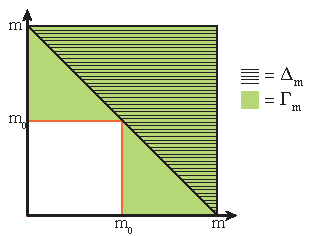
\includegraphics[scale=1.2]{Bilder/Menge_Gamma_Delta.pdf} \tag{Veranschaulichung}\]
Es folgt
\[
	E_m - E_{m_0} = \sum\limits_{(i,j) \in \Gamma_m} | a_i \cdot b_j |
\]
Es folgt
\begin{align*}
	|D_m -S_m | &= \left| \sum\limits_{(i,j) \in \Delta_m} a_i \cdot  b_j \right| \\
	&\le \sum\limits_{(i,j) \in \Delta_m} | a_i \cdot b_j | \\
	&\le \sum\limits_{(i,j) \in \Gamma_m} | a_i \cdot b_j | \\
	&< \varepsilon \quad \text{ falls } m >2m_0
\end{align*}
$\Rightarrow \lim\limits_{n \to \infty} (D_m -S_m) = 0$ \\
Absolute Konvergenz von $\sum\limits_{n=0}^{\infty} c_n$ : 
\vspace{10pt} \\
$\sum\limits_{n=0}^{\infty} |c_n|$ wird majorisiert durch $\sum\limits_{n=0}^{\infty} \overline{c_n}$, wo
\[
	\overline{c_n} := \sum\limits_{k=0}^{n} |a_{n-k} \cdot b_k|
\]
Aber $\sum\limits_{n=0}^{\infty} \overline{c_n}$ konvergiert, wie eben gesehen \hfill \( \square \)
% subsection cauchyprodukt_von_reihen (end)

\subsection{Beispiele} % (fold)
\label{sub:beispiele}
\begin{enumerate}[(i)]
	\item $\sum\limits_{n=0}^{\infty} \underbrace{\frac{n^2}{2^n}}_{=: a_n}$ konvergiert
	\vspace{10pt} \\
	Für $n \ge 3$ gilt
	\[
		\left| \frac{a_{n+1}}{a_n}\right| = \frac{(n+1)^2 2^n}{2^{n+1} n^2} = \frac{1}{2}\left( 1+ \frac{1}{n}\right) ^2
		\le \frac{1}{2} \left( 1+ \frac{1}{3}\right) ^2 = \underbrace{\frac{8}{9}}_{:= \theta} <1
	\]
	Quotientenkriterium $\Rightarrow$ Konvergenz
	\item Für $\sum\limits_{n=1}^{\infty} \frac{1}{n}$ gilt:
	\[
		\left| \frac{a_{n+1}}{a_n} \right| = \frac{n}{n+1} < 1
	\]
	aber $\sum\limits_{n=1}^{\infty} \frac{1}{n} $ divergiert
	\item Aber: $\sum\limits_{n=1}^{\infty} \frac{1}{n^2} $ konvergiert, obwohl
	\[
		\left| \frac{b_{n+1}}{b_n}\right| = \frac{n^2}{(n+1)^2} < 1 \text{ mit } \frac{n^2}{(n+1)^2} \xrightarrow{n \to \infty} 1
	\]
\end{enumerate}
% subsection beispiele (end)
% section reihen (end)

\section{Die Exponentialreihe} % (fold)
\label{sec:die_exponentialreihe}

\subsection{Definition und Satz} % (fold)
\label{sub:definition_und_satz}
Für jedes $x \in \mathds{R}$ konvergiert die Exponentialreihe 
\[
	\boxed{ \sum\limits_{n=0}^{\infty} \frac{x^n}{n!}}
\]
absolut. Den Limes bezeichnen wir mit $\exp (x)$. Wir setzen
\[
	e:= \exp(1) = \sum\limits_{n=0}^{\infty} \frac{1}{n!}
\]
Falls $N \in \mathds{N}$ und $|x| < \frac{N}{2} +1$ gilt 
\[
	\left| \sum\limits_{n=N+1}^{\infty}  \frac{x^n}{n!} \right| \le 2 \frac{|x|^{N+1}}{(N+1)!} 
\]
\underline{\textbf{Beweis:}} \\
\begin{itemize}
	\item Klar für $x=0$
	\item Für $x \not= 0$ und $ n\ge 2 |x|$
	\[
		\left| \frac{a_{n+1}}{a_n} \right| = \left| \frac{\frac{x^{n+1}}{(n+1)!}}{\frac{x^n}{n!}} \right| 
		= \frac{|x|}{n+1} \le \frac{1}{2}
	\]
	Quotientenkriterium $\Rightarrow$ absolute Konvergenz
	\item \textbf{\underline{Restgliedabschätzung}}
	\begin{align*}
		&\left| \sum\limits_{n=N+1}^{\infty} \frac{x^n}{n!}\right| \le \sum\limits_{n=N+1}^{\infty} \frac{|x|^n}{n!} \\
		= \enspace& \frac{|x|^{N+1}}{(N+1)!} \left( 1+ \frac{|x|}{N+2} + \frac{|x|^2}{(N+2)(N+3)} 
		+ \frac{|x|^3}{(N+2)(N+3)(N+4)} + \ldots  \right) \\
		\le \enspace & \frac{|x|^{N+1}}{(N+1)!} \left( 1+ \frac{|x|}{N+2} + \frac{|x|^2}{(N+2)^2} 
		+ \frac{|x|^3}{(N+2)^3} + \ldots \right)\\
		= \enspace &  \frac{|x|^{N+1}}{(N+1)!} \sum\limits_{k=0}^{\infty} \left(\frac{|x|}{N+2}\right)^k \\
		\le \enspace & \frac{|x|^{N+1}}{(N+1)!} \sum\limits_{k=0}^{\infty} \left(\frac{1}{2}\right)^k \tag{geometrische Reihe}\\
		= \enspace &  \frac{|x|^{N+1}}{(N+1)!} \cdot \frac{1}{1- \frac{1}{2}} = 2 \cdot \frac{|x|^{N+1}}{(N+1)!}
	\end{align*}
	\hfill \( \square \)
\end{itemize}
% subsection definition_und_satz (end)

\subsection{Satz: Funktionalgleichung von $\exp (.)$} % (fold)
\label{sub:funktionalgleichung_von_exp_}
Für $x,y \in \mathds{R}$ gilt 
\[
	\exp(x+y)= \exp (x) \cdot \exp (y)
\]
\underline{\textbf{Beweis:}} \\
$\exp (x)= \sum\limits_{n=0}^{\infty} \frac{x^n}{n!}$ und $\exp (y)= \sum\limits_{n=0}^{\infty}  \frac{y^n}{n!}$ konvergieren
absolut. Es gilt
\[
	c_n := \sum\limits_{k=0}^{n} \frac{x^{n-k}}{(n-k)!} \cdot \frac{y^k}{k!} = \frac{1}{n!} \sum\limits_{k=0}^{n}
	\frac{n!}{\underbrace{(n-k)! \cdot k!}_{\binom{n}{k}}} x^{n-k} \cdot y^k \overset{1.10}{=} \frac{1}{n!} \cdot (x+y)^n
\]
Also
\[
	\exp (x+y) = \sum\limits_{n=0}^{\infty} \frac{(x+y)^n}{n!} = \sum\limits_{n=0}^{\infty} c_n \overset{7.15}{=}
	\left(\sum\limits_{n=0}^{\infty} \frac{x^n}{n!}\right) \cdot  \left( \sum\limits_{n=0}^{\infty} \frac{y^n}{n!}\right)
	= \exp (x) \cdot  \exp (y)
\]
% subsection funktionalgleichung_von_exp_ (end)

\subsection{Corollar} % (fold)
\label{sub:corollar}
Für $x \in \mathds{R}$ gilt $\exp (-x)= \exp (x)^{-1}$ und $\exp (x)>0$. \\
Für $k \in \mathds{Z}$ gilt $\exp (k) = e^k$
\vspace{\baselineskip} \\
\underline{\textbf{Beweis:}} \\
\begin{itemize}
	\item 
	\[
	\exp (x) \cdot \exp (-x) \overset{8.2}{=} \exp (x-x) = \exp (0) = 1
	\]
	$\Rightarrow \exp (-x) = \exp (x)^{-1}$ \\
	Für $x \ge 0$ gilt $\exp (x)= \sum\limits_{n=0}^{\infty} \frac{x^n}{n!} \ge 1 >0$ \\
	Für $x < 0$ gilt $\exp (-x) >0$, also auch $\exp (x)= \exp (-x)^{-1} >0$
	\item Für $k=0$ gilt $\exp (0)= 1 = e^0.$ \\
	\underline{Induktion:} Für $k \in \mathds{N}$ gilt
	\begin{align*}
		\exp (k+1) &= \exp (k) \cdot \exp (1) \tag{folgt aus 8.2} \\
		&= \exp (k) \cdot e \\
		&= e^k \cdot e = e^{k+1}
	\end{align*}
	$\Rightarrow \exp (k) = e^k \enspace \forall k \in \mathds{N}$ \\
	$\exp (-k)= (\exp (k))^{-1} = (e^k)^{-1} = e^{-k} \quad \forall k \in \mathds{N}$
\end{itemize}
% subsection corollar (end)
% section die_exponentialreihe (end)

\section{Stetige Funktionen} % (fold)
\label{sec:stetige_funktionen}

\subsection{Definition} % (fold)
\label{sub:definition}
Sei $D \subset \mathds{R}$. Sei $f: D \to \mathds{R}$ eine Funktion. $f$ heißt stetig in $x_0 \in D$, falls gilt
\[
	\forall \varepsilon >0 \enspace \exists \delta >0 : \forall x \in D : \big( |x-x_0| < \delta \Rightarrow |f(x)-f(x_0)|< \varepsilon \big)
\]
$f$ heißt \underline{\textbf{stetig}}, falls $f$ stetig ist in $x_0$ ist für jedes $x_0 \in D$. 
\[
	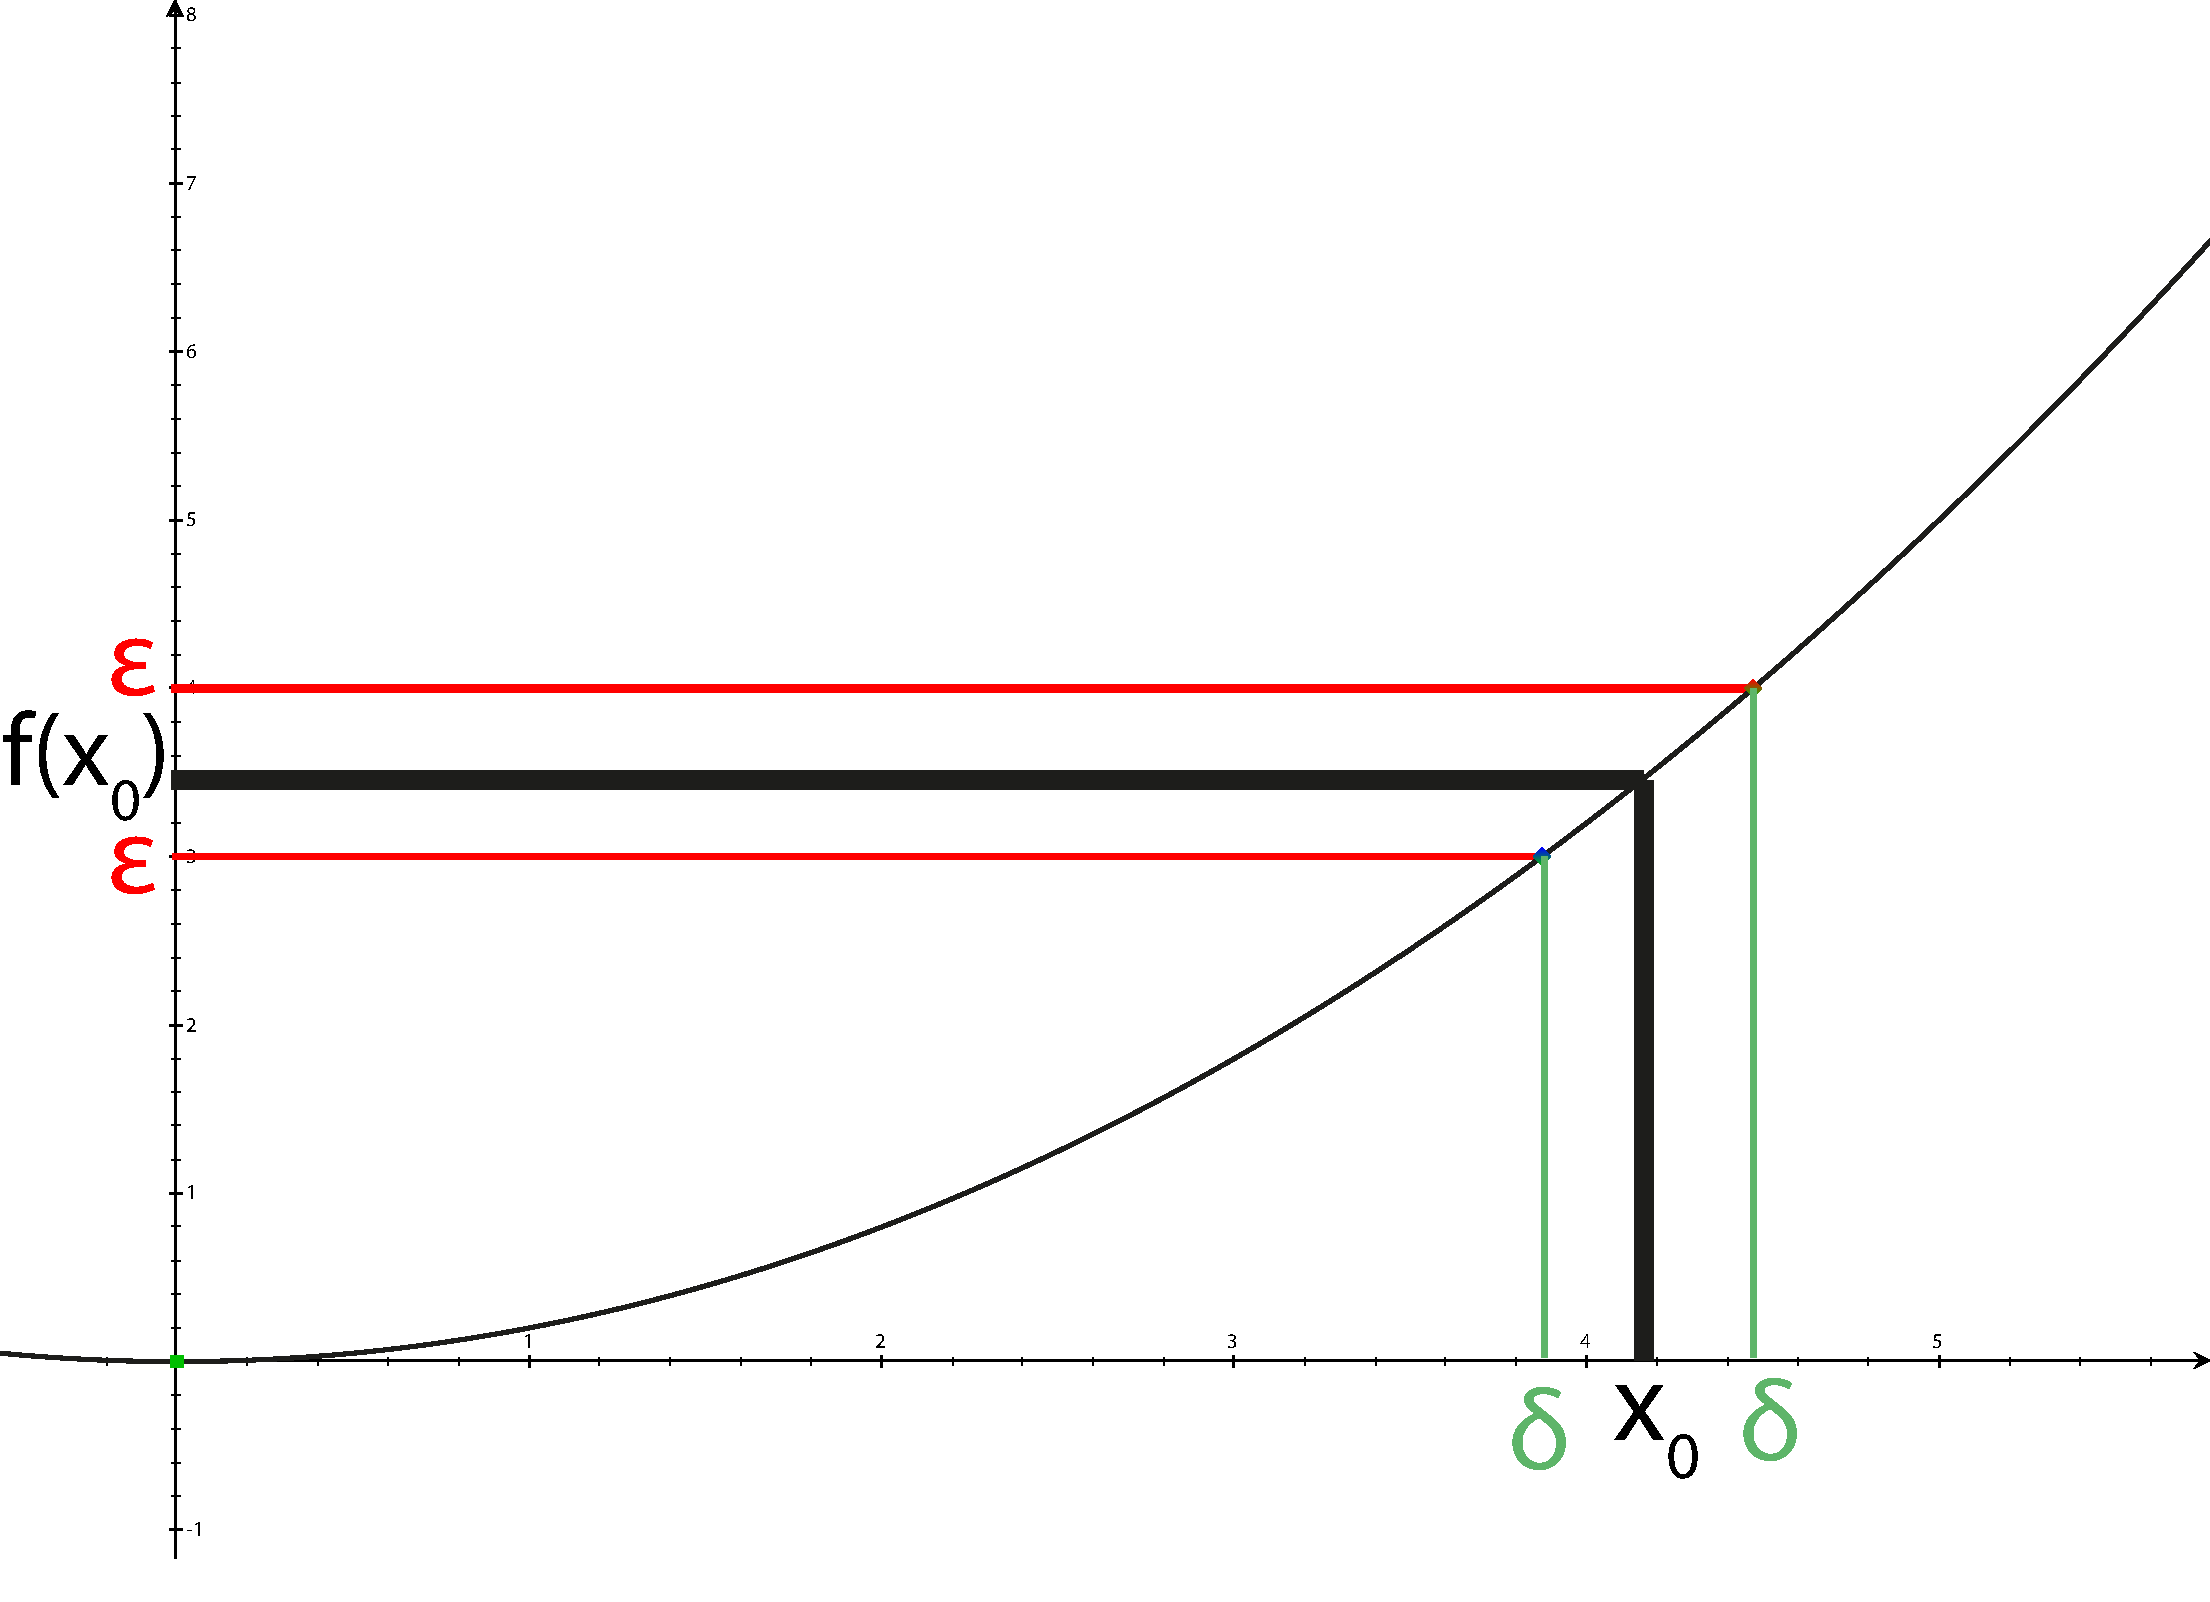
\includegraphics[scale=0.18]{Bilder/Stetigkeit.pdf}
\] 
% subsection definition (end)

\subsection{Beispiele} % (fold)
\label{sub:beispiel}
\begin{enumerate}[(i)]
	\item $\id : \mathds{R} \to \mathds{R}$ ist stetig. 
	\vspace{10pt} \\
	Sei $x_0 \in \mathds{R}$. Sei $\varepsilon >0$. Setze $\delta := \varepsilon$.
	Falls $|x-x_0|< \delta$, so gilt
	\[
		\big|\id (x) -\id (x_0) \big| = |x - x_0| < \delta = \varepsilon
	\]
	\item  $f : \mathds{R} \to \mathds{R} \quad x \mapsto x^2$ ist stetig.
	\vspace{10pt} \\
	Sei $x_0 \in \mathds{R}$. Sei $\varepsilon >0$. Setze $\delta 
	:= \min \{ 1, \frac{\varepsilon}{2 |x_0| +1} \}$. \\
	Sei nun $x \in \mathds{R}$ mit $|x - x_0|< \delta$. Dann
	\begin{align*}
		|f(x)-f(x_0)|= |x^2 - x_0^2| &= |x-x_0| \cdot |x +x_0 |
		\tag{Hinzufügen: $-x_0 +x_0$}\\
		&\le |x -x _0| \cdot \big(|x-x_0| +2 |x_0|\big) \\
		&\lneq \frac{\varepsilon}{2 |x_0| +1} \big( 1+ 2|x_0|\big) \\
		&= \varepsilon
	\end{align*}
	\item $f : \mathds{R}_+ \to \mathds{R} \quad x \mapsto \sqrt{x}$ ist stetig
	\vspace{10pt} \\
	Sei $x_0 \in \mathds{R}_+$. Sei $\varepsilon >0$. Setze $ \delta := \frac{\varepsilon^2}{2} $. Sei nun $x \in \mathds{R}_+$ mit $|x-x_0|<\delta$. \\
	Falls $x\ge x_0$ gilt, dann 
	\begin{align*}
		|f(x)-f(x_0)|^2 &= |\sqrt{x} - \sqrt{x_0}|^2 \tag{2. binomische Formel}\\
		&= \left| x - \sqrt{xx_0} - \sqrt{xx_0}+x_0 \right| \tag{Dreiecksungleichug}\\
		&\le |x-\sqrt{xx_0}| + |\sqrt{xx_0} - x_0| \tag{da $x\ge x_0$} \\
		&= x- \sqrt{x} \sqrt{x_0} + \sqrt{x} \sqrt{x_0} -x_0  \\
		&\le x -\sqrt{x_0} \sqrt{x_0} + \sqrt{x} \sqrt{x} -x_0 \\
		&= x -x_0 + x - x_0 \\
		&\le 2 \cdot |x-x_0| \\
		&\le 2 \cdot \delta \\
		&= 2 \cdot \frac{\varepsilon^2}{2} = \varepsilon^2 
	\end{align*}
	$\Rightarrow |f(x)-f(x_0)|< \varepsilon$ Ebenso für $x<x_0$ \hfill \(\square\) 
	\item 
	$f : \mathds{Q} \to \mathds{R}\quad f(x):= 
	\begin{cases}
		1, &\text{ falls }x > \sqrt{2} \\
		-1 , &\text{ falls }x < \sqrt{2} 
	\end{cases} \enspace$ ist stetig.
	\vspace{7pt} \\
	Beweis: Übung!
	\item $f : \mathds{R} \to \mathds{R} \quad f(x):= 
	\begin{cases}
		1, &\text{ falls }x \in \mathds{Q}\\
		0, &\text{ falls }x \not\in \mathds{Q}
		\end{cases} \enspace$ ist in keinem Punkt stetig.
		\item $\exp : \mathds{R} \to \mathds{R}$ ist stetig.
	\vspace{7pt} \\
	Übung!	
\end{enumerate}
% subsection beispiel (end)

\subsection{Defintion} % (fold)
\label{sub:defintion}
$f : D \to \mathds{R}$ heißt \underline{\textbf{Lipschitz stetig}}, falls $L \in \mathds{R}_+$ existiert mit:
\[
	\forall x,y \in D : \big| f(x)-f(y) \big| \le L \cdot |x-y|
\]
% subsection defintion (end)

\subsection{Beispiele} % (fold)
\label{sub:beispiele}
\begin{enumerate}[(i)]
	\item $x \mapsto ax+b$ ist Lipschitz mit $L=|a|$
	\item $x \mapsto |x|$ ist Lipschitz mit $L=1$
	\item $f: [a, \infty) \to \mathds{R} \quad x \mapsto \sqrt{x} $
	ist Lipschitz für $a>0$. Ist nicht Lipschitz für $a=0$
	\item $g: \mathds{R} \to \mathds{R} \quad x \mapsto x^2$ ist nicht Lipschitz. \\
	\underline{Aber}: $g|_{[a,b]}$ ist Lipschitz
	\[
		g|_{[a,b]} : [a,b] \to \mathds{R} \quad x \mapsto x^2 \tag{Übung!}
	\]
	\item Lipschitz stetig $\Rightarrow $ stetig $\left(\delta = \frac{\varepsilon}{L} \right)$
\end{enumerate}
% subsection beispiele (end)

\subsection{Proposition} % (fold)
\label{sub:proposition}
Sei $f: D \to \mathds{R} \enspace , \enspace \bar x \in D$. \\
Dann sind folgende Aussagen äquivalent:
\begin{enumerate}[(i)]
	\item $f$ ist stetig in $\bar x$
	\item für jede Folge $(x_n)_{n \in \mathds{N}} \subset D$ mit 
	$\lim\limits_{n \to \infty} x_n = \bar x$ gilt:
	\[
		\lim\limits_{n \to \infty} f(x_n) = f(\bar x)
	\]
\end{enumerate}
\underline{\textbf{Beweis:}} (i)$\Rightarrow$(ii)\\
Sei $(x_n)_{n \in \mathds{N}} \subset D$ eine Folge mit $\lim\limits_{n \to \infty} x_n = \bar x$. Sei $\varepsilon>0$.
\vspace{10pt} \\
$f$ ist stetig in $\bar x \Longrightarrow \exists \delta >0$ mit 
\[
	|x- \bar x|< \delta \Longrightarrow |f(x)-f(\bar x)|< \varepsilon \tag{$\star$}
\] 
$x_n \xrightarrow{n \to \infty} \bar x \Rightarrow \exists N \in \mathds{N}$ mit
$|x_n - \bar x|< \delta \enspace \forall n \geq N$. Dann gilt für $n \geq N$
\[
	|x_n - \bar x| < \delta \overset{(\star)}{\Rightarrow} |f(x_n)- f(\bar x)|<
	\varepsilon \Rightarrow f(x_n) \xrightarrow{n \to \infty} f(\bar x)
\]
\underline{(ii) $\Rightarrow$ (i)} \\
Angenommen: $f$ ist nicht stetig in $\bar x$. Das heißt
\[
	\exists \varepsilon >0 : \forall \delta>0 : \exists x \in D : |x - \bar x|< \delta
	\enspace \text{ und } \enspace |f(x)-f(\bar x)| \ge \varepsilon
\]
Es folgt 
\[
	\forall n \in \mathds{N} \enspace \exists x_n \in D : |x_n - \bar x|< 
	\frac{1}{n+1} \enspace \text{ und } \enspace |f(x_n)- f(\bar x)| \geq \varepsilon
\]
Dann gilt: 
\[
	x_n \xrightarrow{n \to \infty} \bar x \enspace , \text{aber } \enspace
	f(x_n) \not\xrightarrow{n \to \infty} f(\bar x)
\] Wir haben gezeigt:
$\neg \text{(i)} \Rightarrow  \neg \text{(ii), also (ii)} \Rightarrow \text{(i)}$ \hfill \( \square \)
% subsection proposition (end)

\subsection{Proposition} % (fold)
\label{sub:proposition}
Seien $f,g,h : D \to \mathds{R}$ stetig in $\bar x \in D$. Dann sind $f+g$ und $f \cdot g$ stetig in $\bar x$. Falls 
$h(x)\not= 0$ für alle $x \in D$, so ist $\frac{f}{h}$ stetig in $\bar x$.
\vspace{\baselineskip} \\
\underline{\textbf{Beweis}:} \\
Sei $(x_n)_{n \in \mathds{N}} \subset D$ mit $x_n \xrightarrow{n \to \infty} \bar x$. Dann gilt
\[
	\begin{array}{ccc}
	(f+g)(x_n) = f(x_n) +g(x_n) & \xrightarrow{n \to \infty} & f(\bar x) + g(\bar x) = (f+g)(\bar x) \\
	& \downarrow & \\
	& f,g \text{ stetig} & \\
	& \text{9.5 (i) $\Rightarrow$ (ii)} & \\
	& \text{Prop 5.7} &
	\end{array}
\]
$\overset{\text{9.5 (ii)$\Rightarrow$(i) }}\Longrightarrow $ $f+g$ stetig in $\bar x$. Ebenso $f \cdot g$ und $\frac{f}{h}$
\hfill \( \square \)
% subsection proposition (end)

\subsection{Proposition} % (fold)
\label{sub:proposition}
Seien $f: D \to \mathds{R}$, $g: E \to \mathds{R}$ Funktionen mit $E \supset f(D)$. Falls $f$ stetig in $\bar x \in D$ und $g$
stetig ist in $f(\bar x) \in E$, dann gilt $g \circ f$ ist stetig in $\bar x$
\vspace{\baselineskip} \\
\underline{\textbf{Beweis:}} \\
Sei $(x_n)_{n \in \mathds{N}} \in D$ eine Folge mit $x_n \xrightarrow{n \to \infty} \bar x$.
\[
	f \text{ stetig in } \bar x \Rightarrow f(x_n) \xrightarrow{n \to \infty} f(\bar x)
\]
Wir haben jetzt:
\[
	\big(f(x_n)\big)_{n \in \mathds{N}} \subset E \qquad f(x_n) \xrightarrow{n \to \infty} f(\bar x)
\]
Es folgt:
\[
	g \text{ stetig in} f(\bar x) \Rightarrow \underset{\underset{(g \circ f)(x_n)}{\parallel}}{g\big(f(x_n)\big)} 
	\xrightarrow{n \to \infty} g\big(f(\bar x)\big) = (g \circ f)(\bar x)
\] \hfill \( \square \)
% subsection proposition (end)

\subsection{Beispiel} % (fold)
\label{sub:beispiel}
Eine Polynom $p$ ist eine Funktion der Form
\[
	x \mapsto p(x) = \alpha_0 + \alpha_1 x + \alpha_2 x^2\ldots + \alpha_n x^n
\]
wo $\alpha_i \in \mathds{R}$ (Dann $p: \mathds{R} \to \mathds{R}$)
\begin{enumerate}[(i)]
	\item Polynome sind stetig auf $\mathds{R}$
	\item Seien $p,q$ Polynome $D:= \{ x \in \mathds{R} \mid q(x) \not= 0\}$ \\
	Dann ist $\frac{p}{q}$ stetig auf $D$ ($\frac{p}{q}$ heißt rationale Funktion)
\end{enumerate}
% subsection beispiel (end)

\subsection{Bemerkung} % (fold)
\label{sub:bemerkung}
"'$\varepsilon$-$\delta$-Definition"' von Stetigkeit lässt sich geometrisch interpretieren.
% subsection bemerkung (end)

\subsection{Satz: Zwischenwertsatz} % (fold)
\label{sub:satz_zwischenwertsatz}
Sei $a\le b$ und $f: [a,b] \to \mathds{R}$ stetig. \\
Zu jedem $\gamma$ zwischen $f(a)$ und $f(b)$ existiert ein $c \in [a,b]$ mit $f(c)=\gamma$
\vspace{\baselineskip} \\
\underline{\textbf{Beweis:}} \\
O.E.d.A sei $f(a) \le \gamma \le f(b)$. Setze $[a_0 , b_0]:= [a,b]$ dann gilt $\gamma \in \big[f(a_0), f(b_0)\big]$. \\
Seien $[a_n , b_n]$ bereits konstruiert mit 
\begin{enumerate}[(i)]
	\item $\gamma \in \big[ f(a_n), f(b_n)\big]$
	\item $[a_n b_n] \subset [a_{n-1}, b_{n-1}]$ und $b_n -a_n = 2^{-n} (b-a)$
\end{enumerate}
Dann gilt 
\[
	\gamma \in \big[ f(a_n), f(b_n) \big] \subset \left[ f(a_n) , f\left(\frac{a_n +b_n}{2} \right) \right] \cup
	\left[f\left(\frac{a_n +b_n}{2}\right), f(b_n) \right]
\]
Setze
\[
	[a_{n+1}, b_{n+1}] := 
	\begin{cases}
		\left[a_n , \frac{a_n + b_n}{2} \right], &\text{ falls }\gamma \in 
		\left[ f(a_n), f \left( \frac{a_n +b_n}{2} \right) \right]\\
		\left[\frac{a_n + b_n}{2} , b_n\right] , &\text{ sonst}
	\end{cases}
\]
Induktion $\leadsto$ Intervallschachtelung $[a_n , b_n] n \in \mathds{N} $ mit
\[
	\exists c \in \bigcap_{n \in \mathds{N}} [a_n , b_n]
\]
Außerdem $a_n \xrightarrow{n \to \infty} c$ und $b_n  \xrightarrow{n \to \infty} c$
\[
	f  \text{ ist stetig } \Longrightarrow f(a_n) \xrightarrow{n \to \infty} f(c) \enspace \wedge \enspace f(b_n) \xrightarrow{n \to \infty} f(c) 
\]
$f(a_n) \le \gamma \le f(b_n)$ für $n \in \mathds{N}$
\[
	\Rightarrow f(c) = \lim\limits_{n \to \infty} f(a_n) \le \gamma \le \lim\limits_{n \to \infty} f(b_n) = f(c)
\]
$\Rightarrow \gamma = f(c)$ \hfill \( \square \)
% subsection satz_zwischenwertsatz (end)

\subsection{Beispiel} % (fold)
\label{sub:beispiel}
Jedes Polynom ungeraden Grades besitzt eine Nullstelle.
% subsection beispiel (end)

\subsection{Satz} % (fold)
\label{sub:satz}
Sei $a \le b$. Jede stetige Funktion $f : [a,b] \to \mathds{R}$ nimmt ihr Maximum und ihr Minimum an. \\
D.h. es gibt $s,t \in [a,b]$ mit
\[
	\begin{array}{cll}
	f(s) &= \sup & \{ f(x) \mid x \in [a,b] \} \\
	f(t) &= \inf & \{ f(x) \mid x \in [a,b] \}
	\end{array}
\] 
\underline{\textbf{Beweis:}} \\
Setze 
\[
	M:= \sup \big\{ f(x) \mid x \in [a,b]\big\} \in \mathds{R} \cup \{ \infty\}
\]
{\small ($M= \infty$ falls $\{f(x) \mid x \in [a,b] \}$ nicht nach oben beschränkt ist)}
\vspace{10pt} \\
Dann existiert eine Folge $(y_n)_{n \in \mathds{N}} \subset \{ f(x) \mid x \in [a,b] \}$ mit $y_n \xrightarrow{n \to \infty} M$
(warum?) \\
$\Rightarrow $ es existiert eine Folge $(x_n)_{n \in \mathds{N}} \subset [a,b]$ mit $f(x_n) = y_n \xrightarrow{n \to \infty} M$ 
\vspace{10pt} \\
Nach Bolzano-Weierstraß $\Rightarrow$ $x_n$ besitzt konvergente Teilfolge $(x_{n_k})_{k \in \mathds{N}}$.  \\
Sei $s:= \lim\limits_{k \to \infty} x_{n_k}$ Es gilt $a \le x_{n_k} \le b$ für alle $k \in \mathds{N}$. Also muss gelten:
\[
	\begin{array}{rl}
	\Rightarrow & a \le \underset{\underset{s}{\shortparallel}}{\lim\limits_{k \to \infty} x_{n_k}} \le b \tag{nach 5.9} \\
	\Rightarrow & s \in [a,b] \\
	f \text{ stetig } \Rightarrow & M= \lim\limits_{n \to \infty} f(x_n) =\lim\limits_{k \to \infty} f(x_{n_k}) 
	= f(\lim\limits_{k \to \infty} x_{n_k}) = f(s)
\end{array}
\]
$f \leadsto -f$ ergibt Aussage für das Minimum \hfill \( \square \)
% subsection satz (end)

\subsection{Definition} % (fold)
\label{sub:definition}
$f : D \to \mathds{R}$ ist gleichmäßig stetig, falls gilt
\[
	\forall \varepsilon > 0 \enspace \exists \delta >0 : \forall x,x' \in D : \big( |x-x'|< \delta \Rightarrow |f(x)-f(x')| < \varepsilon \big)
\]
% subsection definitionen (end)

\subsection{Bemerkung} % (fold)
\label{sub:bemerkung}
\[
	\text{gleichmäßig stetig } \underset{\not\Leftarrow}{\Longrightarrow} \text{ stetig}
\]
\underline{\textbf{Beweis:}} \\
"'($\Rightarrow $)"' ist trivial
\vspace{10pt} \\
"'$\not\Leftarrow$"' :\\
$f: (0, \infty) \to \mathds{R} \quad x \mapsto \frac{1}{x} $ ist stetig. Sei $\varepsilon = 1$. Sei $\delta >0$. Wähle
$n \in \mathds{N}^* $ mit $| \frac{1}{n} - \frac{1}{2n}| < \delta $. Dann
\[
	\left| f\left(\frac{1}{n}\right) - f\left( \frac{1}{2n}\right) \right| = |n-2n| = n \ge \varepsilon
\]
\hfill \( \square \)
% subsection bemerkung (end)

\subsection{Satz} % (fold)
\label{sub:satz}
Sei $f: [a,b] \to \mathds{R}$ stetig
\[
	\Rightarrow f \text{ ist gleichmäßig stetig}
\]
\underline{\textbf{Beweis:}} \\
Annahme: $f$ ist nicht gleichmäßig stetig. dann
\[
	\exists \varepsilon > 0 \enspace \forall \delta >0 : \exists x,x' \in D : |x-x'| < \delta \enspace \wedge \enspace |f(x)- f(-x)| \ge \varepsilon
\]
Zu $\delta = \frac{1}{n+1}$ existieren $x_n , x'_n \in [a,b]$ mit $|x_n - x'_n|< \frac{1}{n+1} $ und $ \big| f(x_n)-f(x'_n)\big| \ge \varepsilon$
\[
	\leadsto \text{ Folgen } (x_n)_{n \in \mathds{N}} , (x_n)_{n \in \mathds{N}} \subset [a,b]
\]
Bolzano-Weierstraß $\leadsto$ konvergente Teilfolgen $\left( x_{n_k} \right) _{k \in \mathds{N}}$ und $ \left( x'_{n_k} \right) _{k \in \mathds{N}}$.
Dann gilt
\[
	\overline{x} := \lim\limits_{k \to \infty} x_{n_k} = \lim\limits_{k \to \infty} x'_{n_k} \in [a,b]
\] 
$f$ stetig $\Rightarrow $
\[
	\lim\limits_{k \to \infty} f \left(x_{n_k}\right) = f \left( \lim\limits_{k \to \infty} x_{n_k}\right) = f( \overline{x}) = 
	f \left( \lim\limits_{k \to \infty} x'_{n_k}\right)  = \lim\limits_{k \to \infty} f \left(x'_{n_k}\right)
\]
$\Rightarrow \left| f\left(x_{n_k}\right) - f \left(x'_{n_k}\right) \right| \xrightarrow{k \to \infty} 0$ \quad {\huge $\lightning$} 
zu $ \left| f(x_n) - f(x'_n)\right| \ge \varepsilon$ \hfill \( \square \) 
\vspace{10pt} \\
\hrule 
\vspace{10pt} 
\textbf{Korrektur:} Wähle zuert Teilfolge $ \left(x_{n_k}\right)_{k \in \mathds{N}}$ mit $ \left(x_{n_k}\right) \xrightarrow{k \to \infty} \overline{x}$.
$ \left(x'_{n_k}\right)_{k \in \mathds{N}} \subset [a,b]$ besitzt konvergente Teilfolge $ \left(x'_{n_{k_l}}\right)_{l \in \mathds{N}}$, die auch gegen 
$\overline{x}$ konvergiert.

% subsection satz (end)

\subsection{Definition} % (fold)
\label{sub:definition}
$f: D \to \mathds{R}$ heißt (streng) monoton wachsend, falls gilt
\[
	x,x' \in D , x < x' \Rightarrow f(x) \le f(x') \qquad \big(\Rightarrow f(x) < f(x')\big)
\]
$f: D \to \mathds{R}$ heißt (streng) monoton fallend, falls gilt
\[
	x,x' \in D , x < x' \Rightarrow f(x) \ge f(x') \qquad \big(\Rightarrow f(x) > f(x')\big)
\]
% subsection definition (end)

\subsection{Satz} % (fold)
\label{sub:satz}
Sei $a \le b , f: [a,b] \to \mathds{R}$ stetig und streng monoton wachsend (oder auch streng monoton fallend).
\vspace{10pt} \\
Dann ist $f: [a,b] \to \left[f(a), f(b)\right]$ (bzw. $f: [a,b] \to \left[f(b), f(a)\right]$) bijektiv und die Umkehrabbildung $f ^{-1}$ ist ebenfalls stetig und streng monoton wachsend bzw. streng monoton fallend.
\vspace{\baselineskip} \\
\underline{\textbf{Beweis:}} \\
Sei $f$ O.E.d.A streng monoton wachsend. \\
$f$ injektiv: trivial (aufgrund der strengen Monotonie)
\vspace{10pt} \\
$f$ surjektiv: \\
\begin{gather*}
	a < x b \Rightarrow f(a) < f(x) < f(b) \\
	\Rightarrow f \left([a,b]\right) \subset \left[ f(a), f(b)\right] \\
	\text{nach dem Zwischenwertsatz gilt } \enspace f \left( [a,b]\right) = \left[f(a), f(b)\right]
\end{gather*}
$\Rightarrow $ $f$ ist bijektiv
\vspace{\baselineskip} \\
Sei nun $f ^{-1} : [f(a), f(b)] \to [a,b]$ die Umkehrfunktion von $f$. 
\vspace{10pt} \\
$f ^{-1}$ ist streng monoton wachsend: klar (warum?)
\vspace{10pt} \\
\underline{Beweis der Stetigkeit von $f ^{-1}$ (Widerspruchsbeweis)} \\
Angenommen $f ^{-1}$ ist nicht stetig. Dann existiert $\overline{y} \in [f(a), f(b)]$ und eine Folge 
$(y_n)_{n \in \mathds{N} } \subset [f(a), f(b)]$ mit $\lim\limits_{n \to \infty} y_n = \overline{y}$, aber 
$f ^{-1} (y_n) \not\xrightarrow{n \to \infty} f ^{-1} (\overline{y})$
\[
	\Rightarrow \exists \varepsilon >0 \text{ und Teilfolge } (y_{n_k})_{k \in \mathds{N}} \text{ mit } 
	\left| f ^{-1} (y_{n_k}) - f ^{-1} (\overline{y})\right| \ge \varepsilon \enspace \forall k \in \mathds{N}
\]
(Negation 9.5 (ii))
\vspace{\baselineskip} \\
Nach Bolzano-Weierstraß existiert eine Teilfolge der Teilfolge $ f^{-1} \left( \left(y_{n_k}\right)_{k \in \mathds{N}}\right) $
\[
	f ^{-1} \left(y_{n_{k_l}}\right)_{l \in \mathds{N}} 
\]
mit
\[
	\lim\limits_{l \to \infty} f ^{-1} \left(y_{n_{k_l}}\right) = \overline{x} \enspace \text{ für ein } \enspace \overline{x} \in [a,b]
\]
Dann gilt: $\left| f ^{-1} \left(y_{n_{k_l}}\right) - f ^{-1} (\overline{y}) \right| \ge \varepsilon$ also auch 
$\left| \overline{x} - f ^{-1}(\overline{y}) \right| \ge \varepsilon$. Andererseits gilt:
\[
	\overline{y}= \lim\limits_{l \to \infty} y_{n_{k_l}} = \lim\limits_{l \to \infty} f \circ f ^{-1} \left(y_{n_{k_l}}\right) 
	\overset{f \text{ stetig}}{=} f \left( \lim\limits_{l \to \infty} f ^{-1} \left(y_{n_{k_l}}\right) \right) = f (\overline{x})	
\]
also auch
\[
	f ^{-1} (\overline{y}) = f ^{-1} \left( f (\overline{x})\right) = \overline{x} \quad \text{ {\huge $\lightning$}}
\]
\hfill \( \square \)
% subsection satz (end)

\subsection{Bemerkung} % (fold)
\label{sub:bemerkung}
Allgemeiner gilt: Sei $I \subset \mathds{R}$ ein Intervall, $f: I \to \mathds{R}$ stetig und streng monoton wachsend (streng monoton fallend). Dann ist 
$f(I)$ ein Intervall und $f : I \to f(I)$ ist bijektiv. $f ^{-1} : f(I) \to I$ ist wieder streng monoton wachsend (streng monoton fallend) und stetig.
\vspace{\baselineskip} \\
\underline{\textbf{Beweis:}} \\
Übung Blatt 4 Aufgabe 1
% subsection bemerkung (end)

\subsection{Beispiel} % (fold)
\label{sub:beispiel}
Sei $k \in \mathds{N}^*$, dann ist $f : \mathds{R}_+ \to \mathds{R}_+ \quad x \mapsto x^k$ streng monoton wachsend (Bemerkung 2.5(vi) + Induktion)
\[
	\Rightarrow \exists \text{ stetige und streng monoton wachsende Umkehrfunktion } \enspace f ^{-1} : \mathds{R}_+ \to \mathds{R}_+
\]
Wegen Eindeutigkeit der $k$-ten Wurzel gilt
\[
	f ^{-1} (y) = \sqrt[k]{y} \qquad \text{ (vergleiche Satz 3.3)}
\]
% subsection beispiel (end)

\subsection{Definition und Satz} % (fold)
\label{sub:definition_und_satz}
$\exp : \mathds{R} \to (0, \infty)$ besitzt eine stetige und streng monoton wachsende Umkehrfunktion $\ln : (0, \infty) \to \mathds{R}$. Es gilt 
\[
	\ln (x \cdot y) = \ln (x) + \ln (y) \qquad \text{ für } x,y \in (0, \infty)
\]
\underline{\textbf{Beweis:}} \\
$\exp$ ist stetig und streng monoton wachsend nach Übung. \\
$\exp : \mathds{R} \to (0, \infty)$ ist surjektiv nach Zwischenwertsatz (warum?)
\vspace{10pt} \\
9.17/9.18 $\Rightarrow $ Umkehrfunktion $\ln : (0, \infty) \to \mathds{R}$ stetig und streng monoton wachsend
\begin{align*}
	\ln (x \cdot y) &= \ln \Big( \exp \big(\ln (x) \big)  \cdot \exp \big(\ln (y) \big) \Big) \\
	&= \ln \big(\exp (\ln x + \ln y) \big) \\
	&= \ln x + \ln y
\end{align*}
\hfill \( \square \)
% subsection definition_und_satz (end)

\subsection{Definition und Proposition} % (fold)
\label{sub:definition_und_proposition}
Für $a >0$ setzen wir
\[
	a^x := \exp (x \cdot  \ln a) \quad x \in \mathds{R}
\]
Es gilt $a^{x+y}= a^x \cdot a^y , x,y \in \mathds{R}$. Für $x=\frac{p}{q} \in \mathds{Q}$ stimmt die Definition mit der früheren überein, das heißt
\[
	\exp \left(\frac{p}{q} \cdot \ln a \right) = \sqrt[q]{a^p}
\]
\underline{\textbf{Beweis:}} \\
\begin{enumerate}[(i)]
	\item 
	\begin{align*}
		a^{x+y} &= \exp ((x+y) \ln a) \\
		&= \exp (x \ln a + y \ln a) \\
		&= \exp (x \ln a) \cdot \exp (y \ln a) \\
		&= a^x \cdot a^y
	\end{align*}
	\item 
	\begin{align*}
		\left(\exp \left(\frac{p}{q} \ln a \right)\right)^q &= \exp \underbrace{\left(\frac{p}{q} \ln a + 
				\frac{p}{q} \ln a + \ldots + \frac{p}{q} \ln a \right)}_{\text{$q$-mal}} \\
		&= \exp (p \cdot \ln a) \\
		&= a^p \\
		\exp \left(\frac{p}{q} \ln a \right) &= \sqrt[q]{a^p}
	\end{align*}
	wegen Eindeutigkeit der $q$-ten Wurzel \hfill \( \square \)
\end{enumerate}
% subsection definition_und_proposition (end)

\subsection{Bemerkung} % (fold)
\label{sub:bemerkung}
\begin{enumerate}[(i)]
	\item Für $a>0$ gilt $\lim\limits_{n \to \infty} \sqrt[n]{a}=1$
	\item \begin{align*}
		(a^x)^y &= a^{xy} \\
		a^x b^x &= (ab)^x \\
		(a^{-1})^x &= a^{-x} \\
		\ln a^x &= x \cdot \ln a \qquad a,b>0 \enspace x,y \in \mathds{R}
	\end{align*}
\end{enumerate}
\underline{\textbf{Beweis:}} \\
\begin{enumerate}[(i)]
	\item
	\[
		a^{\frac{1}{n} }  =\exp \left( \frac{1}{n} \cdot \ln a \right) \underset{\exp \text{ stetig}}{\xrightarrow{n \to \infty}} \exp (0) = 1
	\]
	\item Übung
\end{enumerate}
% subsection bemerkung (end)

\subsection{Satz} % (fold)
\label{sub:satz}
Sei $f: \mathds{R} \to \mathds{R}$ stetig mit $f(x+y)=f(x) \cdot f(y) \forall x,y \in \mathds{R}$. Dann gilt 
\[
	f \underbrace{\equiv}_{\text{genau äquivalent}} 0 \quad \left(f(x)=0 \enspace \forall x\right) 
\]
oder
\[
	f(x)=a^x \text{ mit } a=f(1)>0
\]
% subsection satz (end)

\subsection{Definition} % (fold)
\label{sub:definition}
Sei $f: D \to \mathds{R}$ eine Funktion, $a \in [- \infty , + \infty] = \mathds{R} \cup \{ - \infty\} \cup \{ + \infty \}$ ein Punkt, so dass
eine Folge $(a_n)_{n \in \mathds{N}} \subset D$ existiert mit $\lim\limits_{n \to \infty} a_n = a$ \\
Sei $b \in [- \infty , + \infty]$
\begin{enumerate}[(i)]
	\item Wir schreiben $\lim\limits_{x \to \infty} f(x) = b$ falls gilt:
	\[
		\text{Für jede Folge } (x_n)_{n \in \mathds{N} } \subset D \text{ mit } \lim\limits_{n \to \infty} x_n = a \text{ gilt } \lim\limits_{n \to \infty} f(x_n)=b
	\]
	\item Wir schreiben $\lim\limits_{x \searrow a} f(x) =b $, falls gilt
	\[
		\text{Für jede Folge } (x_n)_{n \in \mathds{N}} \subset D \cap (a, \infty) \text{ mit } \lim\limits_{n \to \infty} x_n =a \text{ gilt } 
		\lim\limits_{n \to \infty} f(x_n)=b
	\]
	(falls eine Folge $(a_n)_{n \in \mathds{N}} \subset D \cap (a; \infty)$ exisitert mit $\lim\limits_{n \to \infty} a_n = a$)
	\item Analog für $\lim\limits_{x \nearrow a} f(x) = b $
\end{enumerate}
% subsection definition (end)

\subsection{Beispiele} % (fold)
\label{sub:beispiele}
\begin{enumerate}[(i)]
	\item Für $k \in \mathds{N}$ gilt:
	\[
		\lim\limits_{x \to \infty} \frac{e^x}{x^k} = \infty \qquad \left( \frac{e^x}{x^k} : (0, \infty) \to \mathds{R} \right) 
	\]
	Für $x>0$ gilt
	\[
		e^x = \sum\limits_{n=0}^{\infty} \frac{x^n}{n!} > \frac{x^{k+1}}{(k+1)!} \quad \text{also} 
		\quad \frac{e^x}{x^k} > \frac{x}{(k+1)!}  \xrightarrow{x \to \infty} \infty
	\]
	Genauer: Sei $(x_n)_{n \in \mathds{N}} \subset (0, \infty)$ eine Folge mit $\lim\limits_{n \to \infty} x_n = \infty$. Zu zeigen:
	\[
		\lim\limits_{n \to \infty} \frac{e^{x_n}}{x_n^k} = \infty 
	\]
	Sei $K \in \mathds{R}$. Wähle $N \in \mathds{N}$ so, dass $x_n \ge K \cdot (k+1)!$ falls $n \ge N$. Dann gilt
	\[
		\frac{e^{x_n}}{x_n^k} > \frac{x_n}{(k+1)!} \ge K \quad \text{ falls } n \ge N  
	\]
	\hfill \( \square \)
	\item Für $k \in \mathds{N}$ gilt
	\[
		\lim\limits_{x \to \infty} x^k e^{-x} =0 \quad \xrightarrow{x \not= 0} \quad \lim\limits_{x \to \infty} \left( \frac{e^x}{x^k} \right)^{-1} =0 
		\tag{folgt aus Beispiel (i)}
	\]
	Es gilt
	\[
		\lim\limits_{x \searrow 0} x^k e^{\frac{1}{x} } = 0 
	\]
	da (Substitution $y_n := \frac{1}{x_n} $)
	\[
	\lim\limits_{y \to \infty} \left( \left( \frac{1}{y} \right)^k \cdot e^y \right) = \lim\limits_{y \to \infty} \frac{e^y}{y^k} = \infty 
	\]
	\item $\lim\limits_{x \to \infty} \ln x = \infty \enspace , \quad  \lim\limits_{x \searrow 0} \ln x = - \infty $
	\vspace{10pt} \\
	$\ln : (0, \infty) \to \mathds{R}$ ist streng monoton wachsend \\
	Falls $x >e^K$, so gilt $\ln x > \ln (e^K) = K$ \\
	$\Rightarrow \lim\limits_{x \to \infty} \ln x = \infty $ \\
	$\lim\limits_{x \searrow 0} \ln x = \lim\limits_{y \to \infty}  \ln \frac{1}{y} = \lim\limits_{y \to \infty} \ln y^{-1}
	= \lim\limits_{y \to \infty} - \ln y = - \lim\limits_{y \to \infty} \ln y = - \infty$
	\item Für $\alpha >0$ gilt $\lim\limits_{x \to \infty} \frac{\ln x}{x^{\alpha}} =0$ \\
	Sei $(x_n)_{n \in \mathds{N} } \subset (0, \infty)$ eine Folge mit $\lim\limits_{n \to \infty} x_n  = \infty$. Dann 
	\begin{align*}
		\lim\limits_{n \to \infty} \frac{\ln x_n}{x_n^\alpha} &= \lim\limits_{n \to \infty} (\ln x_n) x_n^{- \alpha} \\
		&= \frac{1}{\alpha} \cdot \lim\limits_{n \to \infty} (\alpha \ln x_n) x_n^{- \alpha} \\
		&= \frac{1}{\alpha} \lim\limits_{n \to \infty} (\alpha \ln x_n) e^{- \alpha \ln x_n} \\
		&= 0 \tag{nach (ii) mit $k=1$} 
	\end{align*}
	\item $ \underset{x \not= 0}{\lim\limits_{x \to 0}} \frac{e^x -1}{x} =1 $ \\
	\[
		|e^x - (1-x)| \le |x^2| , \text{ falls }|x|\le \frac{3}{2} \tag{Restgliedabschätzung $N=1$}
	\]
	Also:
	\[
		\left|\frac{e^x - (1+x)}{x} \right| \le |x| , \text{ falls } 0 < |x| \le \frac{3}{2}
	\]
	\[
		\left| \frac{e^x -(1+x)}{x}  \right|
		= \left| \frac{e^x -1}{x} -1 \right| 
		\Longrightarrow  \lim\limits_{x \to 0} \left|\frac{e^x-1}{x} -1 \right|= 0
	\]
	\item Für $\alpha >0$ gilt $\lim\limits_{x \searrow 0} x^\alpha  =0$
	\vspace{10pt} \\
	Sei $(x_n)_{n \in \mathds{N}} \subset (0, \infty)$ mit $\lim\limits_{n \to \infty} x_n =0$. Dann gilt
	\[
		\lim\limits_{n \to \infty} \alpha \ln x_n \overset{\text{(iii)}}{=} - \infty
	\] 
	Nach (ii) gilt (mit $k=0$)
	\[
		\lim\limits_{y \to - \infty} e^y = \lim\limits_{x \to \infty}  e^{-x} =0
	\]
	Also: $\lim\limits_{n \to \infty}  x_n^\alpha = \lim\limits_{n \to \infty}  e^{\alpha \ln x_n} = 0$
	
\end{enumerate}
Mit $0^\alpha = 0$ erhalten wir eine stetige Funktion $[0, \infty) \to \mathds{R} \enspace x \mapsto x^\alpha$
% subsection beispiele (end)
% section stetige_funktionen (end)
\newpage
\section{Die komplexen Zahlen} % (fold)
\label{sec:die_komplexen_zahlen}

\subsection{Definition} % (fold)
\label{sub:definition}
\begin{enumerate}[(i)]
	\item Wir definieren 
	\[
		\mathds{C} := \mathds{R} \times \mathds{R}
	\]
	mit Operationen $+, \cdot : \mathds{C} \times \mathds{C} \to \mathds{C} $ gegeben durch
	\begin{align*}
		(x_1, y_1) + (x_2, y_2) &= (x_1 + x_2 , y_1 + y_2) \\
		(x_1, y_1) \cdot (x_2, y_2) &= (x_1 x_2 - y_1 y_2 , x_1 y_2 + y_1 x_2 ) 
	\end{align*}
	$(\mathds{C}, +, \cdot )$ bildet einen Körper mit $0_{\mathds{C}}= (0,0), 1_{\mathds{C}}=(1,0)$ und 
	\[
		(x,y)^{-1} = \left(\frac{x}{x^2 + y^2} , \frac{-y}{x^2 + y^2}\right) \enspace , \enspace \text{ falls } (x,y) \not= 0_{\mathds{C}}
	\]
	\item Die Abbildung $\mathds{R} \to \{ x, 0 \mid x \in \mathds{R} \} \subset \mathds{C}  \enspace x \mapsto (x,0) $ ist ein Isomorphismus.
	Mit dieser Indentifikation und $i := (0,1)$  schreiben wir $(x,y)= x + i \cdot y$
	\item Es gilt $\boxed{i^2= -1}$
	\item Wir definieren $ \re(x+iy) := x \enspace , \enspace \im(x+iy):= y$.  \\ Es gilt $z=z' \Leftrightarrow \re(z)= \re(z')
	\wedge \im(z)= \im(z')$. Außerdem gilt
	\[
		z= \re(z)+ i \im (z), \text{ für } z \in \mathds{C}
	\]
	\item Für $z=x+iy \in \mathds{C}$ definieren wir das \underline{ \textbf{komplex Konjugierte}}
	\[
		\overline{z} := x-iy 
	\]
	Das heißt $\overline{z} = \text{ Re}(z)- i \text{ Im}(z)$. Es gilt daher
	\begin{enumerate}[a)]
		\item $\text{Re}(z)= \frac{1}{2}(z+ \bar z)$
		\item $\text{Im}(z)=\frac{1}{2i} (z-\bar z)$
		\item $\overline{\overline{z}} = z$
		\item $\overline{z_1 +z_2} = \overline{z_1}+ \overline{z_2}$
		\item $\overline{z_1 \cdot z_2} = \overline{z_1} \cdot \overline{z_2}$
	\end{enumerate}
	\item Wir definieren $|.| : \mathds{C} \to \mathds{R}_+$ durch $|z| := \sqrt{z \cdot \overline{z}}$ \\
	(falls $z=x+iy$, dann $z \overline{z}= x^2 + y^2 \ge 0$) \\
	{\small (Für $z \in \mathds{R}$ stimmen die Definitionen überein.)} \\
	Es gilt
	\begin{enumerate}[a)]
		\item $|z| \ge 0 \enspace , \enspace |z|=0 \Leftrightarrow z=0$
		\item $|z_1+ z_2| \le |z_1| + |z_2|$
		\item $|z_1 \cdot z_2|= |z_1| \cdot |z_2|$
	\end{enumerate}
\end{enumerate}
Das heißt $\mathds{C}$ ist mit $|.|$ ein \underline{\textbf{bewerteter Körper}} \\
Beweis: Übung!
% subsection definition (end)

\subsection{Definition} % (fold)
\label{sub:definition}
Eine Folge $(z_n)_{n \in \mathds{N}} \subset \mathds{C}$ konvergiert gegen $z \in \mathds{C}$, falls gilt:
\[
	\forall \varepsilon >0  \, \exists N \in \mathds{N} : |z_n -z| < \varepsilon \text{ falls } n \ge N
\]
% subsection definition (end)

\subsection{Proposition} % (fold)
\label{sub:proposition}
$(z_n)_{n \in \mathds{N}}$ konvergiert $\Leftrightarrow (\re (z_n))_{n \in \mathds{N}} , ( \im ({z_n}))_{n \in \mathds{N}}$ konvergieren
\vspace{10pt} \\
In diesem Fall gilt $\re(\lim\limits_{n \to \infty} z_n) = \lim\limits_{n \to \infty} ({\re (z_n)})$ \quad 
$\im(\lim\limits_{n \to \infty} z_n) = \lim\limits_{n \to \infty} ({\im (z_n)})$
\vspace{10pt} \\
\underline{\textbf{Beweis:}} \\
Sei $(z_n)_{n \in \mathds{N}} \subset \mathds{C}$ Folge, sei $z_n = x_n + i y_n , n \in \mathds{N} $ 
\vspace{10pt} \\
"'$\Rightarrow $"' \\
Sei $\lim\limits_{n \to \infty} z_n =: z = x +i y$. Sei $\varepsilon >0$. Sei $N \in \mathds{N}$, so dass gilt
\[
	|z_n -z| < \varepsilon \text{ falls } n \ge N 
\]
Dann gilt
\begin{align*}
	|x_n -x| &= | \re (z_n -z)| \le | z_n -z | < \varepsilon \\
	|y_n -y| &= | \im (z_n -z) | \le | z_n -z | < \varepsilon
\end{align*}
\hrule 
Nebenrechnung:
\[
	| \re (w)| \le |w| \qquad |w| = \sqrt{w \bar w}  = \sqrt{\re (w)^2 + \im(w)^2} \ge \sqrt{\re (w)^2} = | \re (w)|
\]
\hrule 
\vspace{10pt} 
"' $\Leftarrow$"' \\
Sei $\lim\limits_{n \to \infty} x_n =: x , \lim\limits_{n \to \infty} y_n =: y$. Setze $z:= x+iy$. Sei $\varepsilon >0$. Sei $N \in \mathds{N}$ so dass
\[
	|x_n -x| , |y_n -y| < \frac{\varepsilon}{2} , \text{ falls } n \ge N 
\]
Dann gilt:
\begin{align*}
	|z_n -z| &= |(x_n -x) + i (y_n -y)| \\
	&\le |x_n -x| + | i (y_n -y)|  \tag{Dreiecksungleichung}\\
	&= |x_n -x | + \underbrace{|i|}_{=1} \cdot |y_n -y| \\
	&< \frac{\varepsilon}{2}+ \frac{\varepsilon}{2}  = \varepsilon \quad \text{ falls } n \ge N
\end{align*}
\hfill \( \square \)
% subsection proposition (end)

\subsection{Corollar} % (fold)
\label{sub:corollar}
Seien $(w_n)_{n \in \mathds{N} }$ , $(z_n)_{n \in \mathds{N}} \subset \mathds{C}$ Folgen mit 
$\lim\limits_{n \to \infty} w_n =:w$ und $\lim\limits_{n \to \infty} z_n =: z$ , $\lambda , \mu \in \mathds{C}$.
\vspace{10pt} \\
Dann konvergieren $(\lambda w_n + \mu z_n)_{n \in \mathds{N}} , (w_n \cdot z_n)_{n \in \mathds{N}} , ( \overline{w_n})_{n \in \mathds{N}}$ und es gilt
\begin{enumerate}[(a)]
	\item $\lim\limits_{n \to \infty} (\lambda w_n + \mu z_n) = \lambda \cdot w + \mu \cdot z$
	\item $\lim\limits_{n \to \infty} w_n \cdot z_n = w \cdot z$
	\item $\lim\limits_{n \to \infty} \overline{w_n} = \overline{w}$
\end{enumerate}
Falls $z_n \not= 0 \enspace \forall n \in \mathds{N}$ und $z \not=0$, so gilt $\lim\limits_{n \to \infty} \cfrac{w_n}{z_n} = \frac{w}{z}  $
\vspace{\baselineskip} \\
\underline{\textbf{Beweis:}} \\
$ \overline{w_n} = \underbrace{\re (w_n)}_{\xrightarrow{n \to \infty} \re (w)} + i \underbrace{(- \im w_n)}_{\xrightarrow{n \to \infty} - \im (w)}$ 
\vspace{10pt} \\
10.3 $\Rightarrow \bar w_n \xrightarrow{n \to \infty} \re (w) + i \cdot ( - \im (w)) = \bar w$  \\
Rest: Übung! \hfill \( \square \)
% subsection corollar (end)

\subsection{Defintion} % (fold)
\label{sub:defintion}
$(z_n)_{n \in \mathds{N}} \subset \mathds{C}$ heißt Cauchyfolge, falls gilt
\[
	\forall \varepsilon>0 \exists N \in \mathds{N} : |z_n -z_m|< \varepsilon \text{ falls } n,m \ge N
\]
% subsection defintion (end)

\subsection{Proposition} % (fold)
\label{sub:proposition}
$(z_n)_{n \in \mathds{N} } \subset \mathds{C}$ ist Cauchy $\Leftrightarrow (\re z_n)_{n \in \mathds{N}} , ( \im z_n)_{n \in \mathds{N} }$ sind Cauchy 
\vspace{10pt} \\
\underline{\textbf{Beweis:}} \\
Analog zu 10.3 (benutze wieder:
\[
	|w| \le |\re w | +|\im w | \le |w| + |w|
\]

% subsection proposition (end)

\subsection{Satz} % (fold)
\label{sub:satz}
$\mathds{C}$ ist vollständig, d.h. jede Cauchy-Folge konvergiert.
\vspace{\baselineskip} \\
\underline{\textbf{Beweis:}} \\
$(z_n)_{n \in \mathds{N}} \subset \mathds{C}$ Cauchy $\Rightarrow $10.6 
\[
	(\re z_n)_{n \in \mathds{N}} , (\im z_n)_{n \in \mathds{N}} \in \mathds{R} \text{ sind Cauchy}
\]
$\mathds{R}$ vollständig $\Rightarrow $ $(\re z_n)_{n \in \mathds{N}}, (\im z_n)_{n \in \mathds{N}}$ konvergieren
\[
	10.3 \Rightarrow (z_n)_{n \in \mathds{N}} \text{ konvergiert}
\]
\hfill \( \square \)
% subsection satz (end)

\subsection{Definition} % (fold)
\label{sub:definition}
Sei $(z_n)_{n \in \mathds{N}} \subset \mathds{C}$ eine Folge.
\begin{enumerate}[a)]
	\item Wir schreiben $\sum\limits_{n=0}^{\infty} z_n$ für die Folge $(s_k)_{k \in \mathds{N}}$ der Partialsummen 
	\[
		s:= \sum\limits_{n=0}^{k} z_n 
	\]
	im Falle der Konvergenz bezeichnet $\sum\limits_{n=0}^{\infty} z_n $ auch den Limes.
	\item $\sum\limits_{n=0}^{\infty} z_n$ konvergiert absolut, falls $\sum\limits_{n=0}^{\infty} |z_n|$ konvergiert
\end{enumerate}
% subsection definition (end)

\subsection{Bemerkung} % (fold)
\label{sub:bemerkung}
absolute Konvergenz $\Rightarrow $ Konvergenz \\
\underline{\textbf{Beweis:}} \\
Wie 7.10 \hfill \( \square \)
% subsection bemerkung (end)

\subsection{Satz (Majorantenkriterium)} % (fold)
\label{sub:satz}
Sei $(z_n)_{n \in \mathds{N}} \subset \mathds{C}$ und $(c_n)_{n \in \mathds{N}} \subset \mathds{R}_+$ Folgen mit 
\[
	|z_n| \le c_n \text{ für alle } n \in \mathds{N} 
\]
Falls $\sum\limits_{n=0}^{\infty} c_n$ konvergiert, so konvergiert $\sum\limits_{n=0}^{\infty} z_n$ absolut und es gilt 
\[
	 \left|\sum\limits_{n=0}^{\infty} z_n \right| \le \sum\limits_{n=0}^{\infty} |z_n| \le \sum\limits_{n=0}^{\infty} c_n
\] 
\underline{\textbf{Beweis:}} \\
wie 7.11
% subsection satz (end)

\subsection{Satz (Quotientenkriterium)} % (fold)
\label{sub:satz}
Sei $(z_n)_{n \in \mathds{N}} \subset \mathds{C}^*$ eine Folge. Falls $0 \le \theta < 1$ existiert mit
\[
	\left| \frac{z_{n+1}}{z_n}  \right| \le \theta \text{ für alle } n \in \mathds{N} 
\]
so konvergiert $\sum\limits_{n=0}^{\infty} z_n$ absolut.
\vspace{10pt} \\
\underline{\textbf{Beweis:}} \\
wie 7.13

% subsection satz (end)

\subsection{Satz} % (fold)
\label{sub:satz}
Für jedes $z\in \mathds{C}$ konvergiert $\sum\limits_{n=0}^{\infty} \frac{z^n}{n!} $ absolut. Den Limes bezeichnen wir mit $\exp (z)$.
\vspace{10pt} \\
Falls $N \in \mathds{N}$ und $|z| \le \frac{N}{2} +1 $, so gilt
\[
	\sum\limits_{n=N+1}^{\infty} \frac{z^n}{n!} \le \frac{2 \cdot |z|^{N+1}}{(N+1)!}
\]
Außerdem gilt $\exp ( \overline{z}) = \overline{\exp (z)}$
\vspace{10pt} \\
\underline{\textbf{Beweis:}} \\
Konvergenz und Restgliedabschätzung wie in 8.1 \\
Konjugation: benutze: 
\[
\sum\limits_{n=0}^{k} \frac{(\overline{z})^n}{n!} = \sum\limits_{n=0}^{k} \frac{\overline{(z^n)}}{n!}  = 
\overline{\sum\limits_{n=0}^{k} \frac{z^n}{n!}}  \xrightarrow{k \to \infty} \exp (\overline{z}) = \overline{\exp (z)}
\]
% subsection satz (end)

\subsection{Satz} % (fold)
\label{sub:satz}
Für $w,z \in \mathds{C}$ gilt 
\[
	\exp (w+z) = \exp (w) \cdot  \exp (z)
\]
\underline{\textbf{Beweis:}} \\
Wie 8.2 (einschließlich Cauchy-Produkt von Reihen) \hfill \( \square \)
% subsection satz (end)

\subsection{Definition} % (fold)
\label{sub:definition}
Sei $D \subset \mathds{C}$, $f: D \to \mathds{C}$ eine Funktion, $z_0 \in D$. $f$ heißt stetig in $z_0$, falls gilt
\[
	\forall \varepsilon > 0 \exists \delta >0 : \forall z \in D: (|z-z_0| < \delta  \Rightarrow |f(z)- f(z_0)| < \varepsilon)
\]
$f$ heißt stetig, falls $f$ stetig ist in jedem Punkt von $D$ ist.
% subsection definition (end)

\subsection{Bemerkung} % (fold)
\label{sub:bemerkung}
Stetigkeit in $z_0$ lässt sich auch mit Hilfe von Folgen charakterisieren. \\
(Übung!)
% subsection bemerkung (end)

\subsection{Satz} % (fold)
\label{sub:satz}
$\exp : \mathds{C} \to \mathds{C}$ ist stetig. 
\vspace{10pt} \\
\underline{\textbf{Beweis:}} \\
$\exp (z) \exp (-z)= \exp (0)=1 \text{ für alle } z \in \mathds{C}$. $\Rightarrow  \forall z \in \mathds{C} 
: \exp (z)\not= 0$. Sei $z_0 \in \mathds{C}$. Sei $\varepsilon>0$. \\
Sei $\delta := \min \left\{2 , \frac{\varepsilon}{|\exp (z_0)| \cdot  2} \right\} $. Für $z \in \mathds{C}$ mit $|z-z_0 | < \delta$ gilt:
\begin{align*}
	| \exp (z)- \exp (z_0)| &= |\exp (z_0) \cdot (\exp (z-z_0) -1) | \\
	&\le | \exp (z_0)| \cdot | \exp (z-z_0) -1 | \\
	&\le |\exp (z_0)| \cdot | r_{2}(z-z_0) | \tag{falls $|z-z_0| \le 2$}\\
	&\le |\exp (z_0) | \cdot 2 |z-z_0| \\
	&< |\exp (z_0)| \cdot 2 \delta \\
	&\le \varepsilon
\end{align*}
\hfill \( \square \)
% subsection satz (end)

\subsection{geometrische Interpretation} % (fold)
\label{sub:geometrische_interpretation}
\[
	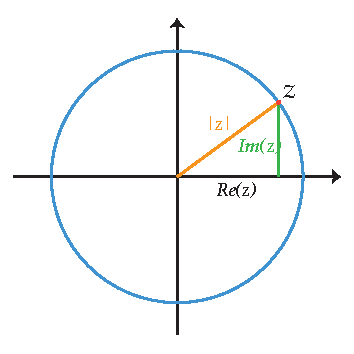
\includegraphics[scale=1.3]{Bilder/Einheitskreis.pdf}
\]
jetzt: $z= e^{ix} := \exp (ix)$ Dann
\begin{align*}
		| e^{ix} | &= \sqrt{e^{ix} \overline{e^{ix}}} \\
		&= \sqrt{ e^{ix} e^{\overline{ix}}} \\
		&= \sqrt{e^{ix} e^{-ix}} = e^0 = 1
\end{align*}
% subsection geometrische_interpretation (end)
% section die_komplexen_zahlen (end)

\section{Winkelfunktion} % (fold)
\label{sec:winkelfunktion}

\subsection{Definition} % (fold)
\label{sub:definition}
Wir definieren Funktionen
\begin{enumerate}[(i)]
	\item $ \cos : \mathds{R} \to \mathds{R} \quad  x \mapsto \re (e^{ix})$
	\item $\sin : \mathds{R} \to \mathds{R} \quad x \mapsto \im (e^{ix})$
\end{enumerate}
% subsection definition (end)

\subsection{Bemerkung} % (fold)
\label{sub:bemerkung}
\begin{enumerate}[(i)]
	\item $e^{ix}= \cos x + i \sin x$ (Euler'sche Formel)
	\item $\cos x , \sin x \in [-1, 1] $ für alle $x \in \mathds{R}$, da $| \re(e^{ix}) | , | \im(e^{ix})| \le |e^{ix}| =1$
\end{enumerate}
% subsection bemerkung (end)

\subsection{Proposition} % (fold)
\label{sub:proposition}
$\forall x\in \mathds{R}: $
\begin{enumerate}[(i)]
	\item $\cos x = \frac{1}{2} ( e^{ix} + e^{-ix}) $
	\item $\sin x = \frac{1}{2i} ( e^{ix} - e^{-ix}) $
	\item $\cos(-x) =  \cos x$
	\item $\sin (-x) = - \sin x $
	\item $\cos^2 x + \sin^2 x = 1$
\end{enumerate}
\underline{\textbf{Beweis:}} \\
(ii) \begin{align*}
	z-\overline{z} &= \re(z) + i \im(z) - \Big( \re(z) - i \im(z) \Big) \\
	&= 2i \im(z)
\end{align*}
(iii)
\begin{align*}
	\cos(-x) &= \re(e^{-ix}) \overset{\text{10.12}}{=} \re \left(\overline{e^{ix}}\right) \\
	&= \re(e^{ix}) \\
	&= \cos x
\end{align*}
(v)
\begin{align*}
	\cos^2 x + \sin^2 x &= (\re(e^{ix}))^2 + (\im(e^{ix}))^2 \tag{Definition des Betrags}\\
	&= | e^{ix} | ^2  \\&= 1
\end{align*}
% subsection proposition (end)

\subsection{Satz} % (fold)
\label{sub:satz}
$\cos , \sin : \mathds{R} \to [-1,1] $ sind stetig.
\vspace{\baselineskip} \\
\underline{\textbf{Beweis:}} \\
Sei $x_0 \in \mathds{R}$. Sei $\varepsilon >0$ gegeben. $\exp  : \mathds{C} \to \mathds{C}$ ist stetig, daher existiert $\delta >0$, so dass gilt:
\[
	z \in \mathds{C}, |z- ix_0 | < \delta \Longrightarrow  | \exp (z) - \exp (ix_0) | < \varepsilon 
\]
Sei $x \in \mathds{R}$ ein Punkt mit $|x-x_0| < \delta$. Dann gilt:
\[
	|\underbrace{ix}_{z} -ix_0 | = |i| \cdot |x-x_0|  =|x-x_0| < \delta 
\]
und wir erhalten
\begin{align*}
		| \cos x - \cos x_0 | &= |\re(e^{ix}) - \re(e^{ix_0}) | \\
		&= | \re(e^{ix} - e^{ix_0})| \\
		&\le | e^{ix} - e^{ix_0}| \\
		&< \varepsilon
\end{align*}
[bzw. mit 11.3] \hfill \( \square \)
% subsection satz (end)

\subsection{Satz: Additionstheoreme} % (fold)
\label{sub:satz_additionstheoreme}
$\forall x,y \in \mathds{R} : $ 
\begin{align*}
	\cos (x+y)  &= \cos x \cos y - \sin x \sin y \\
	\sin (x+y) &= \cos x \sin y + \sin x \cos y
\end{align*}
\underline{\textbf{Beweis:}} 
\begin{align*}
	\cos (x+y) + i \sin (x+y) = e^{i(x+y)} &= e^{ix} e^{iy} \\
	&= (\cos x + i \sin x) ( \cos y + i \sin y) \\
	&= \cos x \cos y - \sin x \sin y + i (\cos x \sin y + \sin x \cos y)
\end{align*}
% subsection satz_additionstheoreme (end)

\subsection{Corollar} % (fold)
\label{sub:corollar}
$\forall x,y \in \mathds{R}:$
\begin{align*}
	\sin x - \sin y = 2 \cos \left(\frac{x+y}{2}\right) \sin \left(\frac{x-y}{2} \right) \\
	\cos x - \cos y = -2 \sin \left(\frac{x+y}{2} \right) \sin \left( \frac{x-y}{2} \right)
\end{align*}
\underline{\textbf{Beweis:}} \\
Setze $u:= \frac{x+y}{2} $ , $v:= \frac{x-y}{2} $, dann
\[
	x= u+v \quad , \quad y= u-v
\]
\begin{align*}
	\sin x - \sin y &= \sin (u+v) - \sin (u-v) \\
	&= \cos u \sin v + \sin u \cos v - (\sin u \cos (-v) + \cos u \sin (-v)) \\
	&= 2 \cos u \sin v \\
	&= 2 \cos \left(\frac{x+y}{2} \right) \sin \left(\frac{x-y}{2} \right)
\end{align*}
% subsection corollar (end)

\subsection{Satz} % (fold)
\label{sub:satz}
Für $x \in \mathds{R}$ gilt: 
\[
	\cos x = \sum\limits_{k=0}^{\infty} (-1)^k \frac{x^{2k}}{(2k)!} = 1 - \frac{x^2}{2!} + \frac{x^4}{4!} - \frac{x^6}{6!} \pm \ldots      
\]
\[
	\sin x = \sum\limits_{k=0}^{\infty} (-1)^k \frac{x^{2k+1}}{(2k+1)!} = x - \frac{x^3}{3!}  + \frac{x^5}{5!} - \frac{x^7}{7!}  \pm \ldots 
\]
Die Reihen konvergieren absolut.
\vspace{10pt} \\
Weiter gilt
\begin{align*}
	\cos x &= \sum\limits_{k=0}^{n} (-1)^k \frac{x^{2k}}{(2k)!}  + r_{2n+2} (x) \\
	\sin x &= \sum\limits_{k=0}^{n} (-1)^k \frac{x^{2k+1}}{(2k+1)!} + r_{2n+3}(x)  
\end{align*}
wobei $|r_m(x)|\le \frac{|x|^m}{m!} $ falls $|x| \le m+1$ , $m=2n+2 , 2n+3$
\vspace{\baselineskip} \\
\underline{\textbf{Beweis:}} \\
\begin{itemize}
	\item \underline{absolute Konvergenz:} \\
	$\exp (x)$ ist Majorante \hfill \( \square \)
	\item 
	\begin{align*}
		\cos x = \re(e^{ix}) &= \re \left(\lim\limits_{n \to \infty} \sum\limits_{k=0}^{n} \frac{(ix)^k}{k!} \right) \\
		&= \re \left( \lim\limits_{n \to \infty}  \left( \sum\limits_{k=0}^{2n+1} \frac{ (ix)^k}{k!} \right) \right) \\
		&= \re \left(\lim\limits_{n \to \infty}  \left( \sum\limits_{k=0}^{n} \frac{(ix)^{2k}}{(2k)!} +
		 \sum\limits_{k=0}^{n} \frac{(ix)^{2k+1}}{(2k+1)!}    \right)\right) \\
		&= \lim\limits_{n \to \infty} \re \left(\sum \ldots + \sum \ldots \right)  \tag{10.3} \\
		&= \lim\limits_{n \to \infty} \left( \re \left( \sum\limits_{k=0}^{n} \frac{i^{2k} x^{2k}}{(2k)!} +
		\sum\limits_{k=0}^{n} \frac{i^{2k+1} x^{2k+1}}{(2k+1)!}    \right) \right) \\
		&= \lim\limits_{n \to \infty} \left(\re \left( \underbrace{\sum\limits_{k=0}^{n} \frac{(-1)^k x^{2k}}{(2k)!}}_{\in \mathds{R}} + 
				i \underbrace{\sum\limits_{k=0}^{n} \frac{(-1)^k x^{2k+1}}{(2k+1)!}}_{\in \mathds{R}}    \right) \right) \\
		&= \lim\limits_{n \to \infty} \left( \sum\limits_{k=0}^{n} \frac{(-1)^k x^{2k}}{(2k)!}  \right) 
	\end{align*}
	ebenso für $\sin x$
	\item \underline{Restglied:} \\
	\begin{align*}
		|r_{2n+2} (x)| &= \left| \sum\limits_{k=0}^{\infty} (-1)^k \frac{x^{2k}}{(2k)!} \right| \\
		&= \left| \frac{x^{2n+2}}{(2n+2)!} \right| \cdot  | ( 1 - a_1 + a_2 - a_3 + \ldots ) |  
	\end{align*}
	wo $0 \le a_k = a_{k-1} \frac{x^2}{(2n + 2k +1)(2n+2k+2)} \underset{|x| \le 2n+2+1}{\le} a_{k-1}, $ mit $k\ge 1$ (durch simples Anstarren!)
	\vspace{10pt} \\
	Es gilt
	\[
		 0 \le (\underbrace{1- a_1}_{\ge 0} + \underbrace{a_2- a_3}_{\ge 0} + \underbrace{a_4 - a_5}_{\ge 0} + \ldots ) \le 1
	\]
	Es folgt
	\[
		| r_{2n+2}(x) | \le \frac{|x|^{2n+2}}{(2n+2)!} \enspace , \quad m=2n+3 \text{ analog} 
	\]
	\hfill \( \square \)
\end{itemize}
% subsection satz (end)

\subsection{Proposition} % (fold)
\label{sub:proposition}
\[
	\cos (2) \le - \frac{1}{3} 
\]
\underline{\textbf{Beweis:}} \\
	\[
		\cos(2) = 1- \frac{2^2}{2} + r_4 (2) 
		= -1 + r_4 (2)
	\]
\begin{align*}
	| r_4 (2)| &\le \frac{2^4}{4!} = \frac{2}{3} \quad \Rightarrow \quad \cos (2) \le - \frac{1}{3}   
\end{align*}
\hfill \( \square \)
% subsection proposition (end)

\subsection{Proposition} % (fold)
\label{sub:proposition}
\[
	\forall x \in (0,2] : \sin x > 0
\]
\underline{\textbf{Beweis:}} \\
\begin{align*}
	\sin x = x + r_3 (x)
\end{align*}
\begin{align*}
	| r_3 (x) | < \frac{|x|^3}{3!} = |x| \frac{|x|^2}{3 \cdot 2} < |x|  \quad \Rightarrow \quad \sin x > 0
\end{align*}
% subsection proposition (end)

\subsection{Propostion} % (fold)
\label{sub:propostion}
$\cos$ ist auf $[0,2]$ streng monoton fallend.
\vspace{10pt} \\
\underline{\textbf{Beweis:}} \\
Sei $0 \le y \le x \le 2$. 
\begin{align*}
	\cos x - \cos y &= - 2 \underbrace{\sin \left( \frac{x+y}{2} \right)}_{>0} \underbrace{\sin \left(\frac{x-y}{2} \right)}_{>0}  < 0\tag{11.6 und 11.9} \\
	&\Rightarrow \cos \text{ auf } [0,2] \text{ streng monoton fallend }
\end{align*}

% subsection propostion (end)

\subsection{Definition und Satz} % (fold)
\label{sub:definition}
$\cos$ hat in $(0,2)$ genau eine Nullstelle. Das Zweifache dieser Nullstelle nennen wir $\pi$.
\vspace{\baselineskip} \\
\underline{\textbf{Beweis:}} \\
\begin{align*}
	\cos (0) &= \re (e^{i0}) -1 \quad  , \quad  \cos (2) < - \frac{1}{3} \\
	\cos \text{ stetig } &\Rightarrow  \exists \text{ Nullstelle in } (0,2) \\
	\cos \text{ ist streng monoton fallend } &\Rightarrow \exists! \text{ Nullstelle}
\end{align*}
\hfill \( \square \)
% subsection definition (end)

\subsection{Bemerkung} % (fold)
\label{sub:bemerkung}
\begin{enumerate}[(i)]
	\item \begin{itemize}
		\item $e^{i \frac{\pi}{2} } = i$
		\item $e^{i \pi} = -1$ \quad (Eulersche Identität)
		\item $e^{i \frac{3 \pi}{2}}= -i$
		\item $e^{2 \pi i} = 1$
	\end{itemize}
	\underline{\textbf{Beweis:}} \\
	\begin{enumerate}[(i)]
		\item 
		\[
			\re ( e^{i \frac{\pi}{2} })  =\cos \frac{\pi}{2} = 0 \quad | e^{i \frac{\pi}{2} } | = 1
			\Rightarrow \im ( e^{i \frac{\pi}{2} })^2 = 1 
		\]
		$\im ( e^{i \frac{\pi}{2} }) = \sin \frac{\pi}{2} > 0 $ Rest: Funktionalgleichung
	\end{enumerate}
	\item 
	\begin{itemize}
		\item $\cos (x + 2 \pi) = \cos x $
		\item $\sin ( x + 2 \pi) = \sin x$
	\end{itemize} da $e^{ix} = e^{i(x+2\pi)}$
	\begin{itemize}
		\item $\cos (x + \pi) = - \cos x$
		\item $\sin (x + \pi) = - \sin x$
	\end{itemize}
	da $e^{ix}= - e^{i (x+\pi)}$
	\begin{itemize}
		\item $\cos (x +\frac{\pi}{2} ) = - \sin x$
		\item $\sin ( x + \frac{\pi}{2} ) = \cos x$
	\end{itemize}
	da
	\begin{align*}
		\cos \left( x+ \frac{\pi}{2}  \right) + i sin \left( x + \frac{\pi}{2} \right) &= e^{i(x+\frac{\pi}{2} )} \\
		&= e^{ix} \cdot e^{i \frac{\pi}{2} } = e^{ix} \cdot i = (\cos x + i \sin x) \cdot  i \\
		&= - \sin x + i \cos x
	\end{align*}
	Es genügt daher, das Verhalten von $\cos$ auf $[0, \frac{\pi}{2} ]$ zu kennen.
	\item Für die Nullstellen gilt
	\[
		\{  x \in \mathds{R} \mid \cos x = 0 \} = \left\{ \frac{\pi}{2} + k \cdot \pi \mid k \in \mathds{Z} \right\}
	\]
	\[
		\{ x \in \mathds{R} \mid \sin x = 0 \} = \{ k \cdot \pi \mid k \in \mathds{Z}\}
	\]
	\underline{\textbf{Beweis:}} \\
	\begin{align*}
		0 &= \cos \frac{\pi}{2} = {-1}^k \cos (\frac{\pi}{2} + k \cdot  \pi ) \\
		&\Rightarrow  \text{ für } k \in \mathds{Z} \text{ ist } \frac{\pi}{2} + k \cdot \pi \text{ Nullstelle von } \cos
	\end{align*}
	11.11 $\Rightarrow \cos$ hat keine Nullstellen in $[0, \frac{\pi}{2})$
	\[
		\cos x = \cos (-x) \enspace \Rightarrow \enspace \cos \text{ hat keine Nullstelle in } \left(- \frac{\pi}{2} , \frac{\pi}{2}\right)
	\]
	$\cos (x+ k \cdot \pi)= (-1)^k \cos x \Rightarrow \cos$ hat keine Nullstellen in $ \left( k \cdot \pi - \frac{\pi}{2} , k \cdot \pi + \frac{\pi}{2} \right) $. 
	Nullstellen von $\sin$ analog. 
	\item 
	\[
		\forall x \in \mathds{R} : \underbrace{e^{ix}= 1}_{\Leftrightarrow \sin x = 0 \text{ und } \cos x \ge 0} 
		\Leftrightarrow x=k \cdot 2 \pi \text{ für ein } k \in \mathds{Z}
	\]
	\item $\cos$ ist auf dem $[0, \pi ]$ streng monoton fallend und auf $[\pi , 2 \pi ]$ streng monoton wachsend.
	\vspace{10pt} \\
	$\sin$ ist auf $[- \frac{\pi}{2} , \frac{\pi}{2}]$ streng monoton wachsend und auf $[\frac{\pi}{2} , \frac{ 3 \pi}{2}]$ streng monoton fallend.
	\vspace{\baselineskip} \\
	\underline{\textbf{Beweis:}} \\
	$\cos$ streng monoton fallend auf $[0, \frac{\pi}{2}]$ nach 11.11
	\[
		\cos x = - \cos (x - \pi ) = \underbrace{- \underbrace{\cos (\pi  -x)}_{\text{streng monoton wachsend auf } [\frac{\pi}{2} , \pi ]}}
		_{\text{streng monoton fallend auf } [\frac{\pi}{2}, \pi ]}
	\]
	\[
		\cos x \begin{cases}
			\ge 0, & x \in [0, \frac{\pi}{2}]\\
			\le 0 , & x \in [\frac{\pi}{2} ,\pi ]
			
		\end{cases}
	\]
	$\Rightarrow \cos $ streng monoton fallend auf $[0, \pi ]$ \hfill \( \square \)
	\vspace{\baselineskip} \\
	\[
		\cos 0 = 1 \quad \cos \pi = -1 \qquad \sin - \frac{\pi}{2} = -1 \quad \sin \frac{\pi}{2}= 1
	\]
	stetig auf Intervallen
	\vspace{10pt} \\
	$\Rightarrow \cos : [0, \pi ] \to [-1 ,1]$ besitzt stetige Umkehrfunktion 
	\[
		\arccos : [-1,1] \to [0, \pi ] 
	\]
	$\sin : [- \frac{\pi}{2} , \frac{\pi}{2}] \to [-1,1]$ besitzt stetige Umkehrfunktion
	\[
		\arcsin : [-1,1] \to [ - \frac{\pi}{2} , \frac{\pi}{2}] 
	\]
	\item 
	\[
		\includegraphics[scale=0.8]{Bilder/Sine_cosine_one_period.pdf}
	\]
\end{enumerate}

% subsection bemerkung (end)

\subsection{Satz: Polarzerlegung} % (fold)
\label{sub:satz_polarzerlegung}
\[
	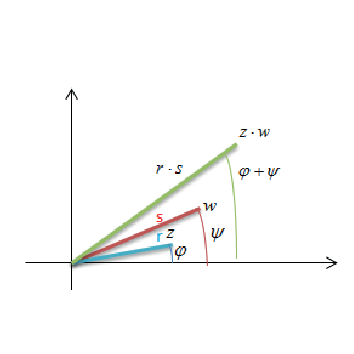
\includegraphics[scale=1]{Bilder/polarzerlegung.pdf}
\]
Jedes $0 \not= z \in \mathds{C}$ lässt sich eindeutig in der Form 
\[
	z= r \cdot e^{i \varphi} \quad , \enspace r>0 \enspace , \enspace \varphi \in [0, 2 \pi )
\]
schreiben. Insbesondere gilt: Die Abbildung 
\[
	[0, 2 \pi ) \to \{ z \mid |z| =1\} \subset \mathds{C}
\]
ist bijektiv.
\vspace{\baselineskip} \\
\underline{\textbf{Beweis:}} \\
Setze $r := |z|$ und $w := \frac{z}{r} $, dann $|w| = \left| \frac{z}{r} \right| =  \frac{|z|}{|r|}  = 1$ und $\re (w) \in [-1, 1]$. Setze
\[
	\varphi := \begin{cases}
		\arccos \big(\re (w)\big) \in [0, \pi ], &\text{ falls }\im (w) \ge 0\\
		\arccos \big( - \re(w)\big)+ \pi \in (\pi , 2 \pi ), &\text{ falls }\im (w) < 0
	\end{cases}
\]
Dann gilt

\begin{align*}
	e^{i \varphi} &= \cos \varphi + i \sin \varphi \\
	&= \begin{cases}
		\re (w) + i \im (w), &\text{ falls }\varphi \in [0, \pi ],  \im w \ge 0\\
		\re (w) + i \im (w),  &\text{ falls } \varphi \in(\pi , 2 \pi) , \im (w)< 0 
	\end{cases} \\
	&= w
\end{align*}
\hrule 
\vspace{5pt} 
Nebenrechnung:
\[
	\cos ( \arccos ( - \re (w)) + \pi ) = - \cos ( \arccos (- \re (w))) = - (- \re(w)) = \re w
\]
\hrule
$\Rightarrow r \cdot  e^{i \varphi} = r \cdot w = z$ \\
Eindeutigkeit: Sei $z= r \cdot e^{i \varphi}= s \cdot e^{i \psi}$, wo $r,s >0$ und $\varphi, \psi \in [0, 2 \pi )$ 
\[
	\Rightarrow r =|r| \cdot \left| e^{i \varphi} \right|=|z| = |s| \cdot \left| e^{i \psi} \right| = s
\]
$1= \frac{z \overline{z}}{r \cdot s}= e^{i \varphi} \cdot e^{- i \psi} = e^{i(\varphi - \psi)}  $\\
 $\varphi - \psi \overset{11.12}{=} k \cdot 2 \pi $ für ein $k \in \mathds{Z}$ , $\varphi, \psi \in [0, 2 \pi ) \Rightarrow k =0 \Rightarrow \varphi = \psi$ \hfill \( \square \)
% subsection satz_polarzerlegung (end)

\subsection{Bemerkung} % (fold)
\label{sub:bemerkung}
$z= r \cdot e^{i \varphi}, w= s \cdot e^{i \psi}$ dann
\[
	z \cdot w = r \cdot s \cdot e^{i(\varphi + \psi)}
\]
"'Beträge multiplizieren, Winkel addieren"'
% subsection bemerkung (end)

\subsection{Corollar} % (fold)
\label{sub:corollar}
Für $n \in \mathds{N}^*$ besitzt die Gleichung $z^n =1$ genau $n$ Lösungen, $e^{i \frac{2 \pi k}{n} }$ , $k = 0,1, \ldots , n-1$
\vspace{\baselineskip} \\
\underline{\textbf{Beweis:}} \\
$e^{i \frac{2 \pi  k}{n} }$ ist Lösung für $k=0, 1, \ldots , n-1$. Sei nun $z$ eine Lösung. Dann $z= r e^{i \varphi}$ , $r= |z|=1$ . 
\[
	2 = z^n = e^{i \varphi n} \Rightarrow  \varphi \cdot n = k \cdot 2 \pi \text{ für ein } k \in \mathds{Z}
\]
$\Rightarrow \varphi = \frac{2 \pi  k}{n} $ für eine $k \in \mathds{Z}$ , $0 \le k \le n-1$
% subsection corollar (end)
% section winkelfunktion (end)
\newpage
\section{Differentiation} % (fold)
\label{sec:differentiation}

\subsection{Definiton} % (fold)
\label{sub:definiton}
Sei $D \subset \mathds{R}$ , $f : D \to \mathds{R}$ eine Funktion und $\overline{x} \in D$ ein Punkt, so dass eine Folge in $D$ mit Limes $\overline{x}$ existiert.\\
$f$ heißt differenzierbar in $\overline{x}$ falls der Limes 
\[
	f'(\overline{x}) := \lim\limits_{\substack{x \to \overline{x} \\ x \in D \backslash \{\overline{x} \} }} \frac{f(x)- f(\overline{x})}{x- \overline{x}} \in \mathds{R}
\]
existiert. $f'(\overline{x})$ heißt Ableitung von $f$ im Punkt $\overline{x}$, wir schreiben auch 
\[
	\frac{df}{dx}(\overline{x}) \quad , \quad Df(\overline{x}) 
\]
d.h. für jede Folge $(x_n)_{n \in \mathds{N}} \subset D \backslash \{ \overline{x} \}$ mit $x_n \xrightarrow{n \to \infty} \overline{x}$, konvergiert
\[
	\left(  \frac{ f(x_n)- f(\overline{x}) }{x_n - \overline{x}} \right)_{n \in \mathds{N}}
\] 
gegen ein und denselben Grenzwert.
% subsection definiton (end)

\subsection{Bemerkung} % (fold)
\label{sub:bemerkung}
\begin{enumerate}[(i)]
	\item Falls $D \subset \mathds{R}$ ein echtes Intervall ist, so existiert für jedes $\overline{x} \in D$ eine Folge in $D$ mit Limes $\overline{x}$.
	\item Falls $f$ in $\overline{x}$ differenzierbar ist, so gilt 
	\[
		f'(\overline{x})= \lim\limits_{\substack{h \to 0 \\ h \not= 0 \\ (\overline{x} +h \in D)}} \frac{f(\overline{x} +h) - f(\overline{x})}{h}
	\]
	\item 
	\[
		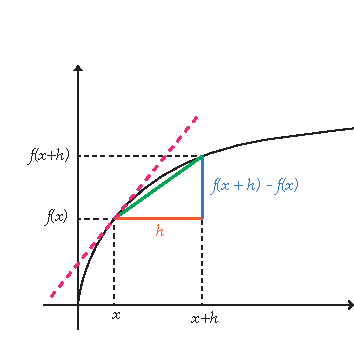
\includegraphics[scale=1.5]{Bilder/Ableitung.pdf}
	\]
	\item $D, f, \overline{x}$ wie in 12.1 \\
	$f$ differenzierbar in $\overline{x}$, genau dann, wenn $\varphi : D \to \mathds{R}$ existiert mit 
	\begin{enumerate}[ a)]
		\item $\varphi$ ist stetig in $\overline{x}$
		\item $f(x)= f(\overline{x})+ (x-\overline{x}) \varphi(x)$ , $x \in D$
	\end{enumerate}
\underline{\textbf{Beweis:}} \\
$\Leftarrow$ Übung! \\
$\Rightarrow $ Übung mit 
\[
	\varphi(x) := \begin{cases}
		\frac{f(x)- f(\overline{x})}{x- \overline{x} } , &\text{ falls } x \in D \backslash \{ \overline{x} \}\\
		f'(\overline{x}) , &\text{ falls } x = \overline{x}
	\end{cases}
\]
\end{enumerate}
% subsection bemerkung (end)

\subsection{Beispiel} % (fold)
\label{sub:beispiel}
\begin{enumerate}[(i)]
	\item $f(x)= x^n$ ( $n \in \mathds{N} $) ist auf $\mathds{R}$ differenzierbar. \\
	$n \in \mathds{N}^*$ : 
	\[
		\frac{f(x) - f(\overline{x})}{x -\overline{x}} = \frac{x^n - \overline{x}^n}{x- \overline{x}} = x^{n-1} + x^{n-2} \overline{x} + \ldots + x \overline{x}^{n-2}
		+ \overline{x}^{n-1}  
	\]
	$x \to \overline{x} : \quad n \cdot \overline{x}^{n-1}$ 
	\vspace{10pt} \\
	$n=0$ : 
	\[
		\frac{f(x)- f(\overline{x})}{x- \overline{x}} = \frac{1-1}{x- \overline{x}} = 0 \to 0  
	\]
	\item $f(x)=e^x$
	\[
		\frac{f(\overline{x} +h) - f(\overline{x})}{h} = \frac{e^{\overline{x}+h} - e^{\overline{x}}}{h} 
		= e^{\overline{x}} \cdot \frac{e^h -1}{h} \underset{\text{wegen 9.25 (v)}}{\xrightarrow{h \to 0}} e^{\overline{x}}   
	\]
	\item $f(x)=x ^{-1}$ ist auf $\mathds{R} \backslash \{0\}$ differenzierbar
	\begin{align*}
		\frac{f( \overline{x} +h)- f(\overline{x})}{h} &= \frac{1}{h} (\frac{1}{\overline{x}+h} - \frac{1}{x}  ) \\
		&= \frac{1}{h} \frac{\overline{x} - (\overline{x} +h)}{(\overline{x} +h) \overline{x}} \\
		&= - \frac{1}{(\overline{x} +h) \overline{x}} \xrightarrow{h \to 0} - \frac{1}{\overline{x}^2} = f' (\overline{x})     
	\end{align*}
	\item $f(x)= \sin{x}$
	\begin{align*}
				\lim\limits_{\substack{h \to 0 \\ h \not= 0}} \frac{\sin h}{h}-1 &=   \lim\limits_{\substack{h \to 0 \\ h \not= 0}} \frac{\sin h -h}{h} \\
				&= \lim\limits_{\substack{h \to 0 \\ h \not= 0}} \frac{h + r_3(h) -h}{h} \\
				&= \lim\limits_{\substack{h \to 0 \\ h \not= 0}} \frac{r_3(h)}{h}  =0
	\end{align*}
	Restgliedabschätzung:
	\[
		\left| \frac{r_3(h)}{h} \right| = \frac{|r_3(h)|}{|h|} \le \frac{\frac{|h|^3}{3!} }{|h|} = \frac{|h|^2}{6}   \quad \text{für } |h|\le 4 
	\]
	Es folgt (mit den Additionstheoremen 11.6)
	\begin{align*}
		\lim\limits_{\substack{h \to 0 \\ h \not= 0}} \frac{\sin (\overline{x} +h) - \sin ( \overline{x})}{h} &= \lim\limits_{\substack{h \to 0 \\ h \not= 0}} 
		\frac{2 \cos (\frac{\overline{x} +h + \overline{x}}{2}) \sin (\frac{\overline{x} +h - \overline{x}}{2} )}{h} \\
		&= \lim\limits_{\substack{h \to 0 \\ h \not= 0}} \cos \left(\frac{ \overline{x} + h + \overline{x}}{2} \right) \lim\limits_{\substack{h \to 0 \\ h \not= 0}} 
		\frac{\sin ( \frac{\overline{x} + h - \overline{x}}{2} )}{\frac{h}{2} } \\
		&= \lim\limits_{\substack{h \to 0 \\ h \not= 0}} \cos \left(\overline{x} + \frac{h}{2} \right) \lim\limits_{\substack{h \to 0 \\ h \not= 0}} 
		\frac{\sin \frac{h}{2} }{\frac{h}{2} } \\
		&= \cos (\overline{x}) \cdot 1 = \cos \overline{x} = \sin' (\overline{x})
	\end{align*}
	\item Analog: $\cos'(\overline{x})= - \sin (\overline{x})$ , $\overline{x } \in \mathds{R}$
\end{enumerate}
% subsection beispiel (end)

\subsection{Satz} % (fold)
\label{sub:satz}
$f,g: D \to \mathds{R}$ differenzierbar in $\overline{x} \in D$ , $\lambda , \mu \in \mathds{R}$. Dann sind $\lambda f + \mu g$ und $f \cdot g$ differenzierbar in $\overline{x}$ und 
\begin{align*}
	(\lambda \cdot f + \mu \cdot g)' (\overline{x}) &= \lambda  \cdot f'(\overline{x}) + \mu \cdot g'(\overline{x}) \\
	(f \cdot g)' (\overline{x}) &= f'(\overline{x}) \cdot g(\overline{x})+ f(\overline{x}) \cdot g'(\overline{x})
\end{align*}
Falls $g(x)\not= 0$ für alle $x \in D$, so ist $\frac{f}{g} $ in $\overline{x}$ differenzierbar mit 
\[
	\left( \frac{f}{g} \right)' (\overline{x}) = \frac{ f' (\overline{x}) g(\overline{x}) - f(\overline{x}) g'(\overline{x})}{g(\overline{x})^2} 
\]
\underline{\textbf{Beweis:}} \\
\begin{align*}
	&\frac{(\lambda \cdot f + \mu \cdot g)(\overline{x} +h ) - (\lambda \cdot f + \mu \cdot  g)(\overline{x} )}{h}\\
	&= \lambda \frac{f(\overline{x}  +h )- f(\overline{x} )}{h} + \mu \frac{g(\overline{x}  +h) - g(\overline{x} )}{h} \\
	&\xrightarrow{h \to 0}  \lambda f'(\overline{x} ) + \mu g' (\overline{x} ) 
\end{align*}
\begin{align*}
  \frac{(fg) (\overline{x}  + h) - (fg)(\overline{x} )}{h} &= \frac{f(\overline{x}  +h) g(\overline{x} +h) - f(\overline{x}) g(\overline{x} )}{h}  \\
 &=  \frac{f(\overline{x} +h)- f(\overline{x} )}{h} \cdot g(\overline{x} +h) + f(\overline{x}) \cdot \frac{g(\overline{x} +h) - g(\overline{x})}{h}  \\
 &\xrightarrow{h \to 0}  f'(\overline{x}) \cdot g(\overline{x})+ f(\overline{x}) g'(\overline{x})
\end{align*}
Haben benutzt: $g$ ist stetig in $\overline{x} $ nach Übung. (nach 12.2(iv) gilt
\[
	g(x)= g(\overline{x})+ (x-\overline{x}) \varphi(x)
\] 
mit $\varphi : D \to \mathds{R}$ stetig in $\overline{x}$)
\begin{align*}
	\frac{\frac{f}{g}( \overline{x} +h) - \frac{f}{g} (\overline{x})}{h} &= \frac{1}{g(\overline{x} +h) g(\overline{x})} 
	\left( \frac{(f(\overline{x} +h)-f(\overline{x})) g(\overline{x})}{h} - \frac{f(\overline{x}) (g(\overline{x} +h)-g(\overline{x}))}{h}   \right) \\
	& \xrightarrow{h \to 0} \frac{1}{g(\overline{x})^2} \cdot  \left( f'(\overline{x}) \cdot g(\overline{x}) - f(\overline{x}) g'(\overline{x}) \right)   
\end{align*}
% subsection satz (end)

\subsection{Beispiel} % (fold)
\label{sub:beispiel}
\begin{enumerate}[(i)]
	\item $f(x)=x^{-n}= \frac{1}{x^n} $, $n \in \mathds{N}$
	\[
		f'(x)= \frac{0 \cdot x^n- 1 \cdot n \cdot x^{n-1}}{(x^n)^2} = -n \cdot x^{n-1-2n} = -n x^{-n-1} 
	\]
	also $\frac{dx^k}{dx} =k x^{k-1} $ für alle $k \in \mathds{Z}$
	\item $\tan : (- \frac{\pi}{2}, \frac{\pi}{2}) \to \mathds{R}$ definiert durch $\tan(x)= \frac{\sin x}{\cos x} $
	\[
		\tan' (x) = \frac{\cos x \cdot \cos x - \sin x \cdot (- \sin x)}{\cos^2 x} = \frac{1}{\cos^2 x} 
	\]
\end{enumerate}
% subsection beispiel (end)

\subsection{Satz} % (fold)
\label{sub:satz}
$I \subset \mathds{R}$ echtes Intervall, $f : I \to \mathds{R}$ stetig und streng monoton. Sei $g : f(I) \to I$ die Umkehrfunktion (9.18). \\
Falls $f$  in $\overline{x} \in I$ differenzierbar ist mit $f'(\overline{x}) \not= 0$, so ist $g$ in $f(\overline{x}) \in f(I)$ differenzierbar mit 
\[
	g'\big( f(\overline{x}) \big) = \frac{1}{f'(\overline{x})}
\]
Falls also $f$ in $I$ differenzierbar ist mit $f'(x) \not= 0$ für alle $x \in I$, so ist $g$ differenzierbar in $f(I)$ und 
\[
	g'(y) = \frac{1}{f'\big( g(y) \big)} \quad , \quad y \in f(I) 
\]
\underline{\textbf{Beweis:}} \\
Wollen: 
\[
	\lim\limits_{\substack{y \to f(\overline{x}) \\ y \not= f(\overline{x})}} \frac{g(y)- g(f(\overline{x}))}{y-f(\overline{x})}  
\]
Sei $(y_n)_{n \in \mathds{N}} \subset f(I) \backslash \{ f(\overline{x}) \}$ eine Folge mit $\lim\limits_{n \to \infty} y_n= f(\overline{x})=: \overline{y}$. \\
$g$ ist stetig nach 9.18, also
\[
	\overline{x} = g \circ f (\overline{x})= g(\overline{y}) = g \left( \lim\limits_{n \to \infty} y_n\right) = \lim\limits_{n \to \infty} g( y_n)
\] $g(y_n) \not= g(\overline{y})$ da $g$ bijektiv
\begin{align*}
	g'(f(\overline{x})) = \lim\limits_{n \to \infty} \frac{g(y_n) -g(\overline{y})}{y_n -\overline{y}} &= 
	\lim\limits_{n \to \infty} \frac{1}{\frac{y_n - \overline{y}}{g(y_n)- g(\overline{y})}} \\
	&= \lim\limits_{n \to \infty} \frac{1}{\frac{f(g(y_n)) - f(g(\overline{y}))}{g(y_n)- g(\overline{y})} } \\
	&= \frac{1}{f'(g(\overline{y}))} \\
	&= \frac{1}{f'(\overline{x})}     
\end{align*}
\hfill \( \square \)
% subsection satz (end)

\subsection{Beispiel} % (fold)
\label{sub:beispiel}
\begin{enumerate}[(i)]
	\item $\ln' (y) = \frac{1}{\exp \big(\ln(y) \big) } = \frac{1}{y}  $
	\item Für $y \in (-1,1)$ gilt
	\[
		\arcsin'(y) = \frac{1}{\sin' ( \arcsin y)}  = \frac{1}{\cos ( \underbrace{\arcsin y}_{\in ( - \frac{\pi}{2}, \frac{\pi}{2})})} 
		= \frac{1}{\sqrt{1- \sin ^2 ( \arcsin y)} } = \frac{1}{\sqrt{1- y^2} }  
	\]
	Nebenrechnung $ x \in \left( - \frac{\pi}{2} , \frac{\pi}{2} \right)$:
	\begin{align*}
		\cos (x) = | \cos (x) | 
		= \sqrt{\cos^2 (x)} = \sqrt{1 - \sin^2 (x)}  
	\end{align*}
	\item $\arctan : (- \infty, \infty) \to ( - \frac{\pi}{2}, \frac{\pi}{2})$ \\
	Umkehrfunktion von tan. (Übung!)
	\[
		\arctan' (y) = \frac{1}{1+ y^2} 
	\]
\end{enumerate}
% subsection beispiel (end)

\subsection{Satz (Kettenregel)} % (fold)
\label{sub:satz_kettenregel_}
Seien $f : D \to \mathds{R}$ und $g : E \to \mathds{R}$ Funktionen mit $f(D) \subset E$. Falls $f$ in $\overline{x} \in D$ und $g$ in $f (\overline{x}) \in E$
differenzierbar sind, so ist $g \circ f$ differenzierbar in $\overline{x}$ und es gilt
\[
	(g \circ f)' (\overline{x}) = g' \left( f (\overline{x})\right) \cdot f' (\overline{x})
\]
\underline{\textbf{Beweis:}} \\
Sei $\overline{y}  := f(\overline{x} )$. Definiere $\varphi : E \to \mathds{R}$ durch
\[
	\varphi (y) := \begin{cases}
		\frac{g(y) - g(\overline{y})}{y- \overline{y} } , &\text{ falls }y \not= \overline{y} \\
		g'(\overline{y}) , &\text{ falls } y= \overline{y}  
	\end{cases}
\]
Dann ist $\varphi$ stetig in $\overline{y}$ und es gilt
\[
	g(y)- g(\overline{y} ) = \varphi (y) \cdot (y- \overline{y}) \quad , y \in E
\]
Wir erhalten
\begin{align*}
	\frac{g \circ f (x) - g \circ f (\overline{x} )}{x - \overline{x} } &= \frac{g \big( f(x) \big) - g \big( f(\overline{x}) \big)}{x - \overline{x}} \\
	&= \varphi ( f(x)) \frac{f(x) - f(\overline{x})}{x- \overline{x} }   \\
	\xrightarrow{x \to \overline{x}} & \underbrace{\varphi \big(f(\overline{x}) \big)}_{\substack{f \text{ stetig in } \overline{x} 
	\\ \varphi \text{ stetig in } f(\overline{x} )}}  \cdot f'(\overline{x})
	= g' \big( f(\overline{x})\big) \cdot f '(\overline{x})
\end{align*}
\hfill \( \square \)
% subsection satz_kettenregel_ (end)

\subsection{Beispiel} % (fold)
\label{sub:beispiel}
\begin{enumerate}[(i)]
	\item $a \in \mathds{R}$ $f: \mathds{R}_+^* \to \mathds{R}$ $x \mapsto x^a = \exp (a \ln x)$
	\begin{align*}
		f'(x) &= \exp' (a \ln x) \cdot \frac{d(a \ln x)}{dx} \\
		&= \exp (a \ln x) \cdot a \cdot x ^{-1} \\
		&= a x^{a-1} 
	\end{align*}
	\item allgemein:
	\[
		\frac{d \, e^{f(x)}}{dx} = f'(x) e^{f(x)} 
	\]
\end{enumerate}
% subsection beispiel (end)

\subsection{Definition} % (fold)
\label{sub:definition}
Sei $f : D \to \mathds{R}$ in $D$ differenzierbar. Dann ist $f' : D \to \mathds{R}$ eine Funktion. \\
Falls $f'$ in $D$ differenzierbar ist, so heißt $f$ in $D$ \underline{\textbf{zweimal differenzierbar}} und $f''(x) := (f')'(x)$. Wir schreiben auch $D^2 f(x)$, 
$\frac{d^2 f}{dx^2}(x) $ , $f^{(2)}(x)$.
\vspace{10pt} \\
$f$ heißt \underline{\textbf{$k$-mal differenzierbar}} in $D$, falls $f$ $(k-1)$-mal differenzierbar ist und $f^{(k-1)}$ differenzierbar ist. 
\[
	f^{(k)} (x) := \left( f^{(k-1)}\right)' (x) \enspace , \quad D^k f(x) \enspace , \quad \frac{d^k f}{d x^k} (x) 
\]
$f$ heißt \underline{\textbf{$\infty$-oft differenzierbar}} oder \underline{\textbf{glatt}}, falls $f$ $k$-mal diffrenzierbar ist für jedes $k \in \mathds{N}$
\[
	f^{(0)} (x) = f(x)
\]
% subsection definition (end)

\subsection{Beispiel} % (fold)
\label{sub:beispiel}
Polynome, $e^x$ , $\sin (x)$ , $\cos (x)$ , \ldots  sind glatt. 
\vspace{10pt} \\
\[
	f(x) := \begin{cases}
			x^2, &\text{ falls }x >0\\
			- x^2 , &\text{ falls } x < 0
		\end{cases}
\] 
ist 1-mal differenzierbar, aber nicht 2-mal denn $f'(x)= 2 |x|$
% subsection beispiel (end)

\subsection{Definition} % (fold)
\label{sub:definition}
$f : D \to \mathds{R}$ hat in $\overline{x} \in D$ ein \underline{\textbf{lokales Maximum (Minimum)}}, falls ein $\varepsilon >0$ existiert, so dass 
\[
	f(x) \underset{(\ge)}{\le} f(\overline{x}) \forall x \in D \cap (\overline{x} - \varepsilon , \overline{x} + \varepsilon)
\]
D.h.
\[
	f \mid_{D \cap (\overline{x} - \varepsilon , \overline{x} + \varepsilon)}
\]
besitzt Maximum (Minimum) in $\overline{x}$.
% subsection definition (end)

\subsection{Satz} % (fold)
\label{sub:satz}
$f : (a,b) \to \mathds{R}$ besitze in $\overline{x} \in (a,b)$ ein lokales \textbf{\underline{Extremum}} (d.h. Maximum oder Minimum) und sei in $\overline{x}$
differenzierbar. Dann gilt $f'(\overline{x})=0$.
\vspace{10pt} \\
\underline{\textbf{Beweis:}} \\
O.E.d.A besitzt $f$ in $\overline{x}$ ein lokales Maximum. \\
Dann existiert ein $\varepsilon >0$ so , dass $f(x) \le f(\overline{x})$ für alle $x \in (\overline{x} - \varepsilon, \overline{x} + \varepsilon)$. Es folgt
\begin{align*}
	0 \ge \underbrace{\lim\limits_{\substack{x \searrow \overline{x} \\ x \not= \overline{x} }} \frac{f(x) - f(\overline{x})}{x - \overline{x}}}_{f'(\overline{x})} &= 
	\lim\limits_{\substack{x \to \overline{x} \\ x \not= \overline{x} }} \frac{f(x) - f(\overline{x})}{x - \overline{x}} \\
	&= \lim\limits_{\substack{x \nearrow \overline{x} \\ x \not= \overline{x} }} \frac{f(x) - f(\overline{x})}{x - \overline{x}} \\
	&\ge 0
\end{align*}
\hfill \( \square \)
% subsection satz (end)

\subsection{Bemerkung} % (fold)
\label{sub:bemerkung}
$f'(\overline{x})=0$ ist notwendig, aber nicht hinreichend für Existenz eines lokalen Extremums. \\
zB $f(x)= x^3$ , $f'(0)=0$
% subsection bemerkung (end)

\subsection{Satz von Rolle} % (fold)
\label{sub:satz_von_rolle}
Sei $a < b$ und $f : [a,b] \to \mathds{R}$ stetig mit $f(a)= f(b)$. Sei $f$ in $(a,b)$ differenzierbar. \\
Dann exisitiet $\overline{x} \in (a,b)$ mit $f'(\overline{x})= 0$
\vspace{10pt} \\
\underline{\textbf{Beweis:}} \\
Trivial falls $f$ konstant. Andernfalls existiert ein $x_0 \in (a,b)$ mit $f(x_0) > f(a)$ oder $f(x_0)< f(a) = f(b)$. \\
$f$ stetig auf $[a,b]$ besitzt also Maximum und Minimum (nach 9.12). O.E. sei das Maximum von $f$ größer als $f(x_0)> f(a)= f(b)$. 
Das Maximum werde in $\overline{x} \in (a,b)$ angenommen. \\
$\Rightarrow f$ hat in $\overline{x} \in (a,b)$ ein lokales Maximum. \\
$\Rightarrow f'(\overline{x})=0$  
% subsection satz_von_rolle (end)

\subsection{Mittelwertsatz} % (fold)
\label{sub:mittelwertsatz}
Sei $a<b$ und $f : [a,b] \to \mathds{R}$ stetig. Sei $f$ in $(a,b)$ differenzierbar. Dann existiert ein $\overline{x} \in (a,b)$ mit 
\[
	\frac{f(b)- f(a)}{b-a} = f'(\overline{x}) 
\]
\underline{\textbf{Beweis:}} \\
Definiere: $F : [a,b] \to \mathds{R}$ durch $F(x)= f(x)- \frac{f(b)- f(a)}{b-a} \cdot (x-a) $. Dann ist $F$ stetig auf $[a,b]$ und differenzierbar auf $(a,b)$.
Außerdem gilt $F(a)=f(a)= F(b)$. \\
$\underset{\text{Rolle}}{\Rightarrow} $
\[
	\exists \enspace \overline{x} \in (a,b) \text{ mit } f'(\overline{x}) = \frac{f(b) - f(a)}{b-a} = F'(\overline{x}) = 0 
\]
\hfill \( \square \)
\[
	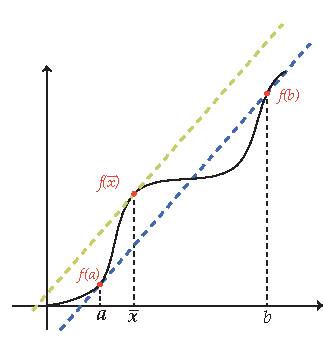
\includegraphics[scale=1]{Bilder/Mittelwertsatz.pdf}
\]
% subsection mittelwertsatz (end)

\subsection{Korollar} % (fold)
\label{sub:korolllar}
Sei $a<b$, $f : [a,b] \to \mathds{R}$ stetig auf $[a,b]$, differenzierbar auf $(a,b)$ mit $f'(x)=0$ für alle $x \in (a,b)$.\\
Dann ist $f$ konstant.
\vspace{10pt} \\
\underline{\textbf{Beweis:}} \\
Für $a \le x < y \le b$ gilt
\[
	\frac{f(y)- f(x)}{y-x} = f'(\overline{x}) = 0 \enspace \Rightarrow f(y)= f(x)
\]
für ein $\overline{x} \in (x,y)$ \hfill \( \square \)

% subsection korolllar (end)

\subsection{Korollar} % (fold)
\label{sub:Korollar}
Sei $\lambda \in \mathds{R}$ und $f : \mathds{R} \to \mathds{R}$ differenzierbar mit $f'(x)= \lambda \cdot f(x)$. Dann gilt
\[
	f(x)= f(0) \cdot e^{\lambda \cdot x}
\]
\underline{\textbf{Beweis:}} \\
Setze: $F(x) := f(x) \cdot  e^{- \lambda x}$, dann ist $F$ differenzierbar mit 
\[
	F'(x) = f'(x) \cdot e^{- \lambda x} + f(x) (- \lambda e^{- \lambda x}) = 0
\]
$\Rightarrow F$ ist konstant mit 
\[
	f(x) \cdot e^{- \lambda x}=F(x)= F(0)= f(0) 
\]
Multiplizieren mit $e^{- \lambda x}$ \hfill \( \square \)
% subsection corollar (end)

\subsection{Satz (l'Hospital)} % (fold)
\label{sub:satz}
Seien $f,g (a,b) \to \mathds{R}$ differenzierbar und $g'(x) \not= 0$ für alle $x \in (a,b)$. Es gelte entweder oder
\begin{enumerate}[a)]
	\item $\lim\limits_{x \searrow a}f(x) = \lim\limits_{x \searrow a} g(x) = 0  $
	\item $\lim\limits_{x \searrow a} f(x) = \lim\limits_{x \searrow a}g(x) = \infty $
\end{enumerate}
Falls $\lim\limits_{x \searrow a} \frac{f'(x)}{g'(x)} $ existiert, so auch $\lim\limits_{x \searrow a} \frac{f(x)}{g(x)} $ und 
\[
	\lim\limits_{x \searrow a} \frac{f'(x)}{g'(x)} = \lim\limits_{x \searrow a} \frac{f(x)}{g(x)}  
\]
Ebenso für $\lim\limits_{x \nearrow b} \ldots $


Eine Verallgemeinerung des Mittelwertsatzes. liefert
\[
	\frac{f}{g} 
\]
\[
	\frac{f(b)-f(a)}{g(b)- g(a)} = \frac{\frac{f(b)-f(a)}{b-a} }{\frac{g(b)-g(a)}{b-a} } = \frac{f'(\overline{x})}{g'(\overline{\overline{x}} )}  
\]
% subsection satz (end)

\subsection{Beispiel} % (fold)
\label{sub:beispiel}
\begin{enumerate}[(i)]
	\item $\lim\limits_{x \to \infty} \frac{e^{\alpha x}}{x} $ für $\alpha >0$ Bedingung b) von obigem Satz
	\[
		= \lim\limits_{x \to \infty} \frac{\alpha \cdot e^{\alpha x}}{1} = \infty 
	\]
	$\alpha, \beta > 0$
	\[
		\lim\limits_{x \to \infty} \frac{e^{\alpha x}}{x^\beta} = \lim\limits_{x \to \infty} \left( \frac{e^{\frac{\alpha}{\beta}x }}{x} \right)^\beta
		= \infty
	\]
	ebenso:
	\[
		\lim\limits_{x \to \infty} \frac{e^{\alpha x}}{|p(x)|} \enspace ,\enspace a > 0 \enspace , \enspace p \text{ ein Polynom}
	\]
	\item 
	\begin{align*}
		\lim\limits_{x \searrow 0} x \ln(x) &= \lim\limits_{x \searrow 0} - \frac{-\ln x}{\frac{1}{x} } \\
		&= - \lim\limits_{x \searrow 0} \frac{- \frac{1}{x} }{- \frac{1}{x^2} } =  \lim\limits_{x \searrow 0} x = 0 
	\end{align*}
	Folgerung:
	\begin{align*}
		 \lim\limits_{x \searrow 0} x^x =  \lim\limits_{x \searrow 0} e^{x \ln x} = \exp \left( \lim\limits_{x \searrow 0} x \ln x \right) = e^0 = 1
	\end{align*}
\end{enumerate}
% subsection beispiel (end)
% section differentiation (end)

\section{Integration} % (fold)
\label{sec:integration}

\subsection{Definition} % (fold)
\label{sub:definition}
$f: [a,b] \to \mathds{R}$ heißt \underline{\textbf{Treppenfunktion}}, falls eine Zerlegung 
\[
	a = x_0 < x_1 < \ldots  < x_n = b
\]
existiert, sodass für jedes $k= 1, \ldots , n$ $f \mid_{(x_{k-1} , x_k)}$ konstant ist.
\[
	\begin{tikzpicture}
		%\draw [help lines] (0,0) grid (8,4);
		\draw [<->, thick] (8.5,0) -- (0,0) -- (0,4);
		\draw [teal, thick] (0,2) circle [radius= 0.07];
		\draw [teal, very thick] (0.07,2) -- (1.93,2);
		\draw [teal, thick] (2,3) circle [radius= 0.07];
		\draw [teal, thick] (2,2) circle [radius= 0.07];
		\draw [teal, thick] (4,3) circle [radius= 0.07];
		\draw [teal, thick] (4,1) circle [radius= 0.07];
		\draw [teal, thick] (6,1) circle [radius= 0.07];
		\draw [teal, thick] (6,2) circle [radius= 0.07];
		\draw [teal, thick] (8,2) circle [radius= 0.07];
		\draw [teal, very thick] (2.07,3) -- (3.93,3);
		\draw [teal, very thick] (4.07,1) -- (5.93,1);
		\draw [teal, very thick] (6.07,2) -- (7.93,2);
	\end{tikzpicture}
\]
\[
	\mathcal{T} ([a,b]) := \left\{ \text{ Treppenfunktionen auf } [a,b] \right\}
\]
% subsection definition (end)

\subsection{Bemerkung} % (fold)
\label{sub:bemerkung}
$\mathcal{T} ( [a,b])$ ist ein $\mathds{R}$-Vektrorraum.
\vspace{10pt} \\
\underline{\textbf{Beweis:}} \\
$f,g \in \mathcal{T} ([a,b])$ , $\lambda , \mu \in \mathds{R}$
\begin{gather*}
	a = x_0 < x_1 < \ldots < x_n = b \quad \text{Zerlegung für }f \\
	a = y_0 < y_1 < \ldots < y_m = b \quad \text{Zerlegung für }g
\end{gather*}
Dann existiert eine Zerlegung 
\[
	a= z_0 < z_1 < \ldots < z_q = b
\]
so dass für jedes $l \in \{1, \ldots , q \}$ $k \in \{1, \ldots , n\}$ und $r \in \{1, \ldots , m \}$ existieren mit $(z_{l-1}, z_l) \subset (x_{k-1}, x_k) \cap (y_{r-1}, y_r)$.
\[
	\{x_0, \ldots , x_n \} \cup \{y_0, \ldots , y_m \}=  \underbrace{ \{ z_0, \ldots , z_q \} }_{\text{aufsteigend}}
\]
Dann ist aber $(\lambda f + \mu g)\mid_{(z_{l-1}, z_l)} = \lambda f \mid_{(z_{l-1}, z_l)} + \mu g\mid_{(z_{l-1}, z_l)}$ konstant. \hfill \( \square \)
% subsection bemerkung (end)

\subsection{Definition und Proposition} % (fold)
\label{sub:definition_und_proposition}
Sei $f \in \mathcal{T} ([a,b])$. Wir definieren das \underline{\textbf{Integral}} 
\[
	\int_{a}^{b}\! f(x) \, \mathrm{d}  x := \sum\limits_{k=1}^{n} \gamma_k \cdot (x_k - x_{k-1}), 
\]
wo
\[
	a= x_0 < x_1 < \ldots < x_n = b
\]
Eine Zerlegung ist, so dass
\[
	f\mid_{(x_{k-1}, x_k)} \equiv \gamma_k \quad , \quad k \in \{ 1, \ldots , n \} 
\]
$\int_{a}^{b} \! f(x) \, \mathrm{d} x$ ist unabhängig von der Zerlegung für $f$
\vspace{\baselineskip} \\
\underline{\textbf{Beweis:}} \\
Sei $a= x_0 < x_1 < \ldots < x_n = b$ bzw $a=y_0 < y_1  < \ldots < y_m= b$ Zerlegungen für $f$ mit $f \mid_{x_{k-1}, x_k} \equiv \gamma_k$ bzw
$g \mid_{y_{r-1}, r_k} \equiv \delta_k$. \\
%  . Sei $ a= z_0 < z_1 < \ldots < z_q=b $ Zerlegung so dass jedes $l \in \{1, \ldots , q\}$ , $k_l \in \{ 1, \ldots , n \}$ und 
Sei $a=z_0 < z_1 < \ldots < z_q = b$ eine Zerlegung, so dass für jedes $l \in \{ 1, \ldots , q\}$  $k_l \in \{ 1, \ldots , n \}$ und
$ r_l \in \{1, \ldots , m \}$ existieren mit 
\[
	(z_{l-1}, z_l) \subset (x_{k_l -1}, k_{k_l}) \cap (y_{r_l-1}, y_{r_l})
\]
\[
	\{z_0 , \ldots , z_q\} \supset \{x_1, \ldots , x_n\} \cup \{y_0, \ldots , y_m\}
\]
Dann gilt
\[
	\{1, \ldots , q \} = \bigcup_{k=1}^{n}\{l \mid k_l =k \}
\]
also auch
\[
	\bigcup_{\{l \mid k_l = k \} } [z_{l-1}, z_l] = [x_{k-1}, x_k]
\]
und
\[
	\sum\limits_{\{l \mid k_l =k \} } (z_l - z_{l-1}) = x_k - x_{k-1} \tag{warum?}
\]
Setze: $\zeta_l := \gamma_{k_l} (= \delta_{r_l})$
\begin{align*}
	\sum\limits_{l \in \{1, \ldots , q \} } \zeta_l (z_l - z_{l-1}) &= \sum\limits_{k \in \{1, \ldots , n \} } \sum\limits_{ \{l \mid k_l = k \} } 
	\zeta_l (z_l - z_{l-1})  \\
	&= \sum\limits_{k \in \{1, \ldots , n \} } \left( \sum\limits_{ \{l \mid k_l = k \} } \gamma_{k_l} (z_{l} - z_{l-1})\right) \\
	&= \sum\limits_{k \in \{1, \ldots , n \} } \left( \sum\limits_{ \{l \mid k_l = k \} } \gamma_{k} (z_{l} - z_{l-1})\right) \\
	&= \sum\limits_{k \in \{1, \ldots , n \} } \gamma_k \cdot  \sum\limits_{ \{l \mid k_l = k \} } (z_{l} - z_{l-1})\\
	&= \sum\limits_{k \in \{1, \ldots , n \} } \gamma_k \cdot  (x_k - x_{k-1})
\end{align*}
Ebenso: $\sum\limits_{l \in \{1, \ldots , q \} } \zeta_l (z_l -z_{l-1}) = \sum\limits_{r \in \{1, \ldots , m \} } \delta_r ( y_r - y_{r-1})$ \hfill \( \square \)
% subsection definition_und_proposition (end)

\subsection{Propostion} % (fold)
\label{sub:propostion}
$f,g \in \mathcal{T} ([a,b])$ , $\lambda , \mu \in \mathds{R}$
\begin{enumerate}[(i)]
	\item \[
		\int_{a} ^{b} (\lambda f + \mu g)(x) \mathrm{d} x = \lambda \cdot \int_{a} ^{b} f(x) \mathrm{d}x + \mu \cdot \int_{a} ^{b} g(x)\mathrm{d}x
	\]
	\item 
	\[
		\left| \int_{a} ^{b} f(x)\mathrm{d}x \right| \le \int_{a} ^{b} |f(x)| \mathrm{d} x \le (b-a) \cdot \sup \Big\{ |f(x)| \mid x \in [a,b] \Big\}
	\]
	\item \[
		f \le g \Rightarrow \int_{a} ^{b} f(x)\mathrm{d}x \le \int_{a} ^{b} g(x) \mathrm{d}x
	\]
\end{enumerate}
\underline{\textbf{Beweis:}} \\
Sei $a= z_0 < \ldots  < z_n= b$ Zerlegung für $f$ und $g$ (wie 13.3) mit $f \mid_{z_{k-1}, z_k} \equiv \gamma_k$ bzw $g \mid_{z_{k-1}, z_k} \equiv \delta_k$
%$f \mid_{x_{k-1}, x_k} \equiv \gamma_k$ bzw $g \mid_{y_{r-1}, r_k} \equiv \gamma_k$
\begin{enumerate}[(i)]
	\item \begin{align*}
		\int_{a} ^{b} (\lambda f + \mu g)(x) \mathrm{d} x &= \sum\limits_{k=1}^{n} (\lambda \gamma_k + \mu \delta_k) \cdot (z_k - z_{k-1}) \\
		&= \lambda \cdot \underbrace{\sum\limits_{k=1}^{n} \gamma_k \cdot (z_k - z_{k-1})}_{ = \int_{a} ^{b} f(x)  \mathrm{d} x } + 
		\mu \underbrace{\sum\limits_{k=1}^{n} \delta_k \cdot (z_k - z_{k-1})}_{ =\int_{a} ^{b} g(x)  \mathrm{d} x }  
	\end{align*}
	\item analog
	\item analog
\end{enumerate}
% subsection propostion (end)

\subsection{Definition} % (fold)
\label{sub:definition}
Sei $M$ eine Menge. Für $f : M \to \mathds{K}$ beschränkt definieren wir 
\[
	|| f||_{\infty, M} := \sup \Big\{ |f(x)| \mid x \in M  \Big\} \in \mathds{R}_+
\]
Wir schreiben oft auch $||f||_{\infty}$
% subsection definition (end)

\subsection{Proposition} % (fold)
\label{sub:proposition}
$|| . ||_{\infty} $ ist eine \underline{\textbf{Norm}}, d.h.
\begin{enumerate}[(i)]
	\item $|| f||_{\infty} \ge 0$ und $||f||_{\infty}=0$ genau dann wenn $f=0$
	\item $||\lambda \cdot f||_{\infty} = |\lambda | \cdot ||f||_{\infty}$
	\item $||f+g||_{\infty} \le ||f||_{\infty} + ||g||_{\infty}$
\end{enumerate}
\underline{\textbf{Beweis:}} (iii) \\
\begin{align*}
	\sup \{ | (f+g)(x)| \mid x \in M \} &= \sup \{ |f(x)+ g(x)| \mid x \in M \} \\
	&\le	\sup \{ |f(x)| + |g(x)| \mid x \in M  \} \\
	&\le \sup \{ |f(x)| + |g(y)| \mid x,y \in M \} \\
	&= \sup \{ |f(x)| \mid x \in M \} + \sup \{ |g(y)| \mid y \in M \} \\
	&= ||f||_{\infty}+ ||g||_{\infty}
\end{align*}
Rest Eigenschaften von $|.|$ \hfill \( \square \)
% subsection proposition (end)

\subsection{Definition} % (fold)
\label{sub:definition}
$f : [a,b] \to \mathds{R}$ heißt \underline{\textbf{Regelfunktion}}, falls gilt: 
\[
	\forall \varepsilon >0 \enspace \exists g \in \mathcal{T} ([a,b]) : ||f-g||_\infty < \varepsilon
\]
$\mathcal{R}( [a,b]) := \{ \text{Regelfunktionen auf } [a,b] \}$
% subsection definition (end)

\subsection{Proposition} % (fold)
\label{sub:proposition}
Für $f : [a,b] \to \mathds{R}$ sind äquivalent:
\begin{enumerate}[(i)]
	\item $f \in \mathcal{R}( [a,b])$
	\item $\forall \overline{x} \in [a,b) $ existiert $\lim\limits_{\substack{x \searrow \overline{x} \\ x \not= \overline{x} }} f(x) $ und \\
	$\forall \overline{x} \in (a,b]$ existiert $\lim\limits_{\substack{x \nearrow \overline{x} \\ x \not= \overline{x} }} f(x)$
\end{enumerate}
\underline{\textbf{Beweis:}} (Skizze) (ii) $\Rightarrow$ (i)\\
Annahme $f \not\in \mathcal{R} ( [a,b]) $. Finde $\varepsilon > 0$ und Intervallschachtelung $[a_n , b_n] , n \in \mathds{N} $ mit 
$\not\exists g \in \mathcal{T} ( [a_n, b_n])$ mit $\Big|\Big| f \big|_{[a_n , b_n]} -  g\Big|\Big|_{\infty, [a_n, b_n]} < \varepsilon$
\[
	\Longrightarrow \exists \, \overline{x} \in \bigcap_{n \in \mathds{N}} [a_n, b_n]
\]
Wegen (ii) existiert $N \in \mathds{N}$ mit 
\begin{gather*}
	\left| f(t) - \lim\limits_{\substack{x \nearrow \overline{x} \\ x \not= \overline{x} }} f(x) \right| < \varepsilon \quad , \quad t \in [a_N , \overline{x} ) \\
	\left| f(t) - \lim\limits_{\substack{x \searrow \overline{x} \\ x \not= \overline{x} }} f(x) \right| < \varepsilon \quad , \quad t \in (\overline{x}  , b_N]
	\tag*{{\huge $\lightning$} zu IVS}
\end{gather*}
(i) $\Rightarrow $ (ii) Übung!
% subsection proposition (end)

\subsection{Beispiel} % (fold)
\label{sub:beispiel}
\begin{enumerate}[(i)]
	\item $f : [a,b] \to \mathds{R}$ stetig $\Rightarrow f \in \mathcal{R} ( [a,b]) $
	\item $f : [a,b] \to \mathds{R}$ monoton $\Rightarrow f \in \mathcal{R} ([a,b]) $ \\
	Übung!
	\item $\chi_{[0,1] \cap \mathds{Q}} \not\in \mathcal{R}([a,b]) $ , wo 
	\[
		\chi_{[0,1] \cap \mathds{Q}} (x) = \begin{cases}
			1, &\text{ falls } x \in [0,1] \cap \mathds{Q}\\
			0 , &\text{ sonst }
		\end{cases}
	\]
	Übung!
\end{enumerate}
% subsection beispiel (end)

\subsection{Definition und Satz} % (fold)
\label{sub:definition_und_satz}
Für $f \in \mathcal{R}([a,b]) $ definieren wir
\[
	\int\limits_{a}^{b} \!f(x)  \mathrm{d} x  := \lim\limits_{n \to \infty} \int\limits_{a}^{b} \! g_n (x)  \mathrm{d} x 
\]
wo $(g_n)_{n \in \mathds{N}} \subset \mathcal{T} ([a,b])$ eine Folge ist mit 
\[
	||g_n - f||_\infty \xrightarrow{n \to \infty} 0
\]
Insbesondere existiert der Limes und hängt nicht von der Wahl der Folge $(g_n)_{n \in \mathds{N}}$ ab. Weiter gilt:
\[
	\int_{b} ^{a} \! f(x) \mathrm{d} x := - \int_{a} ^{b} \! f(x)  \mathrm{d} x \qquad \int_{a} ^{a} \! f(x)  \mathrm{d} x := 0
\]
\underline{\textbf{Beweis:}} \\
Sei $(g_n)_{n \in \mathds{N}} \subset \mathcal{T} ([a,b])$ mit $||g_n - f||_\infty \xrightarrow{n \to \infty} 0$ (warum existiert $(g_n)_{n \in \mathds{N}}$ ?). \\
Setze $I_n := \int_{a} ^{b} \! g_n (x)  \mathrm{d} x $, dann ist $(I_n)_{n \in \mathds{N}}$ Cauchyfolge: Sei $\varepsilon >0$. Wähle $N \in \mathds{N}$ so, dass
$|| g_n -f  ||_\infty < \frac{\varepsilon}{2 \cdot (b-a)} $ falls $n \ge N$. Dann gilt für $n,m \ge N$ :
\begin{align*}
	|I_n - I_m | &=  \left| \int_{a} ^{b} \! g_n (x)  \mathrm{d} x  - \int_{a} ^{b} \! g_m(x)  \mathrm{d} x \right| \\
	&= \left| \int_{a} ^{b} \! (g_n -g_m) (x)  \mathrm{d} x   \right| \tag*{nach 13.4(i)} \\
	&\le || g_n - g_m ||_\infty (b-a) \tag*{13.4.(ii)} \\
	&\le \big( || g_n - f ||_\infty + || f - g_n ||_\infty  \big) (b-a) \\
	&<  2 \cdot \frac{\varepsilon}{2(b-a)} (b-a) = \varepsilon 
\end{align*}
$\Rightarrow (I_n)$ konvergiert, also existiert $\lim\limits_{n \to \infty} \int_{a} ^{b} \! g_n (x)  \mathrm{d} x $.
\vspace{10pt} \\
Sei nun $(h_n)_{n \in \mathds{N}} \subset \mathcal{T} ([a,b])$ weitere Folge mit $(\star) \enspace || h_n -f  ||_\infty \xrightarrow{n \to \infty} 0$. Setze 
$J_n := \int_{a} ^{b} \! h_n (x)  \mathrm{d}x$.
\[
	(g_0, h_0 , g_1, h_1, \ldots )
\] 
erfüllt auch $(\star)$. 
\[
	\leadsto (I_0, J_0, I_1 , J_1, \ldots ) \enspace \text{ konvergiert}
\]
$\Rightarrow (I_n)_{\mathds{N}}$ und $(J_n)_\mathds{N}$ konvergieren gegen denselben Limes. \hfill \( \square \)

% subsection definition_und_satz (end)

\subsection{Proposition} % (fold)
\label{sub:proposition}
$f,g \in \mathcal{R}([a,b])$  , $\lambda , \mu \in \mathds{R}$. 
\begin{enumerate}[(i)]
	\item 
	\[
		\int\limits_{a}^{b} \! (\lambda \cdot f + \mu \cdot g)(x)  \mathrm{d}x  = \lambda \cdot \int\limits_{a}^{b} \! f(x)  \mathrm{d}x  
		+ \mu \int\limits_{a}^{b} \! g(x) \mathrm{d}x
	\]
	\item 
	\[
		\left| \int\limits_{a}^{b} \! f(x) dx \right| \le \int\limits_{a}^{b} \! |f(x)|  \mathrm{d}x  \le (b-a) \cdot || f ||_\infty 
	\]
	\item \[
		f \le g \Rightarrow \int\limits_{a}^{b} \! f(x)  \mathrm{d}x  \le \int\limits_{a}^{b} \! g(x)  \mathrm{d}x 
	\]
\end{enumerate} 
\underline{\textbf{Beweis:}} \\
Seien $(d_n)_{n \in \mathds{N}}$ und $(e_n)_{n \in \mathds{N}} \subset \mathcal{T} ([a,b])$ mit $|| d_n -f ||_\infty $ , 
$|| e_n -f ||_\infty  \xrightarrow{n \to \infty} 0$
\begin{enumerate}[(i)]
	\item Dann gilt
	\[
		|| \lambda \cdot d_n + \mu \cdot e_n - (\lambda \cdot f + \mu \cdot g)  ||_\infty  \xrightarrow{n \to \infty} 0
	\]
	\begin{align*}
		\int_{a} ^{b} \! (\lambda f + \mu g)(x)  \mathrm{d}x &= \lim\limits_{n \to \infty} \int_{a} ^{b} \! (\lambda d_n + \mu e_n)(x)  \mathrm{d}x \\
		&= \lim\limits_{n \to \infty} \left( \lambda \cdot \int_{a} ^{b} \! d_n (x)  \mathrm{d}x  + \mu \cdot \int_{a} ^{b} \! e_n (x)  \mathrm{d}x  \right) \\
		&= \lambda \cdot  \int_{a} ^{b} \! f(x)  \mathrm{d}x  + \mu \cdot \int_{a} ^{b} \! g(x)  \mathrm{d}x 
	\end{align*}
\end{enumerate}
% subsection proposition (end)

\subsection{Bemerkung} % (fold)
\label{sub:bemerkung}
$a <b < c$ , $f \in \mathcal{R}([a,c])$.  Dann gilt $f \mid_{[a,b]} \in \mathcal{R} ([a,b]) $ , $f \mid_{[b,c]} \in \mathcal{R} ([a,b]) $ und 
\[
	\int_{a} ^{c} \! f(x)  \mathrm{d}x = \int_{a} ^{b} \! f(x)  \mathrm{d}x + \int_{b} ^{c} \!  f(x)  \mathrm{d}x 
\]
\underline{\textbf{Beweis:}} \\
Klar für Treppenfunktionen, damit auch für Limites. \hfill \( \square \)
% subsection bemerkung (end)

\subsection{Mittelwertsatz der Integralrechnung} % (fold)
\label{sub:mittelwertsatz_der_integralrechnung}
$f: [a,b] \to \mathds{R}$ stetig und $g \in \mathcal{R}([a,b]), g \ge 0 $. Dann existiert $\overline{x} \in [a,b]$ mit : 
\[
	\int\limits_{a}^{b} \! f(x) g(x)  \mathrm{d}x = f(\overline{x}) \cdot \int\limits_{a}^{b} \! g(x)  \mathrm{d}x 
\]
Insbesondere (für $g \equiv 1$) existiert $\overline{\overline{x}} \in [a,b]$ mit
\[
	\int\limits_{a}^{b} \! f(x)  \mathrm{d}x = f(\overline{\overline{x}} ) \cdot (b-a)
\]
\underline{\textbf{Beweis:}} \\
Setze 
\begin{gather*}
		M := \sup \Big\{  f(x) \mid x \in [a,b]  \Big\} = \max \Big\{ f(x) \mid  x \in [a,b] \Big\} \\
		m := \inf \Big\{f(x) \mid x \in [a,b]  \Big\} = \min \Big\{ f(x) \mid  x \in [a,b] \Big\}
\end{gather*}
Dann gilt: {\small (benutze: $m \cdot g(x) \le f(x) g(x)$ und $f(x) g(x)\le M \cdot g(x)$)}
\begin{align*}
	m \cdot \int_{a} ^{b} \! g(x)  \mathrm{d}x = \int_{a} ^{b} \! m \cdot g(x)  \mathrm{d}x &\le \int_{a} ^{b} \! f(x) g(x)  \mathrm{d}x \\
	&\le \int_{a} ^{b} \! M g(x)  \mathrm{d}x  \\
	&= M \cdot \int_{a} ^{b} \! g(x)  \mathrm{d}x \tag{da $g$ positiv} 
\end{align*}
$\Rightarrow \exists \mu \in [m,M] : \int_{a} ^{b} \! f(x) g(x)  \mathrm{d}x  = \mu \cdot \int_{a} ^{b} \! g(x) \mathrm{d}x $
\vspace{10pt} \\
$m= \min \left\{ f(x) \mid x \in [a,b] \right\}$ \\
$\Rightarrow \exists x_{\min} \in [a,b] : f(x_{\min}) = m$ und  $\exists x_{\max} \in [a,b] : f(x_{\max}) = M$
\vspace{10pt} \\
ZWS $\Rightarrow $ $\exists \overline{x} \in [a,b] : F(\overline{x}) = \mu$ \hfill \( \square \)
% subsection mittelwertsatz_der_integralrechnung (end)

\subsection{Hauptsatz der Differential- und Integralrechnung} % (fold)
\label{sub:hauptsatz_der_differential_und_integralrechnung}
Sei $I$ ein echtes Intervall , $a \in I$ und $f : I \to \mathds{R}$ stetig. Wir definieren $F : I \to \mathds{R}$ durch
\[
	F(t) := \int\limits_{a}^{t} \! f(x)  \mathrm{d}x 
\]
\begin{enumerate}[(i)]
	\item $F$ ist \underline{\textbf{Stammfunktion}} von $f$, d.h. $F$ ist differenzierbar auf $I$ mit $F'(t)=f(t)$ für alle $t \in I$.
	\item Ist $G : I \to \mathds{R}$ weitere Stammfunktion von $f$, so gilt
	\[
		F(t) = G(t) -G(a) =: G (x)\Big|_a^t
	\]
	für alle $t \in I$
\end{enumerate}
\underline{\textbf{Beweis:}} \\
Sei $t_0 \in I$. Für $t_0 < t \in I$ gilt 
\begin{align*}
	\left| \frac{F(t)-F(t_0)}{t-t_0} - f(t_0) \right| &= \frac{ \left| F(t)-F(t_0) - f(t_0) (t-t_0) \right|}{t-t_0} \\
	&= \frac{ \left| F(t)- F(t_0)- \int\limits_{t_0} ^{t} \! f(t_0)  \mathrm{d}x  \right| }{t-t_0} \\
	&= \frac{\left| \int\limits_{a} ^{t} \! f(x)  \mathrm{d}x - \int\limits_{a} ^{t_0} \! f(x) dx  - \int\limits_{t_0} ^{t} \! f(t_0)  \mathrm{d}x  \right|}{t-t_0} \\
	&= \frac{ \left| \int\limits_{a}^{t_0} \! f(x)  \mathrm{d}x + \int\limits_{t_0}^{t} \! f(x)  \mathrm{d}x 
	- \int\limits_{a}^{t_0} \! f(x)  \mathrm{d}x -  \int\limits_{t_0} ^{t} \! f(t_0)  \mathrm{d}x \right| }{t-t_0}  \\
	&= \frac{ \left| \int\limits_{t_0}^{t} \! f(x)  \mathrm{d}x - \int\limits_{t_0}^{t} \! f(t_0)  \mathrm{d}x \right|  }{t-t_0} \\
	&= \frac{\left| \int_{t_0} ^{t} \! \left( f(x) - f(t_0) \right)  \mathrm{d}x    \right|}{t-t_0}  \\
	&\le \frac{\sup \left\{   |f(x) - f(t_0)| \mid x \in [t_0 ,t] \right\} \cdot (t- t_0)}{t-t_0} \\
	& \xrightarrow{t \searrow t_0}0  
\end{align*}
ebenso für $t_0 > t \in I$ \\
$\Rightarrow \lim\limits_{\substack{t \to t_0 \\ t \not= t_0}} \frac{F(t)-F(t_0)}{t-t_0} = f(t_0)  $
\vspace{10pt} \\
beweis (ii) \\
\[
	(G-F)'(t)= f(t)- f(t) = 0 \forall t
\]
$\Rightarrow $ $G-F$ konstant (Korollar 12.17)
\[
	G-F \equiv G(a)- F(a)= G(a)
\]
\hfill \( \square \)
% subsection haupsatz_der_differential_und_integralrechnung (end)

\subsection{Bemerkung} % (fold)
\label{sub:bemerkung}
Der Satz lässt sich auch für Regelfunktionen formulieren mit $\lim\limits_{x \nearrow x_0} \ldots $ und $\lim\limits_{x \searrow x_0} \ldots $
% subsection bemerkung (end)

\subsection{Beispiele} % (fold)
\label{sub:beispiele}
\begin{enumerate}[(i)]
	\item $-1 \not= s \in \mathds{R}$
	\begin{align*}
		\int_{a} ^{b} \! x^s  \mathrm{d}x = \frac{x^{s+1}}{s+1} \bigg|_a^b \left( = \frac{b^{s+1} - a^{s+1}}{s+1}  \right) 
	\end{align*}
	wir schreiben auch
	\[
		\int \! x^s  \mathrm{d}x = \frac{x^{s+1}}{s+1} + c  
	\]
	\underline{\textbf{Beweis:}} \\
	Sei $f(t)=t^s$, dann ist $G(t):= \frac{t^{s+1}}{s+1} $ Stammfunktion, denn $G'(t)= f(t)$. Also gilt 
	\[
		\int_{a} ^{b} \! f(t)  \mathrm{d}t = G(b)-G(a)= G(x)\Big|_a^b
	\]
	\item Für $s=-1$ gilt ($0<a<b$)
	\[
		\int_{a} ^{b} \! x^{-1}  \mathrm{d}x = \ln (x) \Big|_a^b
	\]
	denn
	\[
		\frac{ \mathrm{d}}{ \mathrm{d}x }  \ln x = \frac{1}{x} = x^{-1} \quad \text{ für } x>0 
	\]
	$(a<b<0)$
	\[
		\int_{a} ^{b} \! x ^{-1}  \mathrm{d}x  = \ln (-x)\Big|_a^b
	\]
	da
	\[
		\frac{ \mathrm{d}}{ \mathrm{d}x } \ln (-x) = \frac{1}{-x} (-1) = \frac{1}{x} = x ^{-1}  
	\]
	Wir schreiben auch 
	\[
		\int \! x ^{-1}  \mathrm{d}x = \ln |x| + C 
	\]
	\item 
	\[
		\int  \! \exp (x) \mathrm{d}x = \exp (x)  + C
	\]
	\item 
	\begin{gather*}
		\int  \! \sin (x)  \mathrm{d}x = - \cos (x) + C \\
		\int  \! \cos (x)  \mathrm{d}x =  \sin (x) + C
	\end{gather*}
	\item 
	\[
		\int  \! \frac{1}{1+x^2} dx = \arctan (x) + C  \tag{12.7}
	\]
	\item $- \frac{\pi}{2} < a <b < \frac{\pi}{2}$
	\[
		\int_{a}^{b} \! \frac{1}{\cos^2 x}  \mathrm{d}x =   \tan(x)\Big|_a^b \tag{12.5}
	\]
	
\end{enumerate}
% subsection beispiele (end)

\subsection{Satz: Substitutionsregel} % (fold)
\label{sub:satz_substitutionsregel}
$I, [a,b] \subset \mathds{R}$ Intervalle. $f: I \to \mathds{R}$ stetig, $g : [a,b] \to I$ \underline{\textbf{stetig differenzierbar}}(d.h. $g'$ existiert und ist
stetig). Dann gilt
\[
	\int\limits_{a}^{b} \! f \big( g(x) \big) g'(x)  \mathrm{d}x = \int\limits_{g(a)}^{g(b)} \! f(x)  \mathrm{d}x 
\]
\underline{\textbf{Beweis:}} \\
Sei $G : I \to \mathds{R}$ Stammfunktion von $f$, d.h. $G'(t)=f(t)$ für $t \in I$.
\begin{align*}
	(G \circ g)'(t) &= G'(g(t)) \cdot g'(t) \tag{Kettenregel} \\
	&= f(g(t)) \cdot g'(t)
\end{align*}
$\Rightarrow$ 
\begin{align*}
	\int_{a} ^{b} \! f( g(x) ) \cdot g'(x) \mathrm{d}x = (G \circ g) (x) \Big|_a^b 
	&= G(g(b))- G(g(a)) \\ &= G(x) \Big|_{g(a)}^{g(b)} = \int_{g(a)} ^{g(b)} \! f(x)  \mathrm{d}x 
\end{align*}
%\begin{align*}
%	\int_{a} ^{b} \! f( g(x) ) \cdot g'(x)  \mathrm{d}x = (G \circ g) (x) \Big_a^b 
%	&= G(g(b))- G(g(a)) = G(x) \Big|_{g(a)}^{g(b)} = \int_{g(a)} ^{g(b)} \! f(x)  \mathrm{d}x 
%\end{align*}
\hfill \( \square \)
% subsection satz_substitutionsregel (end)

\subsection{Beispiel} % (fold)
\label{sub:beispiel}
\begin{enumerate}[(i)]
	\item \[
		\int_{a} ^{b} \! f(x+ \lambda )  \mathrm{d}x  = \int_{a+ \lambda } ^{b+ \lambda} \! f(x)  \mathrm{d}x  
	\]
	\item \[
		\int_{a} ^{b} \!  f(x^2)  \mathrm{d}x =  \frac{1}{2} \int_{a^2} ^{b^2} \! f(x)  \mathrm{d}x \tag{$g(x)= x^2$}
	\]
	\item $g : [a,b] \to \mathds{R}^*$ ist stetig differenzierbar $0 \not\in [a,b]$
	\[
		\int_{a} ^{b} \! \frac{g'(x)}{g(x)}  \mathrm{d}x  = \ln |g(x)| \Big|_a^b 
	\]
	Insbesondere ($- \frac{\pi}{2} < a <b < \frac{\pi}{2}$)
	\[
		\int_{a} ^{b} \! \tan x  \mathrm{d}x = \int_{a} ^{b} \! \frac{\sin (x)}{\cos (x)}  \mathrm{d}x = - \int_{a} ^{b} \! \frac{\cos' (x)}{\cos (x)} =
		 - \ln  (\cos (x)) \Big|_a^b
	\]
\end{enumerate}
% subsection beispiel (end)

\subsection{Satz: Partielle Integration} % (fold)
\label{sub:satz_partielle_integration}
$f,g : [a,b] \to \mathds{R}$ stetig differenzierbar. Dann gilt 
\[
	\int\limits_{a}^{b} \! f(x) g'(x)  \mathrm{d}x = f(x) g(x) \Big|_a^b - \int\limits_{a}^{b} \! f'(x) g(x)  \mathrm{d}x 
\]
\underline{\textbf{Beweis:}} \\
Für $F:= f \cdot g$ gilt 
\begin{align*}
	f(x) g(x)\Big|_a^b = \int_{a} ^{b} \! F'(x) = \int_{a} ^{b} \! f(x) g'(x) +  \int_{a} ^{b} \! f'(x) g(x) 
\end{align*}
% subsection satz_partielle_integration (end)

\subsection{Beispiel} % (fold)
\label{sub:beispiel}
\begin{enumerate}[(i)]
	\item 
	\[
		\int_{a} ^{b} \! \ln x \cdot 1  \mathrm{d}x  = x \cdot \ln(x) \Big|_a^b - \int_{a} ^{b} \! \frac{x}{x}  \mathrm{d}x = x \cdot \ln(x) \Big|_a^b - x\Big|_a^b
		= x \cdot \ln(x) -1 \Big|_a^b 
	\]
	\item 
	\begin{align*}
		\int_{0} ^{1} \! x^n (1-x)^m  \mathrm{d}x  = \frac{n! \cdot m!}{(n+m+1)} \tag{Übung!} 
	\end{align*}
	\item Betrachte $f : [-1,1] \to \mathds{R}$, $f(t) = \sqrt{1-t^2} $
	\[
		\begin{tikzpicture}[scale=2.5]
			\draw [->, thick] (-1.3,0)-- (1.3,0) node [below] {$x$};
			\draw [->, thick] (0,0)-- (0,1.3) node [left]{$y$};
			\draw [very thick, red](1,0) arc [radius=1, start angle = 0, end angle = 180];
			%\draw [thick,domain=-1:1] plot[samples=4000] (\x, { sqrt(1- \x*\x) });
			\node [below] at (1,0) {1};
			\node [below] at (-1,0) {-1};
		\end{tikzpicture}
	\]
	Für $b \in [0,1)$ gilt 
	\begin{align*}
		\int_{0} ^{b} \! f(x)  \mathrm{d}x &= \int_{0} ^{b} \! f(x) \cdot 1  \mathrm{d}x  \\
		&= f(x) \cdot x \Big|_{0}^{b} - \int_{0} ^{b} \! x f'(x)  \mathrm{d}x \\
		&= \sqrt{1-x^2} \cdot x \Big|_{0}^b - \int_{0} ^{b} \! x(-2x) \frac{1}{2} \frac{1}{\sqrt{1- x^2} }  \mathrm{d}x \\
		&=    \sqrt{1-b^2}b + \int_{0} ^{b} \! \frac{x^2}{\sqrt{1-x^2} }  \mathrm{d}x   \\
		&= \sqrt{1-b^2} b + \int_{0}^{b} \! \frac{1}{\sqrt{1-x^2} }  \mathrm{d}x   - \int_{0}^{b} \! \frac{1}{\sqrt{1-x^2} }  \mathrm{d}x  
		+ \int_{0} ^{b} \! \frac{x^2}{\sqrt{1-x^2} }  \mathrm{d}x   \\
		\int_{0} ^{b} \! f(x)  \mathrm{d}x &= \sqrt{1-b^2} b + \int_{0} ^{b} \! \frac{1}{\sqrt{1-x^2} }  \mathrm{d}x  - \int_{0} ^{b} \! \sqrt{1-x^2}  \mathrm{d}x    
	\end{align*}
	$\Rightarrow $
	\begin{align*}
		2 \cdot \int_{0} ^{b} \! \sqrt{1-x^2}  \mathrm{d}x &= \sqrt{1-b^2} b + \int_{0} ^{b} \! \frac{1}{\sqrt{1-x^2} } dx   \\
		&= \sqrt{1-b^2} b + \arcsin(x) \Big|_0^b \tag{12.7} \\
		&\xrightarrow{b \to 1} 0 + \arcsin 1 = \frac{\pi}{2} \tag{Hälfte des Einheitskreises} 
	\end{align*}
\end{enumerate}
% subsection beispiel (end)
% section integration (end)


\cleardoubleoddemptypage
\pagenumbering{Alph}
\setcounter{page}{1}
\printindex
\listoffigures
\end{document}